% Options for packages loaded elsewhere
\PassOptionsToPackage{unicode}{hyperref}
\PassOptionsToPackage{hyphens}{url}
%
\documentclass[
]{book}
\usepackage{lmodern}
\usepackage{amsmath}
\usepackage{ifxetex,ifluatex}
\ifnum 0\ifxetex 1\fi\ifluatex 1\fi=0 % if pdftex
  \usepackage[T1]{fontenc}
  \usepackage[utf8]{inputenc}
  \usepackage{textcomp} % provide euro and other symbols
  \usepackage{amssymb}
\else % if luatex or xetex
  \usepackage{unicode-math}
  \defaultfontfeatures{Scale=MatchLowercase}
  \defaultfontfeatures[\rmfamily]{Ligatures=TeX,Scale=1}
\fi
% Use upquote if available, for straight quotes in verbatim environments
\IfFileExists{upquote.sty}{\usepackage{upquote}}{}
\IfFileExists{microtype.sty}{% use microtype if available
  \usepackage[]{microtype}
  \UseMicrotypeSet[protrusion]{basicmath} % disable protrusion for tt fonts
}{}
\makeatletter
\@ifundefined{KOMAClassName}{% if non-KOMA class
  \IfFileExists{parskip.sty}{%
    \usepackage{parskip}
  }{% else
    \setlength{\parindent}{0pt}
    \setlength{\parskip}{6pt plus 2pt minus 1pt}}
}{% if KOMA class
  \KOMAoptions{parskip=half}}
\makeatother
\usepackage{xcolor}
\IfFileExists{xurl.sty}{\usepackage{xurl}}{} % add URL line breaks if available
\IfFileExists{bookmark.sty}{\usepackage{bookmark}}{\usepackage{hyperref}}
\hypersetup{
  pdftitle={Poetry Book for Manjot Kaur Rekhi},
  pdfauthor={James Rekhi Lin},
  hidelinks,
  pdfcreator={LaTeX via pandoc}}
\urlstyle{same} % disable monospaced font for URLs
\usepackage{color}
\usepackage{fancyvrb}
\newcommand{\VerbBar}{|}
\newcommand{\VERB}{\Verb[commandchars=\\\{\}]}
\DefineVerbatimEnvironment{Highlighting}{Verbatim}{commandchars=\\\{\}}
% Add ',fontsize=\small' for more characters per line
\usepackage{framed}
\definecolor{shadecolor}{RGB}{248,248,248}
\newenvironment{Shaded}{\begin{snugshade}}{\end{snugshade}}
\newcommand{\AlertTok}[1]{\textcolor[rgb]{0.94,0.16,0.16}{#1}}
\newcommand{\AnnotationTok}[1]{\textcolor[rgb]{0.56,0.35,0.01}{\textbf{\textit{#1}}}}
\newcommand{\AttributeTok}[1]{\textcolor[rgb]{0.77,0.63,0.00}{#1}}
\newcommand{\BaseNTok}[1]{\textcolor[rgb]{0.00,0.00,0.81}{#1}}
\newcommand{\BuiltInTok}[1]{#1}
\newcommand{\CharTok}[1]{\textcolor[rgb]{0.31,0.60,0.02}{#1}}
\newcommand{\CommentTok}[1]{\textcolor[rgb]{0.56,0.35,0.01}{\textit{#1}}}
\newcommand{\CommentVarTok}[1]{\textcolor[rgb]{0.56,0.35,0.01}{\textbf{\textit{#1}}}}
\newcommand{\ConstantTok}[1]{\textcolor[rgb]{0.00,0.00,0.00}{#1}}
\newcommand{\ControlFlowTok}[1]{\textcolor[rgb]{0.13,0.29,0.53}{\textbf{#1}}}
\newcommand{\DataTypeTok}[1]{\textcolor[rgb]{0.13,0.29,0.53}{#1}}
\newcommand{\DecValTok}[1]{\textcolor[rgb]{0.00,0.00,0.81}{#1}}
\newcommand{\DocumentationTok}[1]{\textcolor[rgb]{0.56,0.35,0.01}{\textbf{\textit{#1}}}}
\newcommand{\ErrorTok}[1]{\textcolor[rgb]{0.64,0.00,0.00}{\textbf{#1}}}
\newcommand{\ExtensionTok}[1]{#1}
\newcommand{\FloatTok}[1]{\textcolor[rgb]{0.00,0.00,0.81}{#1}}
\newcommand{\FunctionTok}[1]{\textcolor[rgb]{0.00,0.00,0.00}{#1}}
\newcommand{\ImportTok}[1]{#1}
\newcommand{\InformationTok}[1]{\textcolor[rgb]{0.56,0.35,0.01}{\textbf{\textit{#1}}}}
\newcommand{\KeywordTok}[1]{\textcolor[rgb]{0.13,0.29,0.53}{\textbf{#1}}}
\newcommand{\NormalTok}[1]{#1}
\newcommand{\OperatorTok}[1]{\textcolor[rgb]{0.81,0.36,0.00}{\textbf{#1}}}
\newcommand{\OtherTok}[1]{\textcolor[rgb]{0.56,0.35,0.01}{#1}}
\newcommand{\PreprocessorTok}[1]{\textcolor[rgb]{0.56,0.35,0.01}{\textit{#1}}}
\newcommand{\RegionMarkerTok}[1]{#1}
\newcommand{\SpecialCharTok}[1]{\textcolor[rgb]{0.00,0.00,0.00}{#1}}
\newcommand{\SpecialStringTok}[1]{\textcolor[rgb]{0.31,0.60,0.02}{#1}}
\newcommand{\StringTok}[1]{\textcolor[rgb]{0.31,0.60,0.02}{#1}}
\newcommand{\VariableTok}[1]{\textcolor[rgb]{0.00,0.00,0.00}{#1}}
\newcommand{\VerbatimStringTok}[1]{\textcolor[rgb]{0.31,0.60,0.02}{#1}}
\newcommand{\WarningTok}[1]{\textcolor[rgb]{0.56,0.35,0.01}{\textbf{\textit{#1}}}}
\usepackage{longtable,booktabs}
\usepackage{calc} % for calculating minipage widths
% Correct order of tables after \paragraph or \subparagraph
\usepackage{etoolbox}
\makeatletter
\patchcmd\longtable{\par}{\if@noskipsec\mbox{}\fi\par}{}{}
\makeatother
% Allow footnotes in longtable head/foot
\IfFileExists{footnotehyper.sty}{\usepackage{footnotehyper}}{\usepackage{footnote}}
\makesavenoteenv{longtable}
\usepackage{graphicx}
\makeatletter
\def\maxwidth{\ifdim\Gin@nat@width>\linewidth\linewidth\else\Gin@nat@width\fi}
\def\maxheight{\ifdim\Gin@nat@height>\textheight\textheight\else\Gin@nat@height\fi}
\makeatother
% Scale images if necessary, so that they will not overflow the page
% margins by default, and it is still possible to overwrite the defaults
% using explicit options in \includegraphics[width, height, ...]{}
\setkeys{Gin}{width=\maxwidth,height=\maxheight,keepaspectratio}
% Set default figure placement to htbp
\makeatletter
\def\fps@figure{htbp}
\makeatother
\setlength{\emergencystretch}{3em} % prevent overfull lines
\providecommand{\tightlist}{%
  \setlength{\itemsep}{0pt}\setlength{\parskip}{0pt}}
\setcounter{secnumdepth}{5}
\usepackage{booktabs}
\ifluatex
  \usepackage{selnolig}  % disable illegal ligatures
\fi
\usepackage[]{natbib}
\bibliographystyle{apalike}

\title{Poetry Book for Manjot Kaur Rekhi}
\author{James Rekhi Lin}
\date{2022-05-08}

\begin{document}
\maketitle

{
\setcounter{tocdepth}{1}
\tableofcontents
}
\hypertarget{about}{%
\chapter{About}\label{about}}

This is the first draft of a poetry book. Dedicated to the greatest, kindest, smartest, beautifulest Manjot Kaur Rekhi.

\begin{figure}
\centering
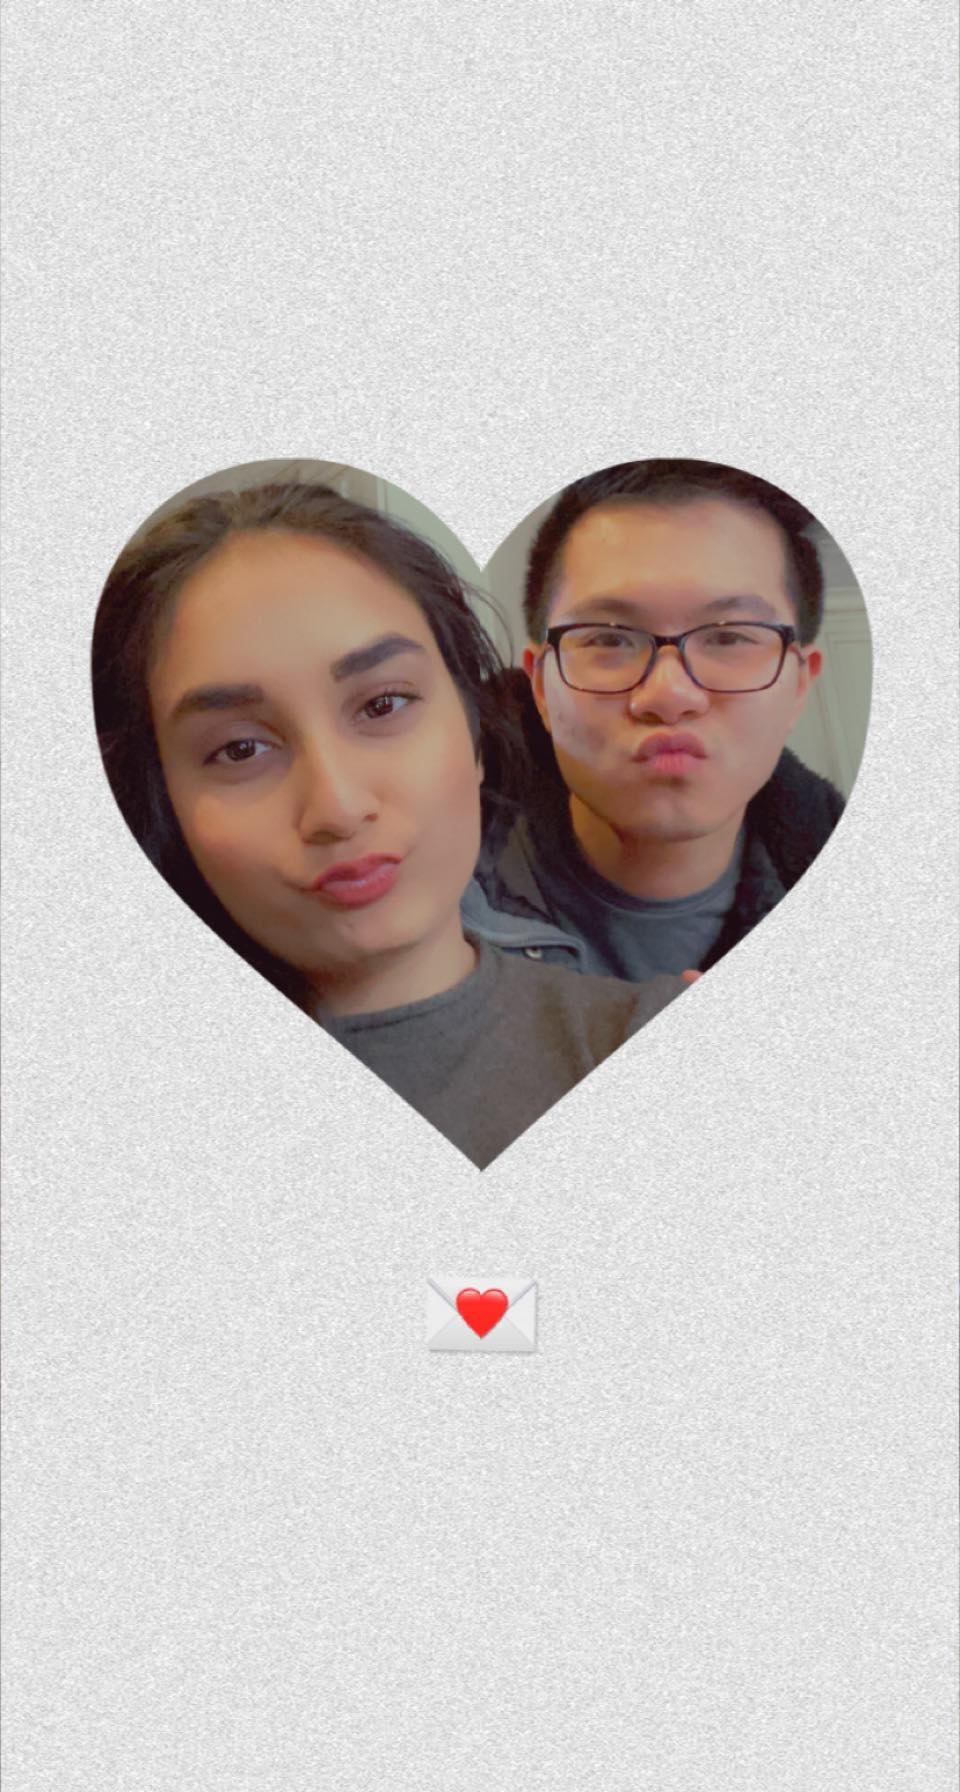
\includegraphics[width=5.20833in,height=\textheight]{mimages/18 3-19-2021.jpg}
\caption{March 19, 2021}
\end{figure}

\hypertarget{preface}{%
\section{Preface}\label{preface}}

\begin{Shaded}
\begin{Highlighting}[]
\NormalTok{The wounds }
\NormalTok{Are reasons }
\NormalTok{I write poetry,}
\NormalTok{To lead us }
\NormalTok{back together.}
\end{Highlighting}
\end{Shaded}

Happy reading!

\hypertarget{to-be-where-you-are}{%
\chapter{To be where you are}\label{to-be-where-you-are}}

\begin{Shaded}
\begin{Highlighting}[]
\NormalTok{I would like to be there,}
\NormalTok{There where ever you are.}
\NormalTok{Pray the weight of the distance is less,}
\NormalTok{Than the weight of luck.}
\NormalTok{The luck of providence to bring us together.}

\NormalTok{The old times,}
\NormalTok{They don}\StringTok{\textquotesingle{}t measure up to the new.}
\StringTok{But the new times,}
\StringTok{They don\textquotesingle{}}\NormalTok{t feel like the old.}
\NormalTok{It}\StringTok{\textquotesingle{}s just how we grow.}

\StringTok{Like that time,}
\StringTok{we went kayaking,}
\StringTok{and within a year }
\StringTok{we came together }
\StringTok{and off we went paddling.}
\end{Highlighting}
\end{Shaded}

\begin{figure}
\centering
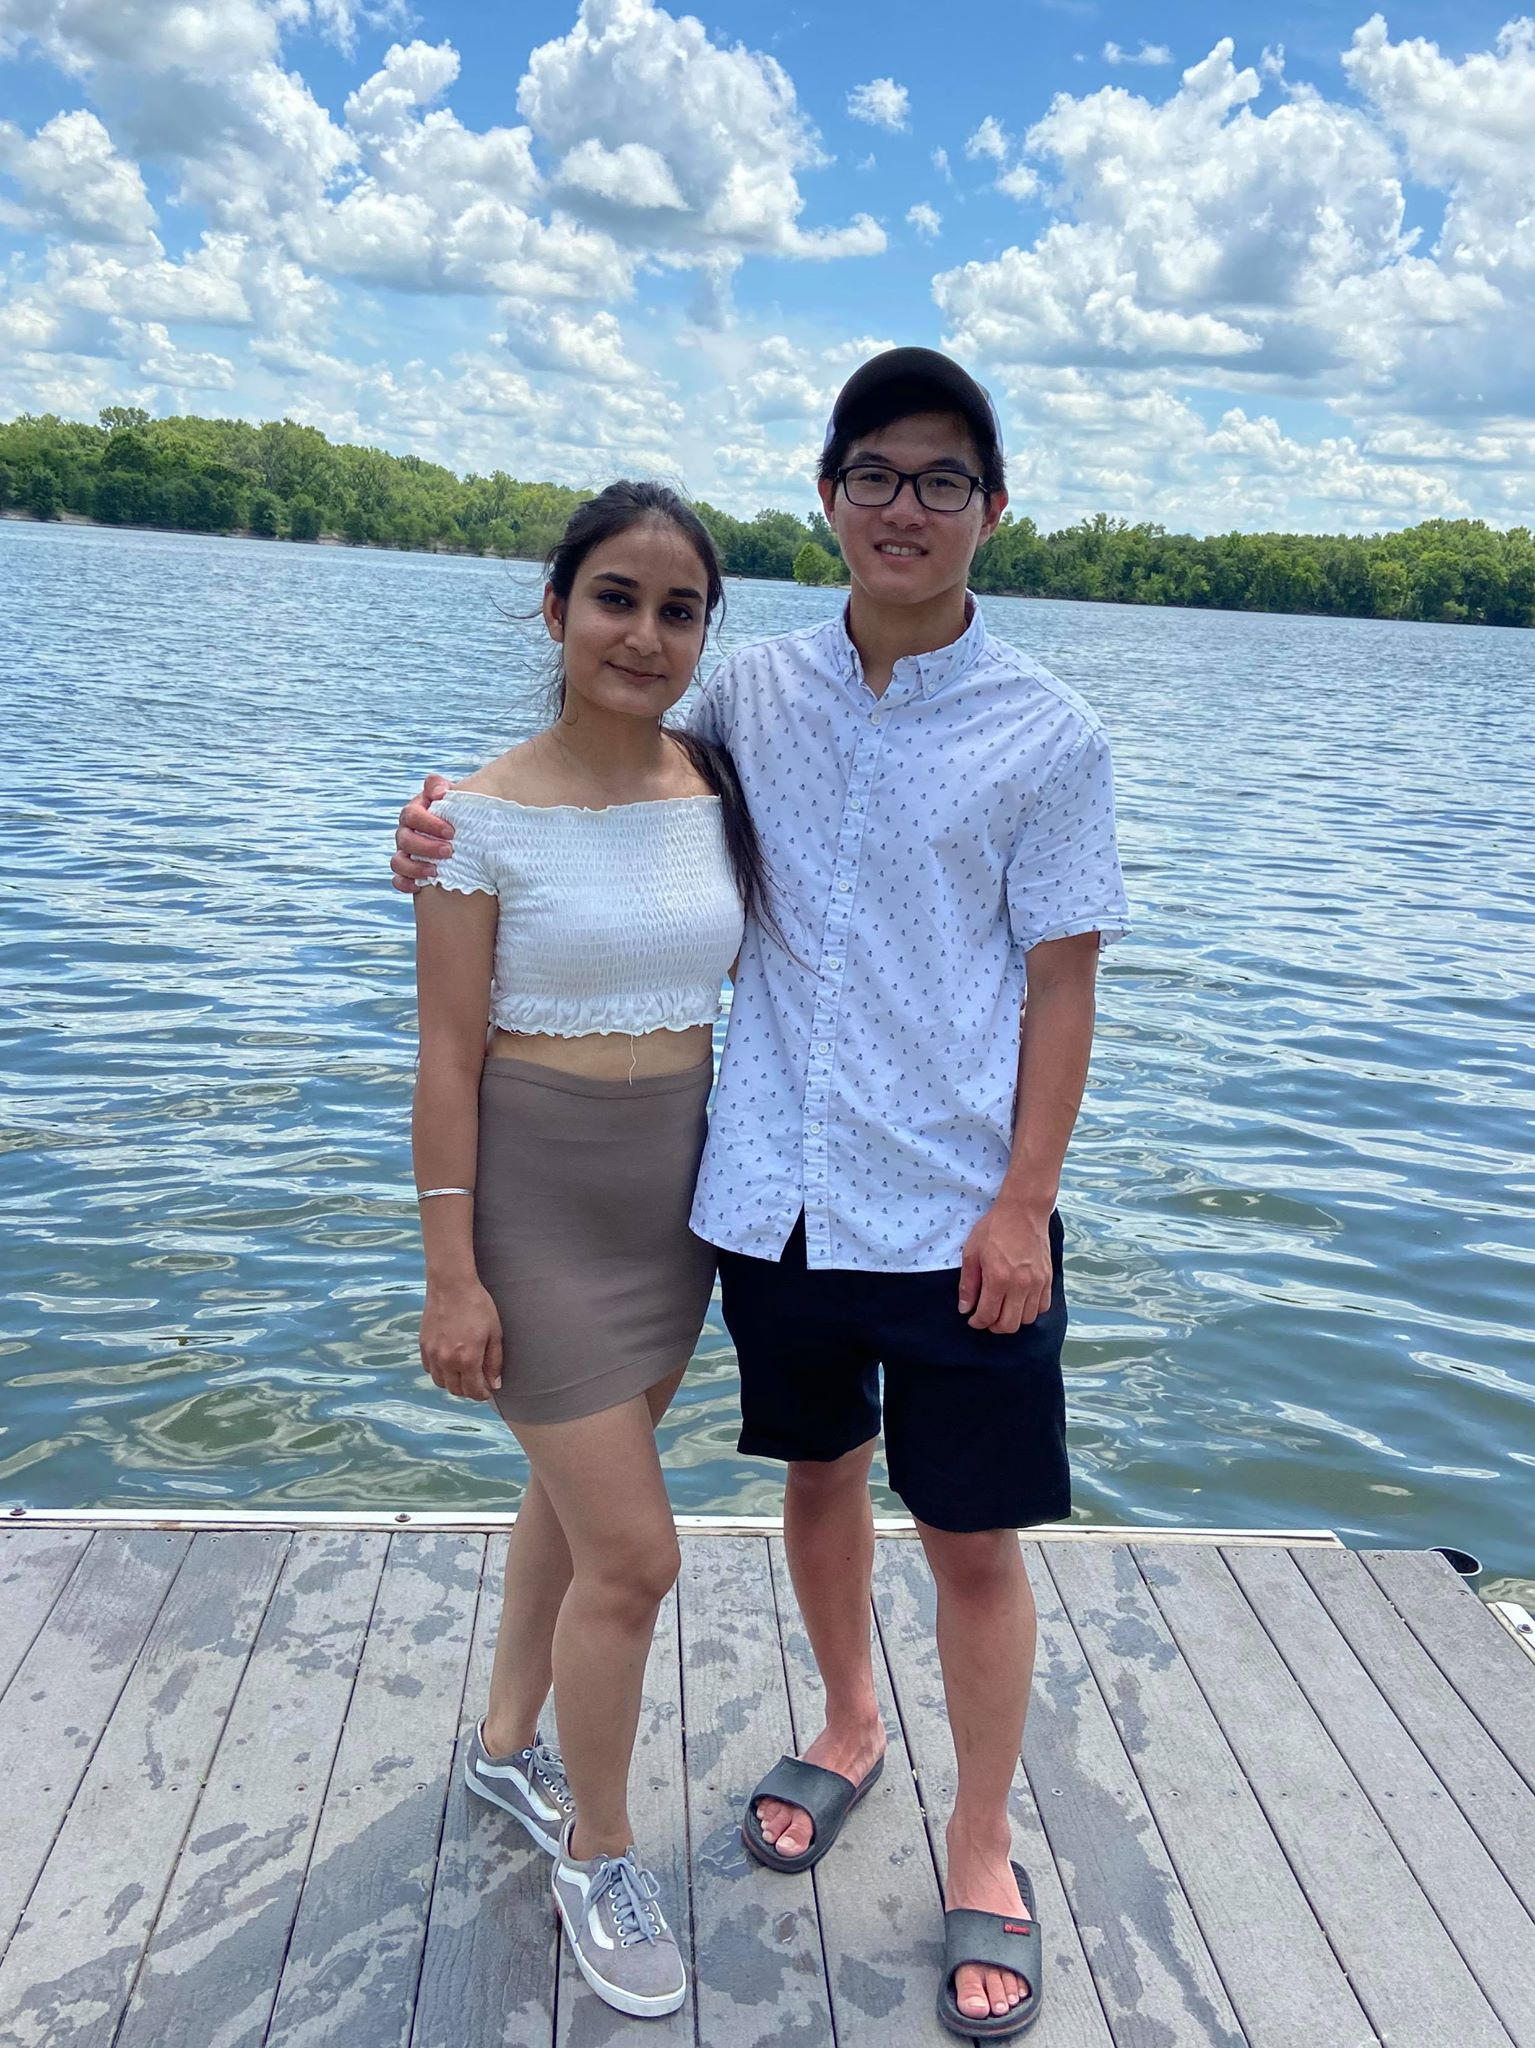
\includegraphics[width=5.20833in,height=\textheight]{images/manjot kayak.jpg}
\caption{July 25, 2020}
\end{figure}

\begin{figure}
\centering
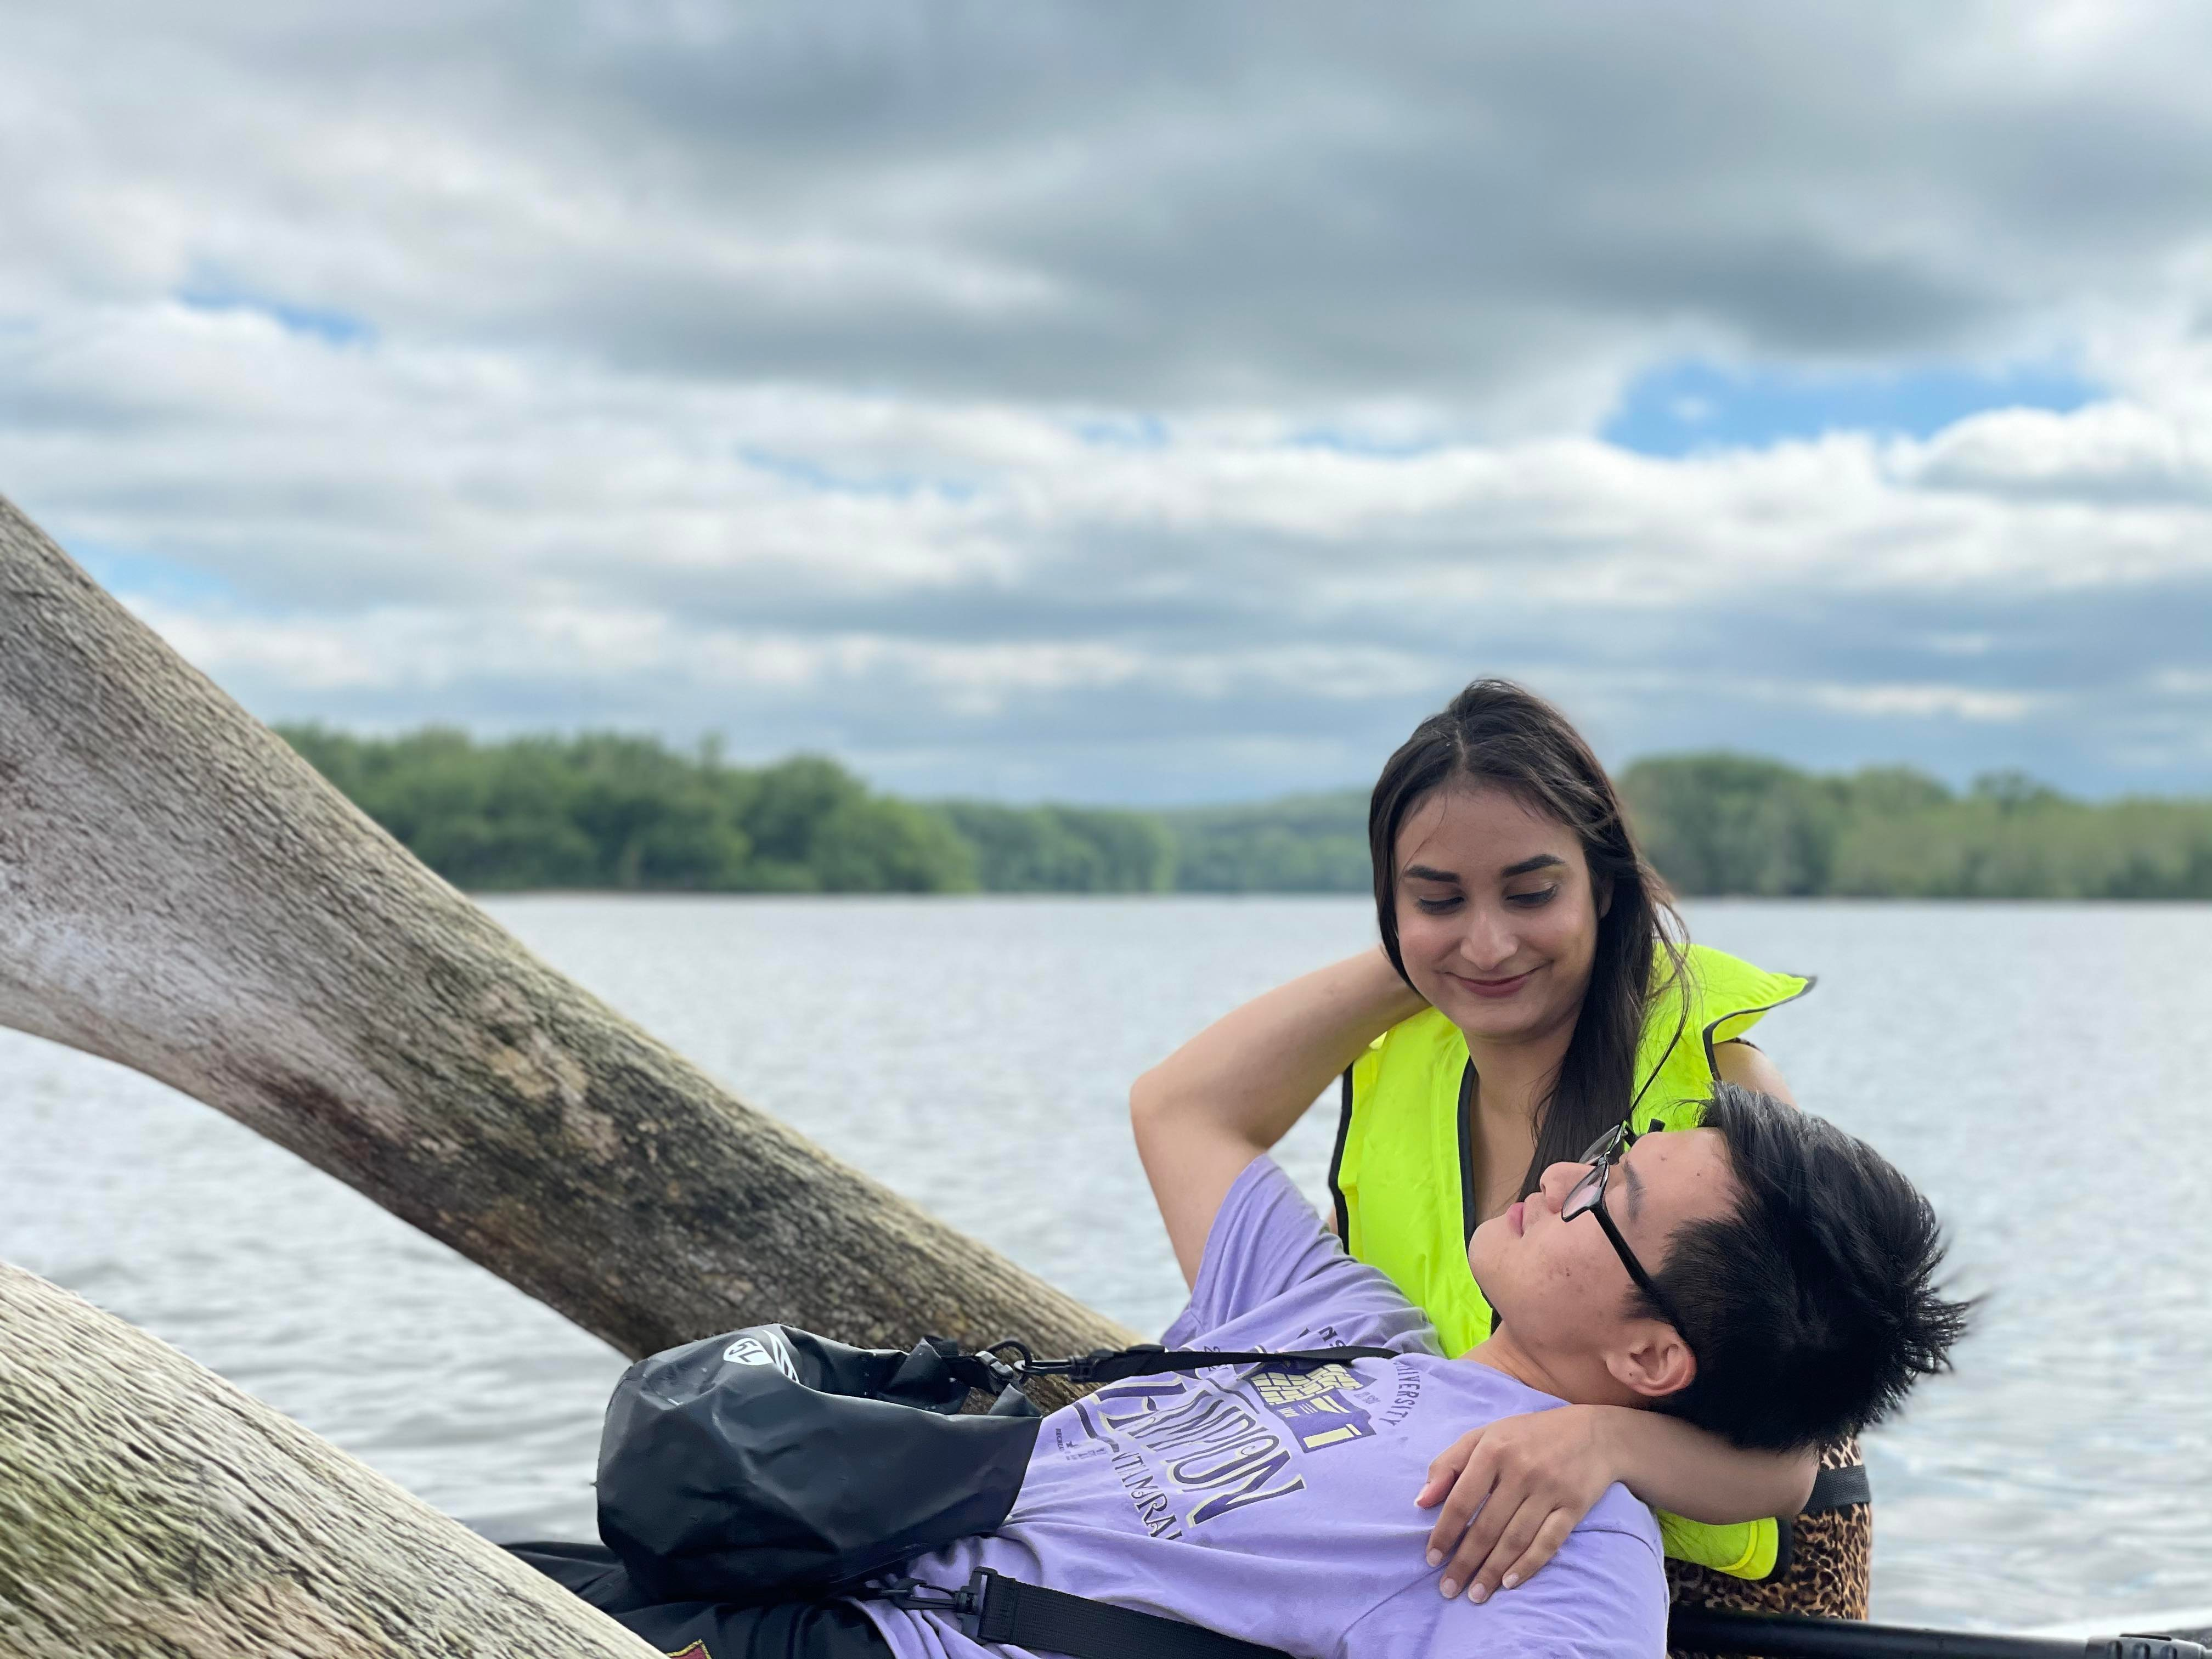
\includegraphics[width=5.20833in,height=\textheight]{mimages/9.1 5-22-2021.jpg}
\caption{May 22, 2021}
\end{figure}

\hypertarget{whatlove-is-or-isnt}{%
\chapter{Whatlove is or isn't}\label{whatlove-is-or-isnt}}

\begin{Shaded}
\begin{Highlighting}[]

\NormalTok{Love isn’t a beautiful spring }\ControlFlowTok{in}\NormalTok{ an enchanted forest,}
\NormalTok{Deep }\ControlFlowTok{in}\NormalTok{ the soft misty dew,}
\NormalTok{Songs from the birds and quaking trees.}

\NormalTok{Love is the ache you feel when she doesn’t pick up the phone,}
\NormalTok{The emptiness you feel waking up,}
\NormalTok{The pain from the distance and different time zones.}

\NormalTok{Love isn’t being comfortable at all times,}
\NormalTok{Having the answers to all of your problems,}
\NormalTok{Giving reasons to stay together forever.}

\NormalTok{Love is sharing our scars,}
\NormalTok{Counting the days till we see each other,}
\NormalTok{Waking up late and starting the day beyond normal.}

\NormalTok{Love isn’t rational like math and science,}
\NormalTok{It is responsible }\ControlFlowTok{for}\NormalTok{ being irresponsible, }
\NormalTok{It is the feeling of fullness and belonging.}

\NormalTok{Even when my hair is bushy and my clothes are baggy,}
\NormalTok{When my English isn}\StringTok{\textquotesingle{}t English,}
\StringTok{When my body isn\textquotesingle{}}\NormalTok{t as distinguished,}

\NormalTok{You accept me }\ControlFlowTok{for}\NormalTok{ me,}
\NormalTok{And I accept you }\ControlFlowTok{for}\NormalTok{ you.}
\end{Highlighting}
\end{Shaded}

\begin{figure}
\centering
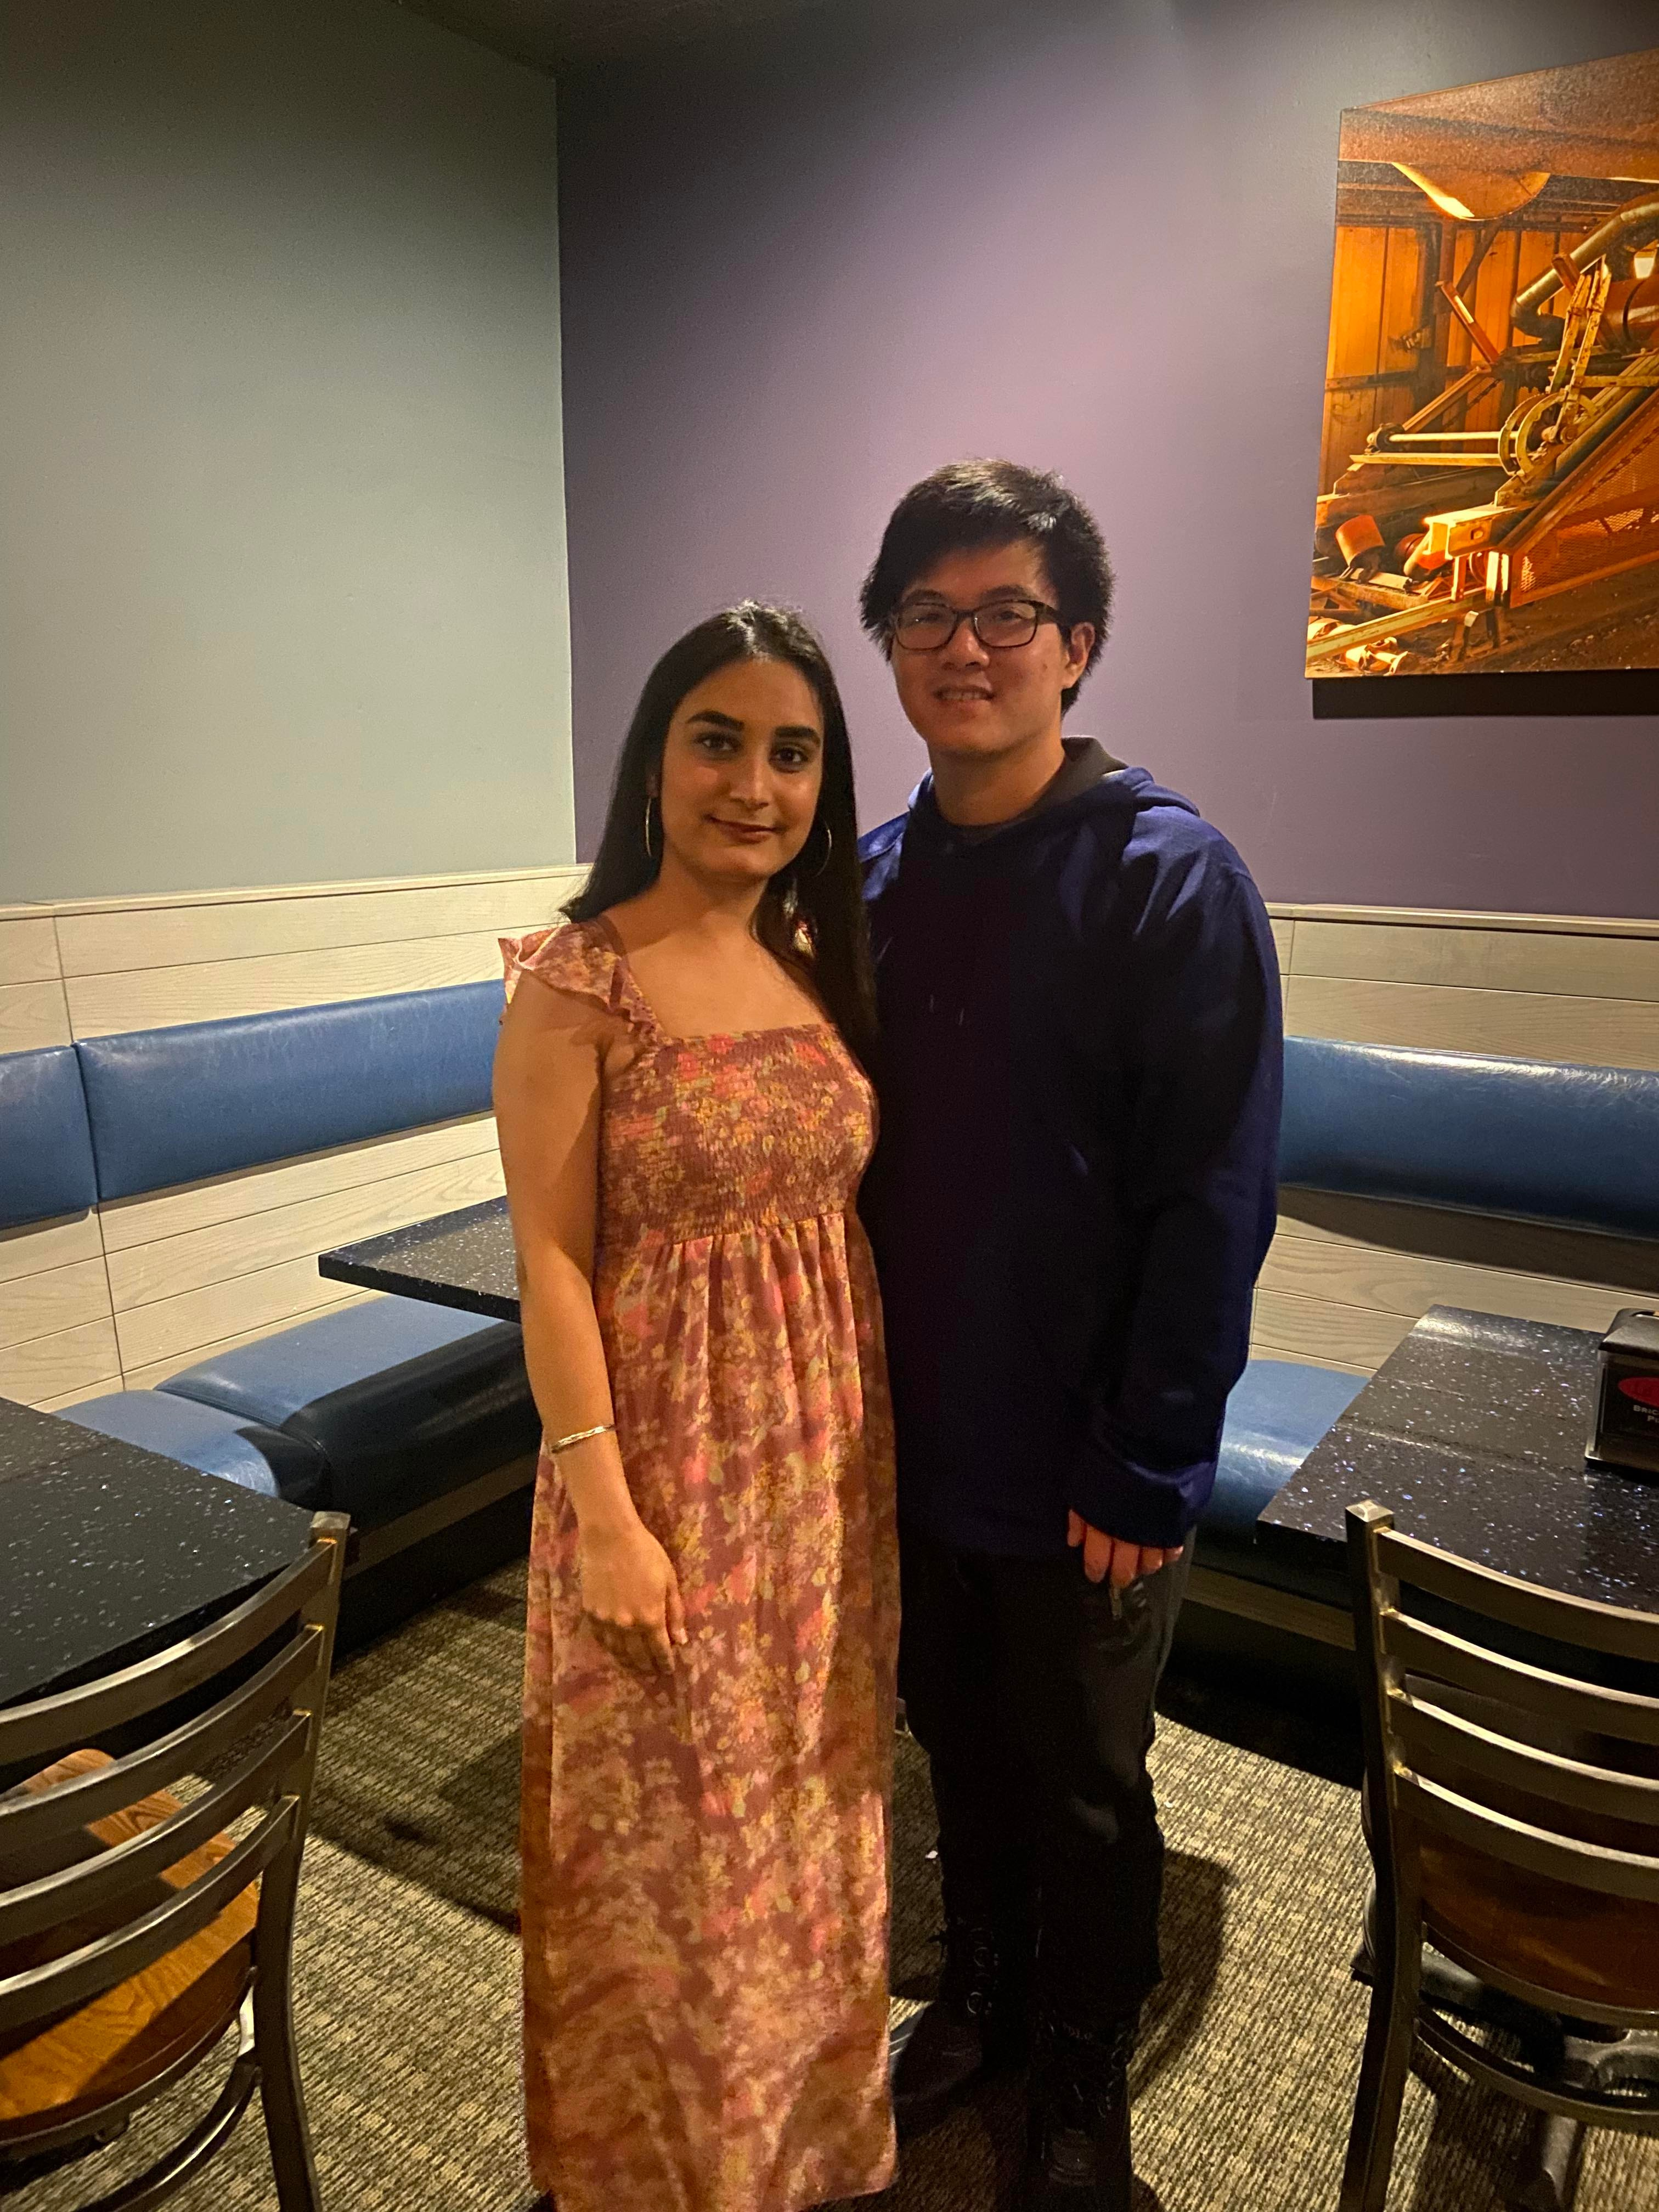
\includegraphics[width=5.20833in,height=\textheight]{mimages/16 2-16-2021.jpg}
\caption{February 15, 2021}
\end{figure}

\begin{figure}
\centering
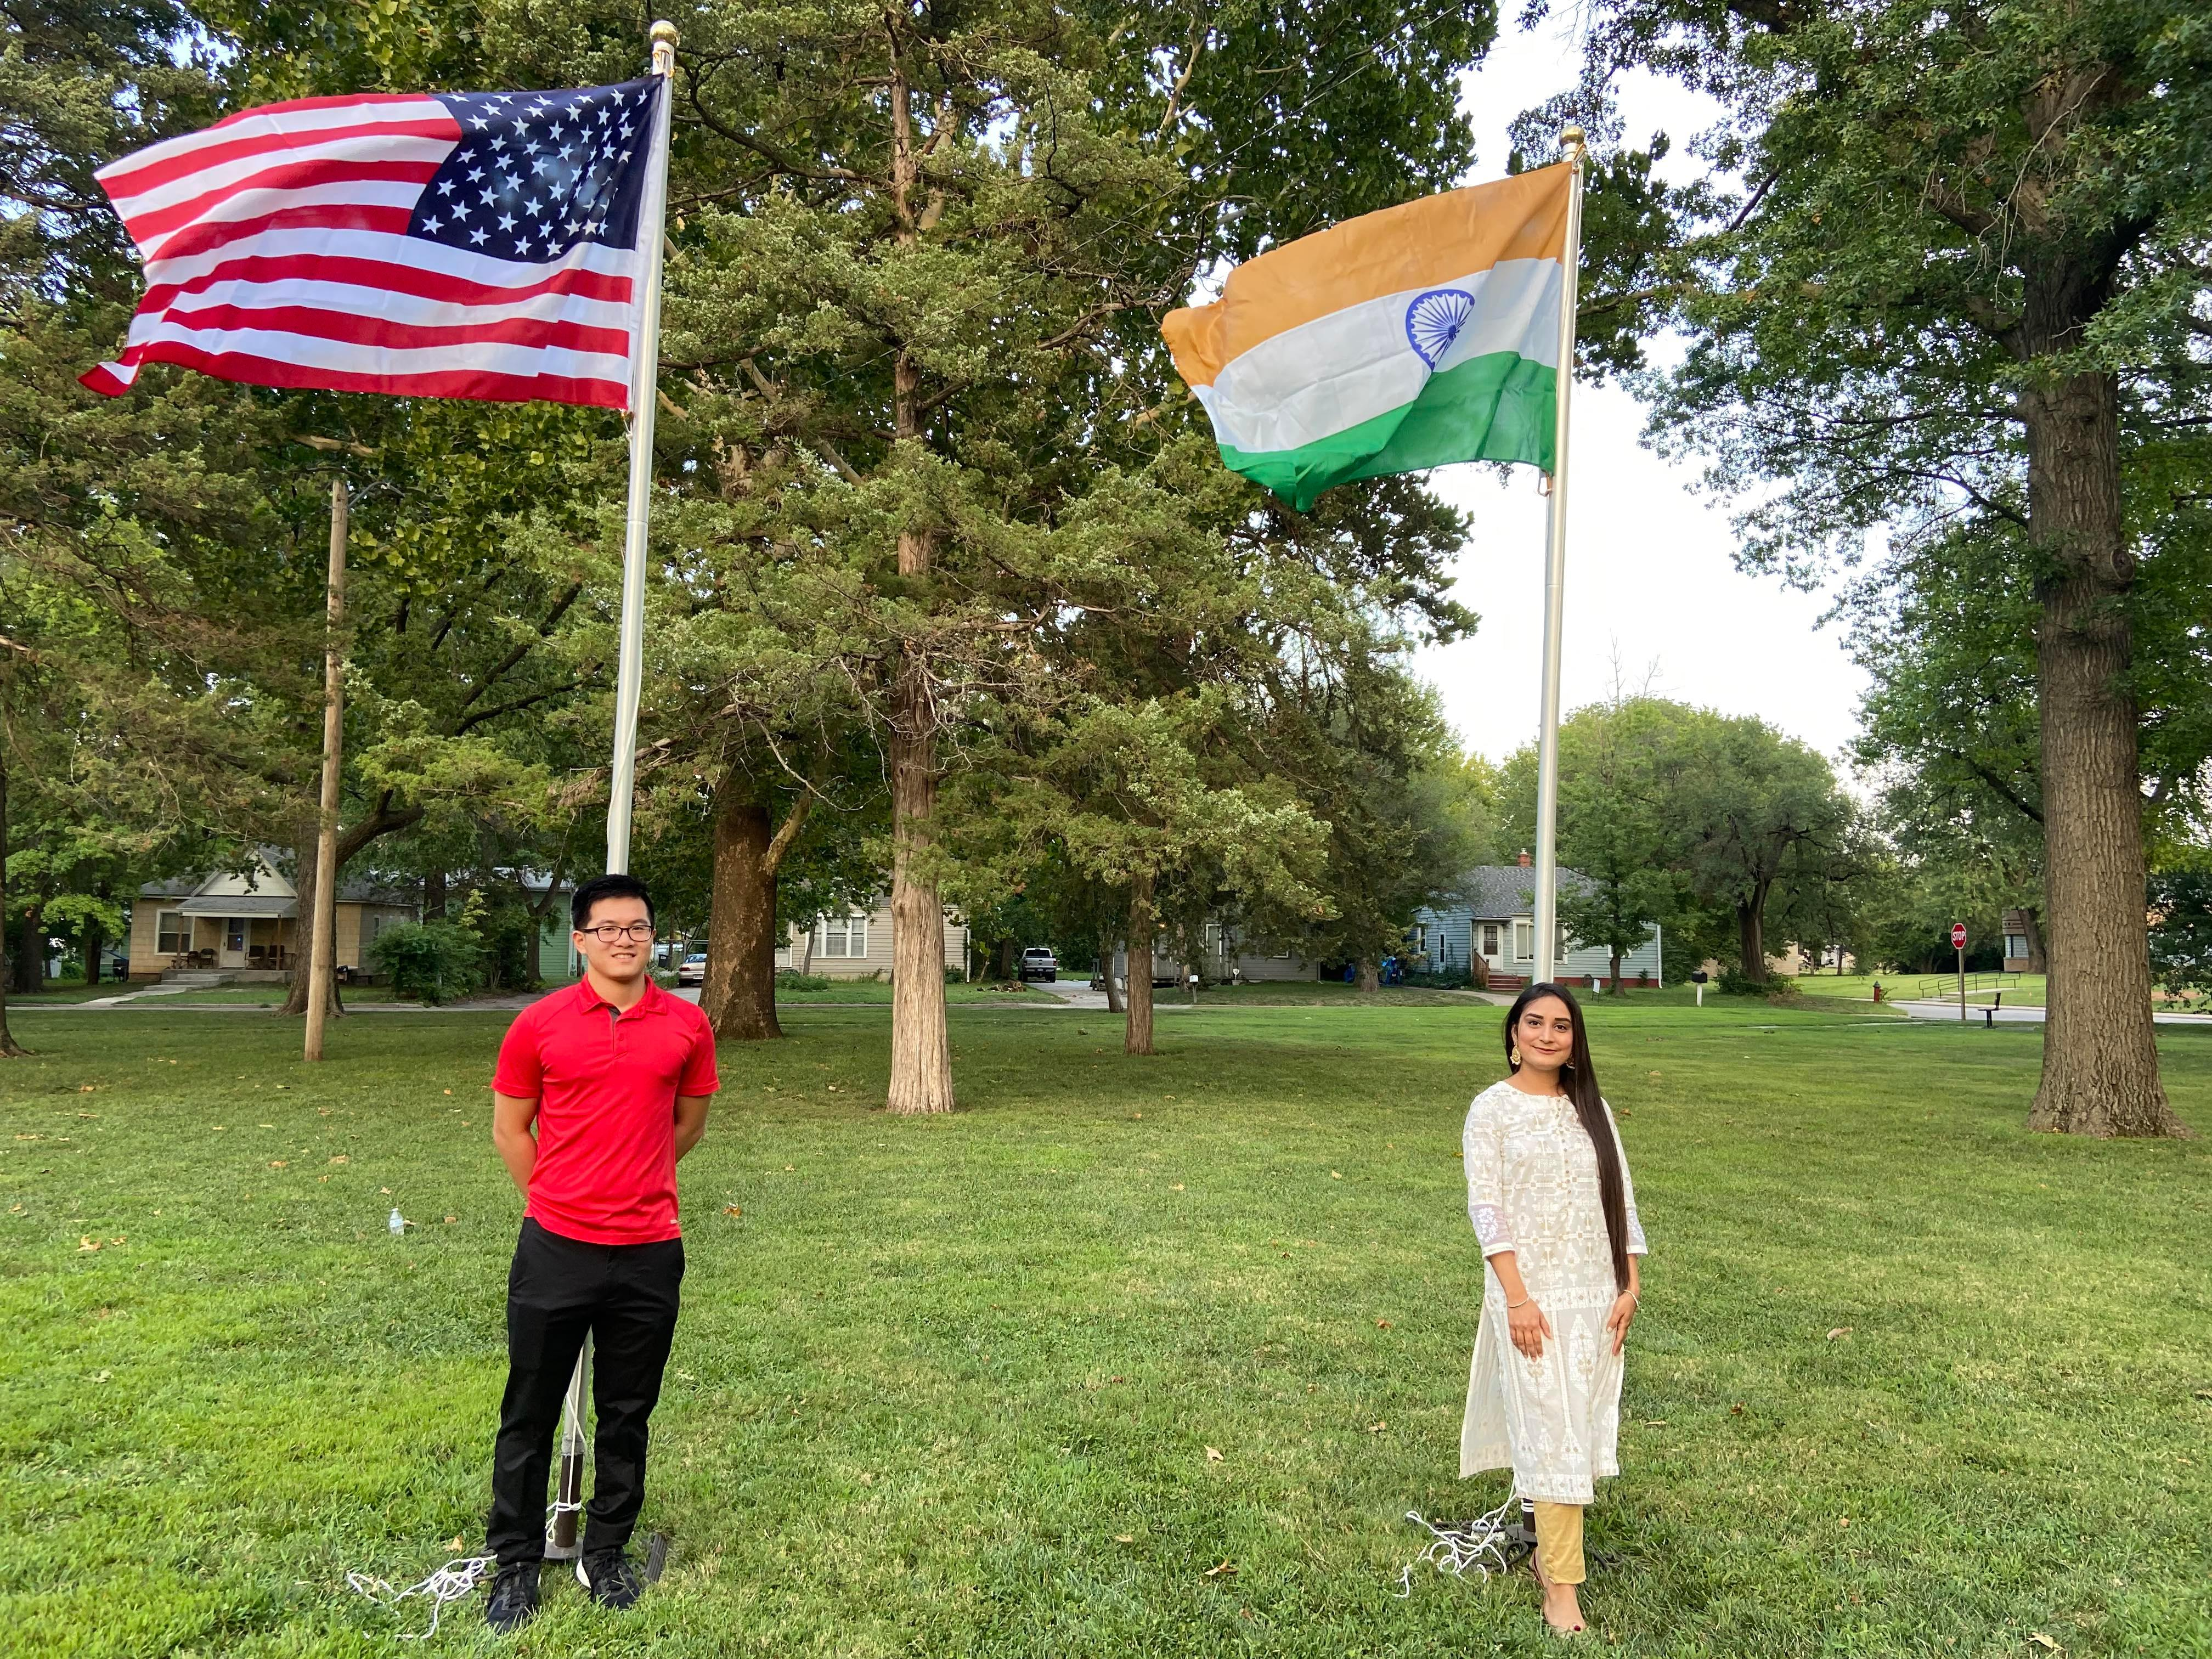
\includegraphics[width=5.20833in,height=\textheight]{mimages/12.1 8-15-2021.jpg}
\caption{August 15, 2021}
\end{figure}

\begin{figure}
\centering
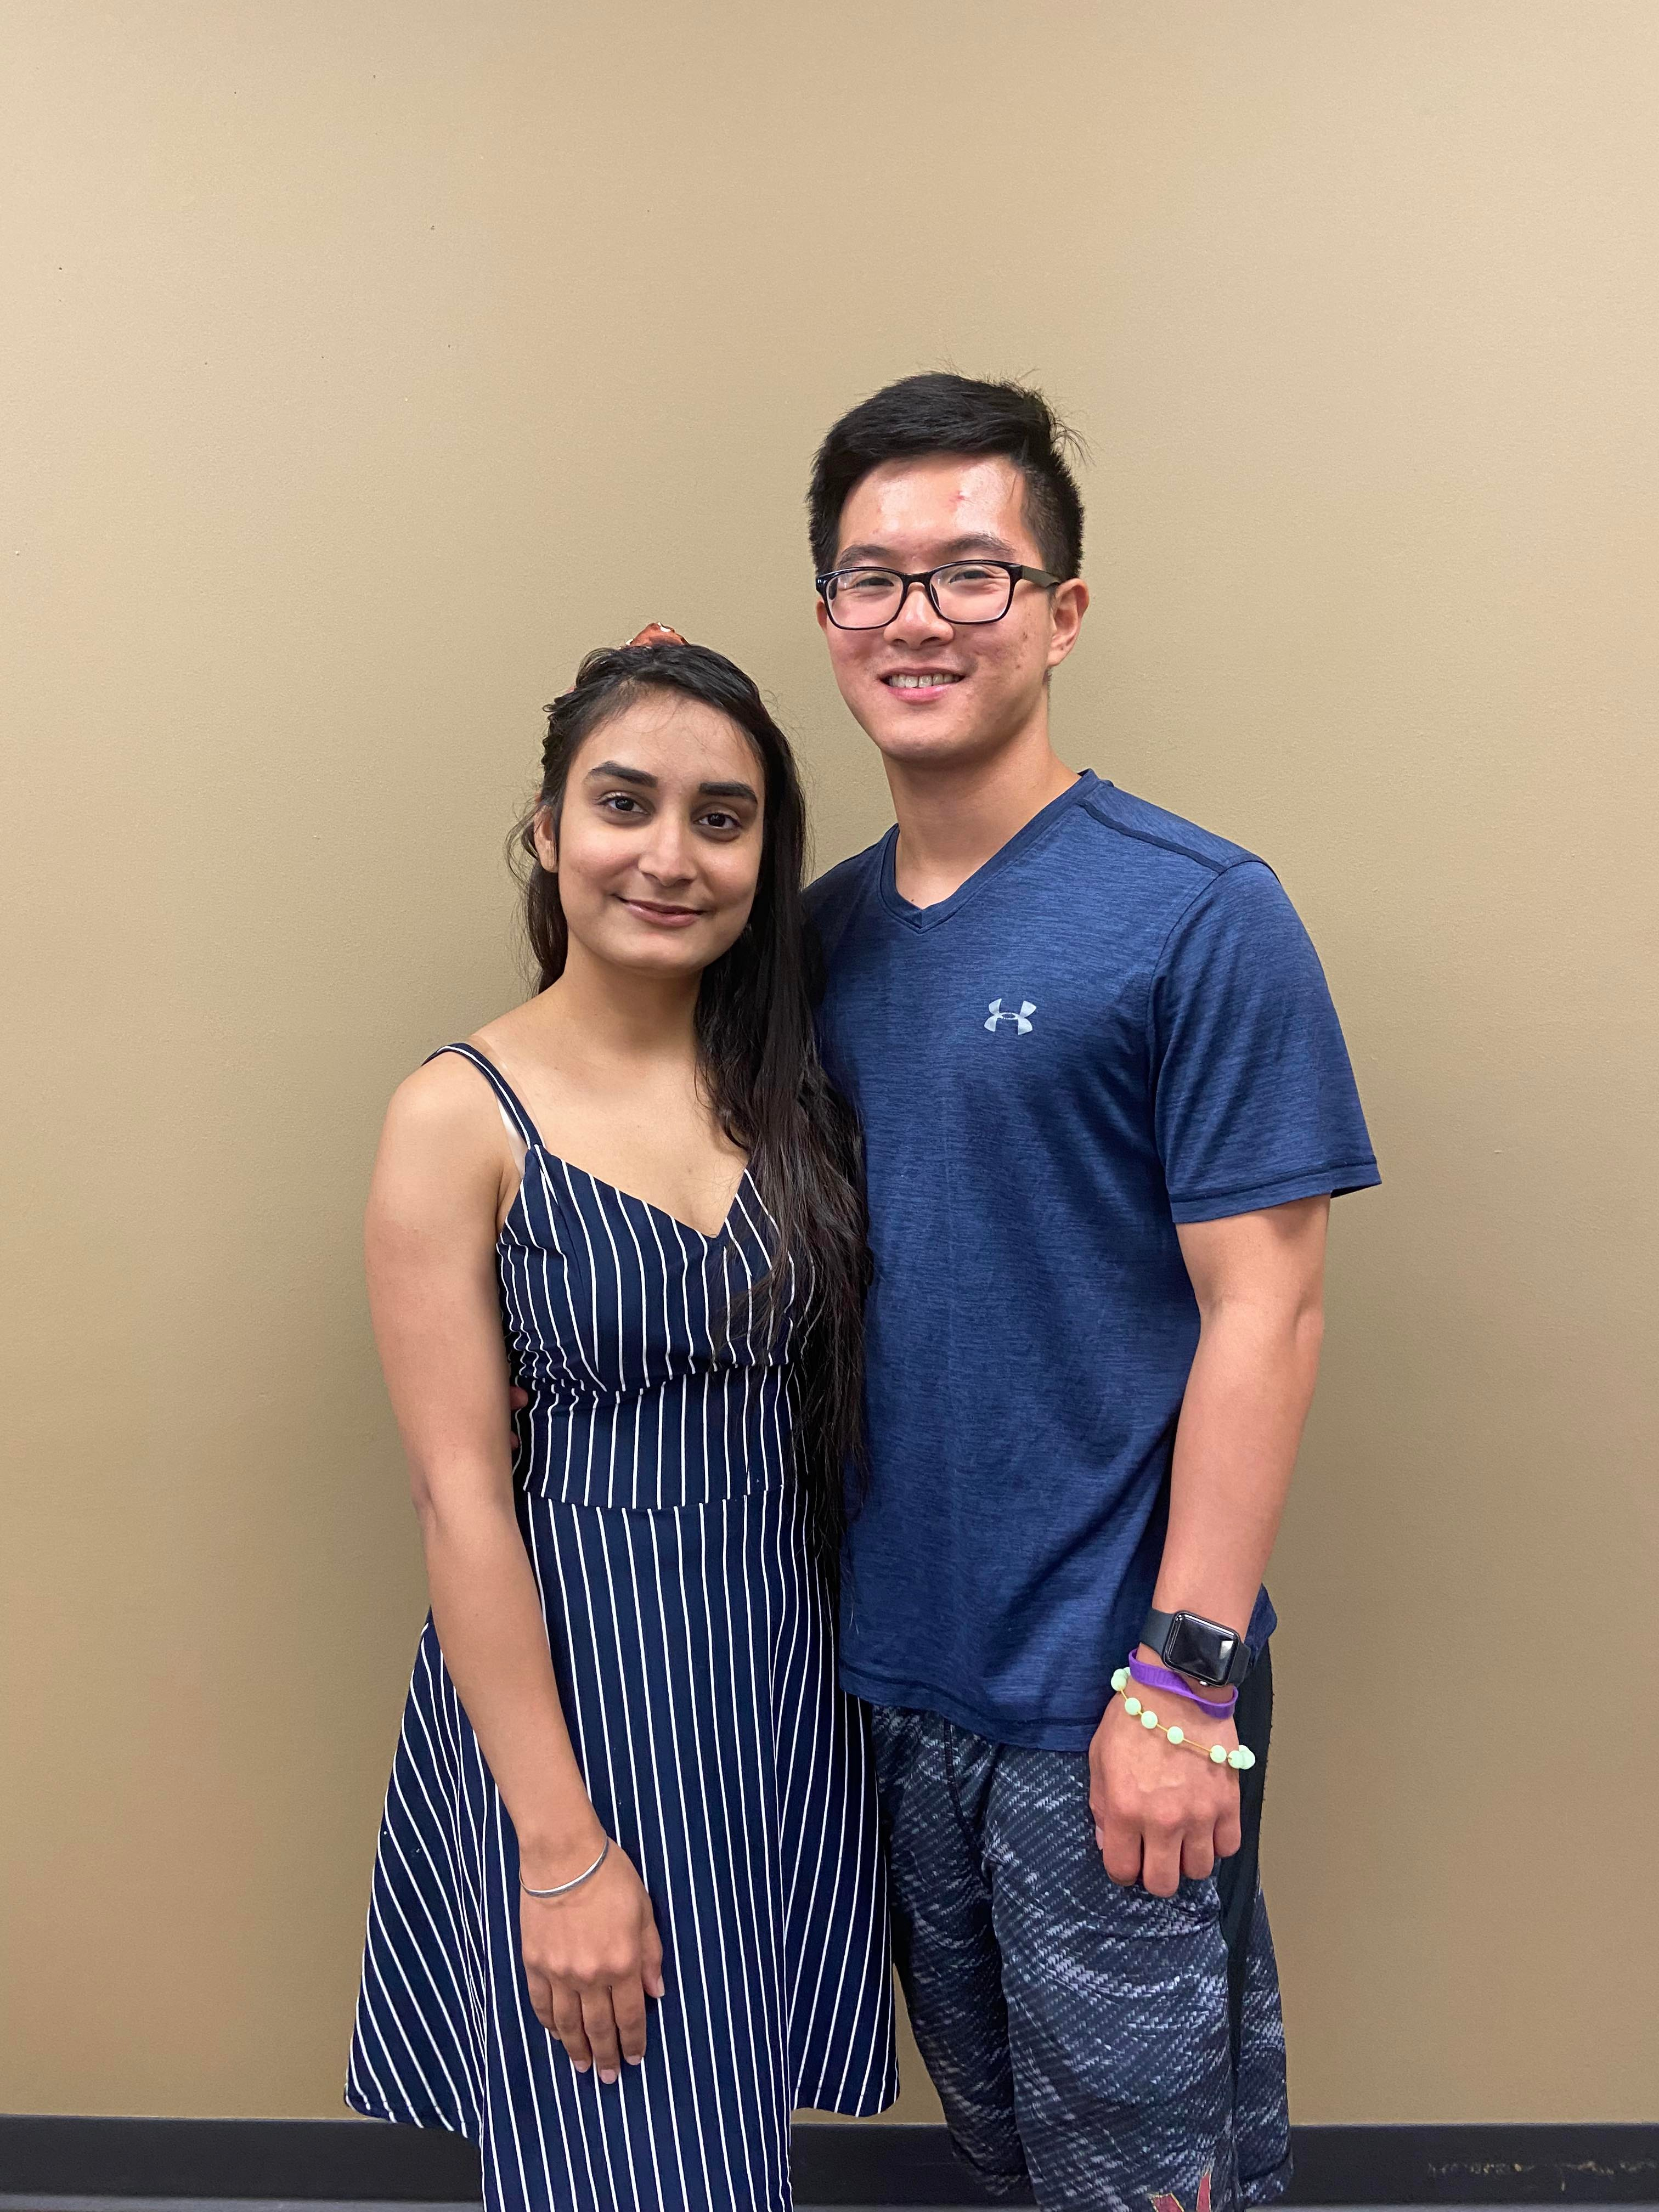
\includegraphics[width=5.20833in,height=\textheight]{mimages/11.1 7-3-2021.jpg}
\caption{July 3, 2021}
\end{figure}

\hypertarget{family}{%
\chapter{Family}\label{family}}

\begin{Shaded}
\begin{Highlighting}[]
\NormalTok{When I was a kid,}
\NormalTok{I went to temple on Saturdays,}
\NormalTok{and church on Sundays,}
\NormalTok{To hear the preacher preach.}

\NormalTok{We sang, ate, and played.}
\NormalTok{They made me think about my life,}
\NormalTok{The good, the bad,}
\NormalTok{and everything }\ControlFlowTok{in}\NormalTok{ between.}

\NormalTok{Those days cannot be}
\NormalTok{these days.}
\NormalTok{But I can make these days}
\NormalTok{better days.}

\NormalTok{With someone,}
\NormalTok{Someone,}
\NormalTok{specifically,}
\NormalTok{YOU}\SpecialCharTok{!}
\end{Highlighting}
\end{Shaded}

\begin{figure}
\centering
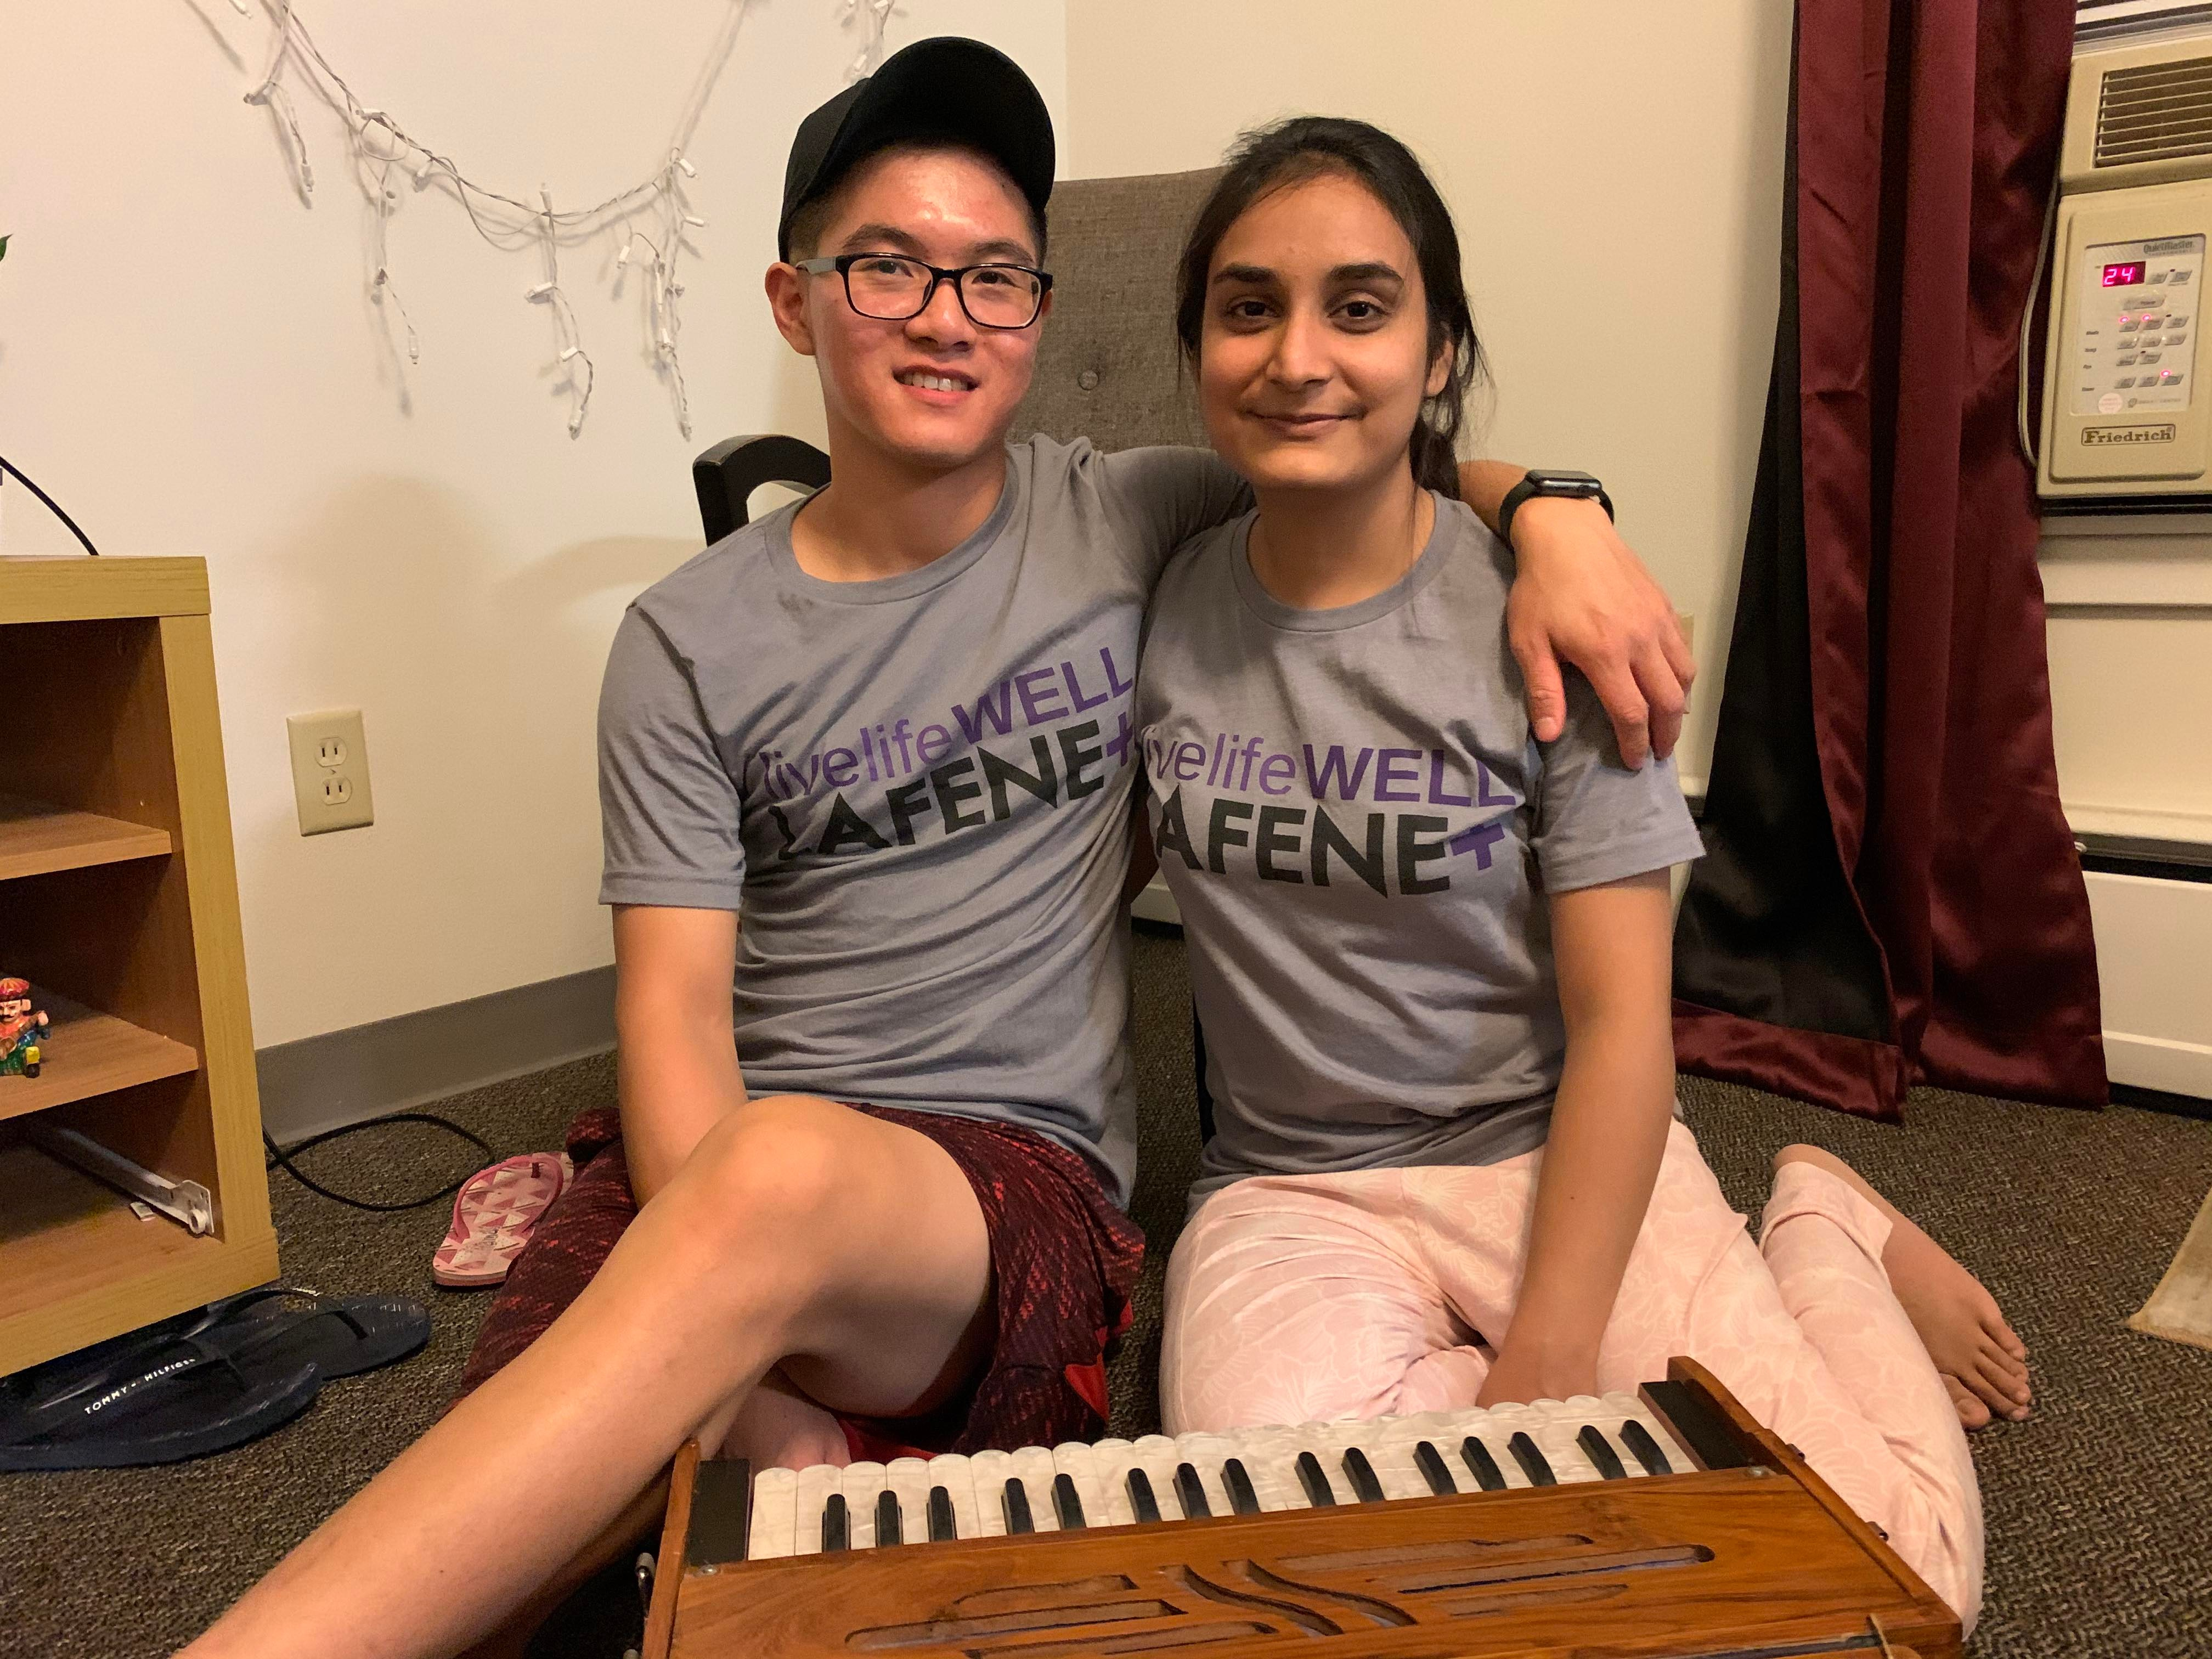
\includegraphics[width=5.20833in,height=\textheight]{mimages/1 9-2-2020.jpg}
\caption{September 2, 2020}
\end{figure}

\begin{figure}
\centering
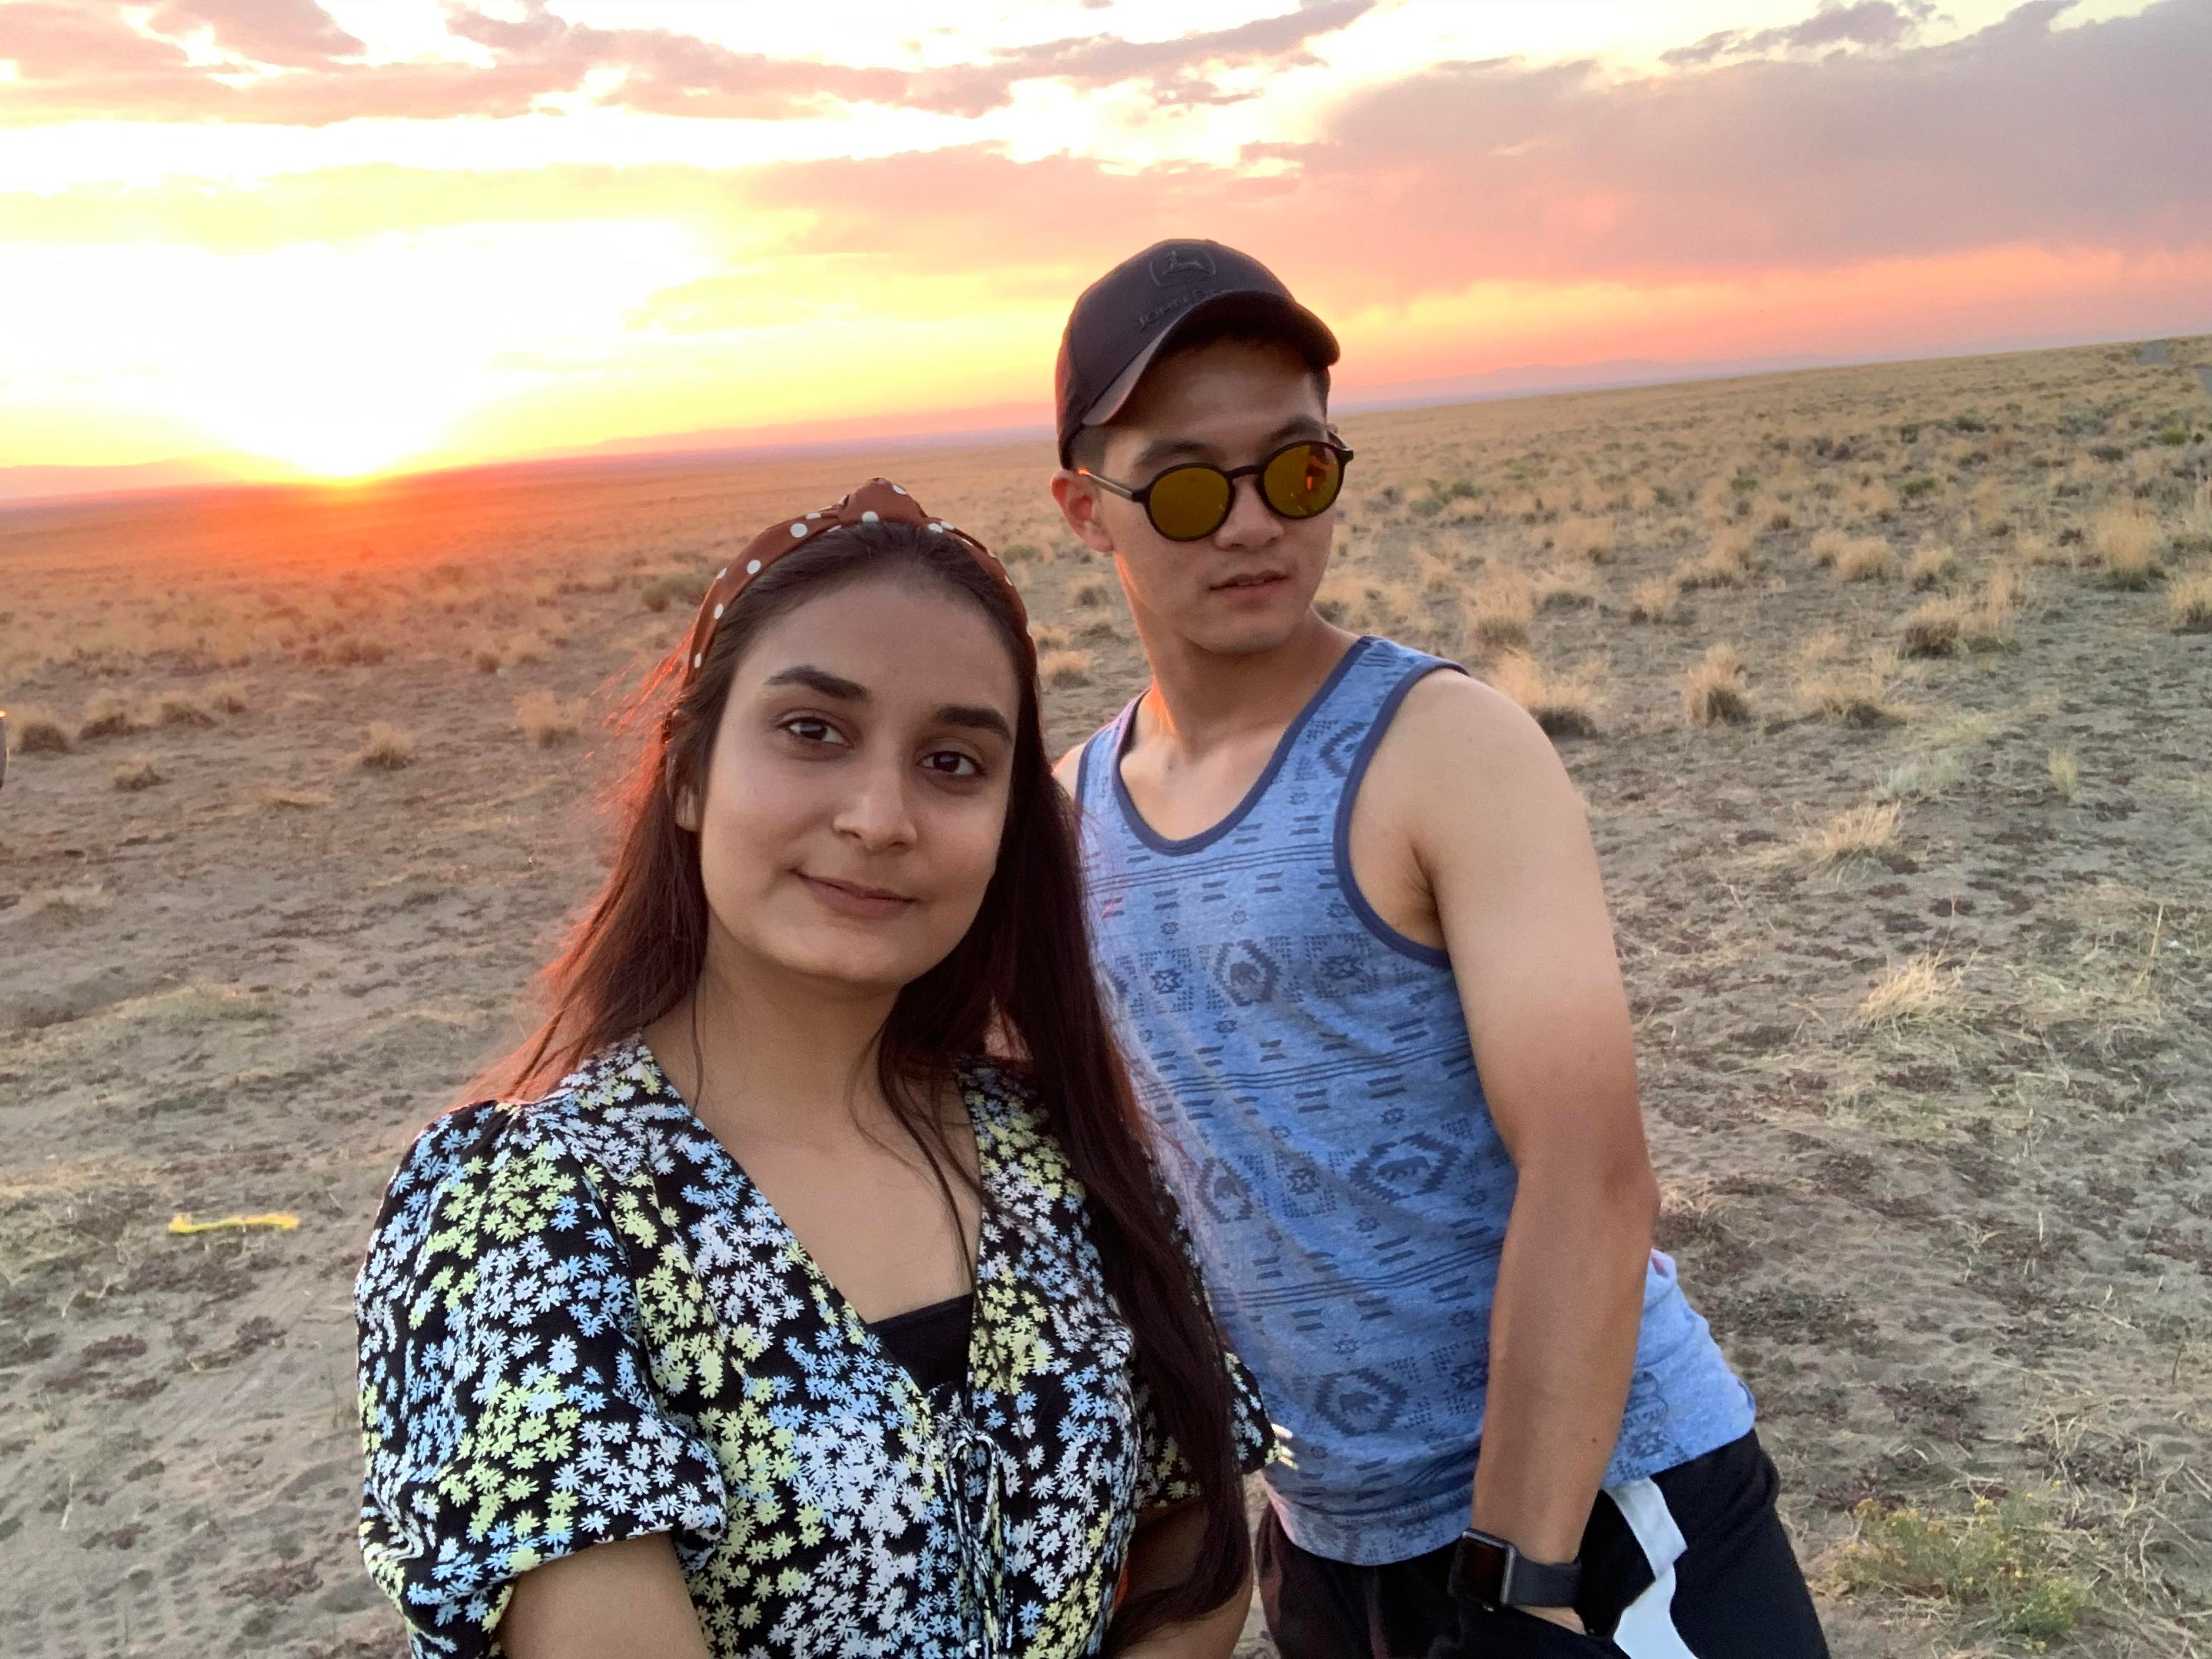
\includegraphics[width=5.20833in,height=\textheight]{mimages/2 9-6-2020.jpg}
\caption{September 6, 2020}
\end{figure}

\begin{figure}
\centering
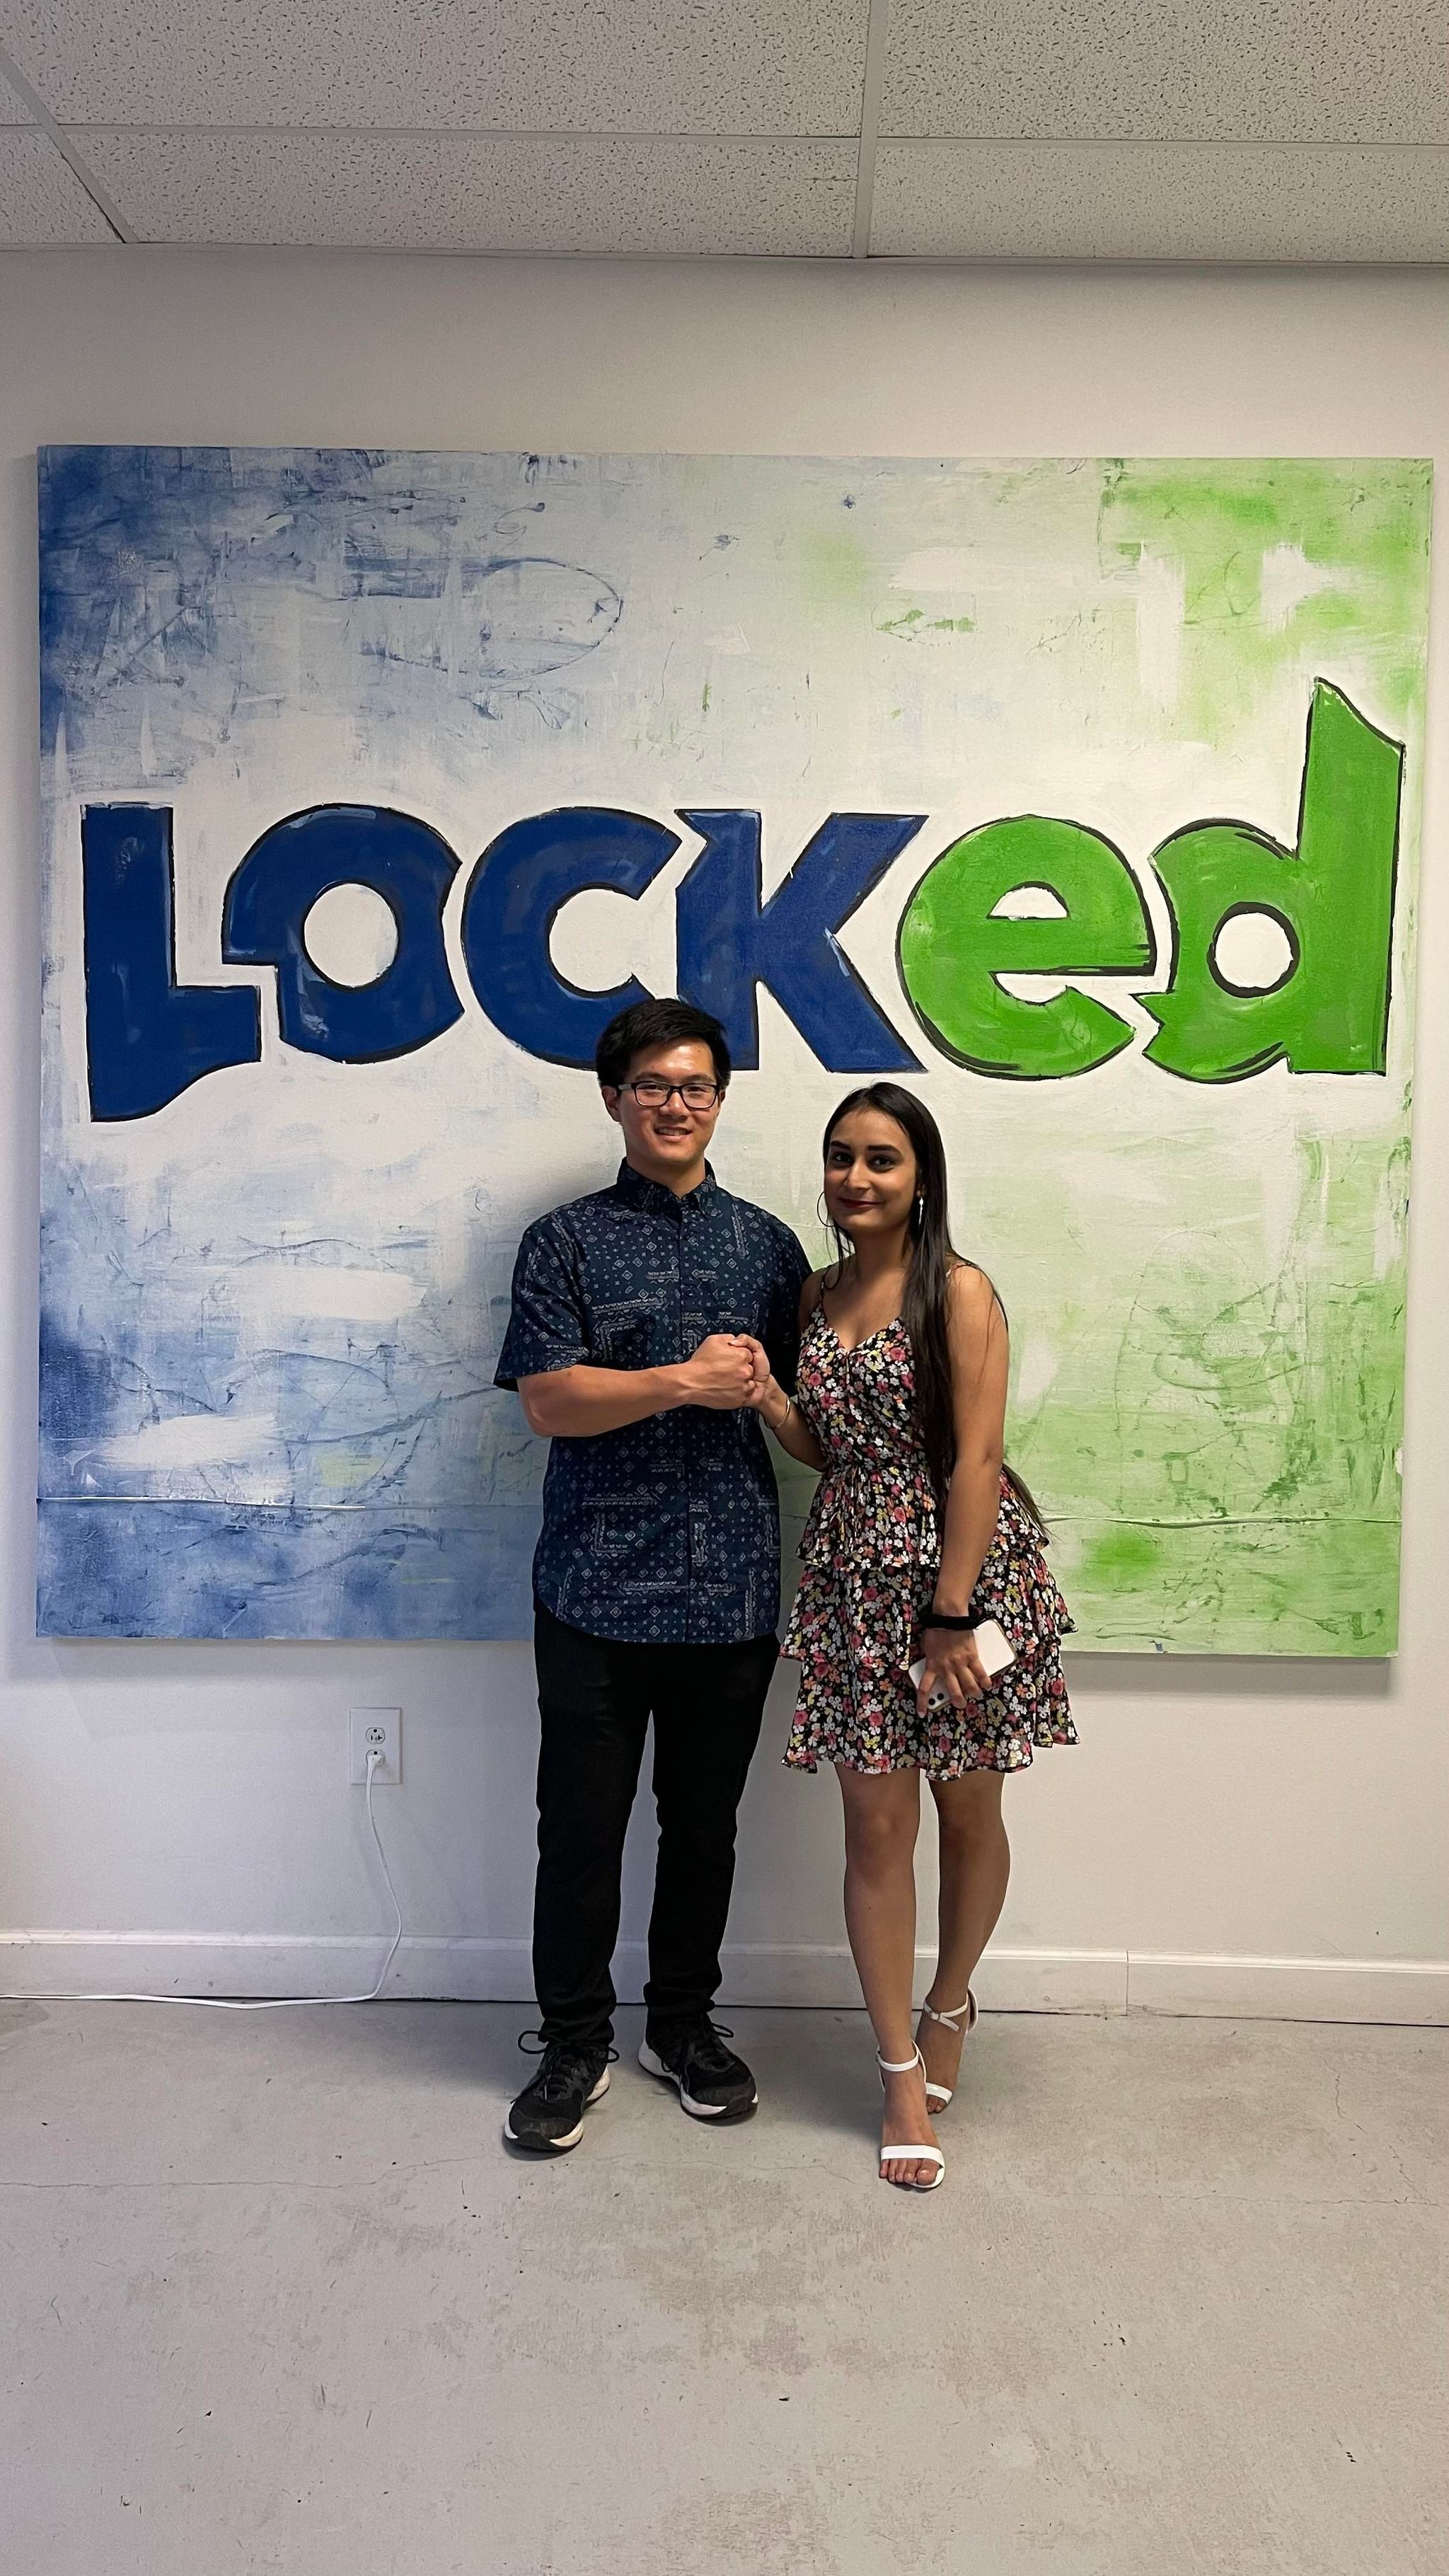
\includegraphics[width=5.20833in,height=\textheight]{mimages/13 9-11-2021.jpg}
\caption{September 11, 2021}
\end{figure}

\begin{figure}
\centering
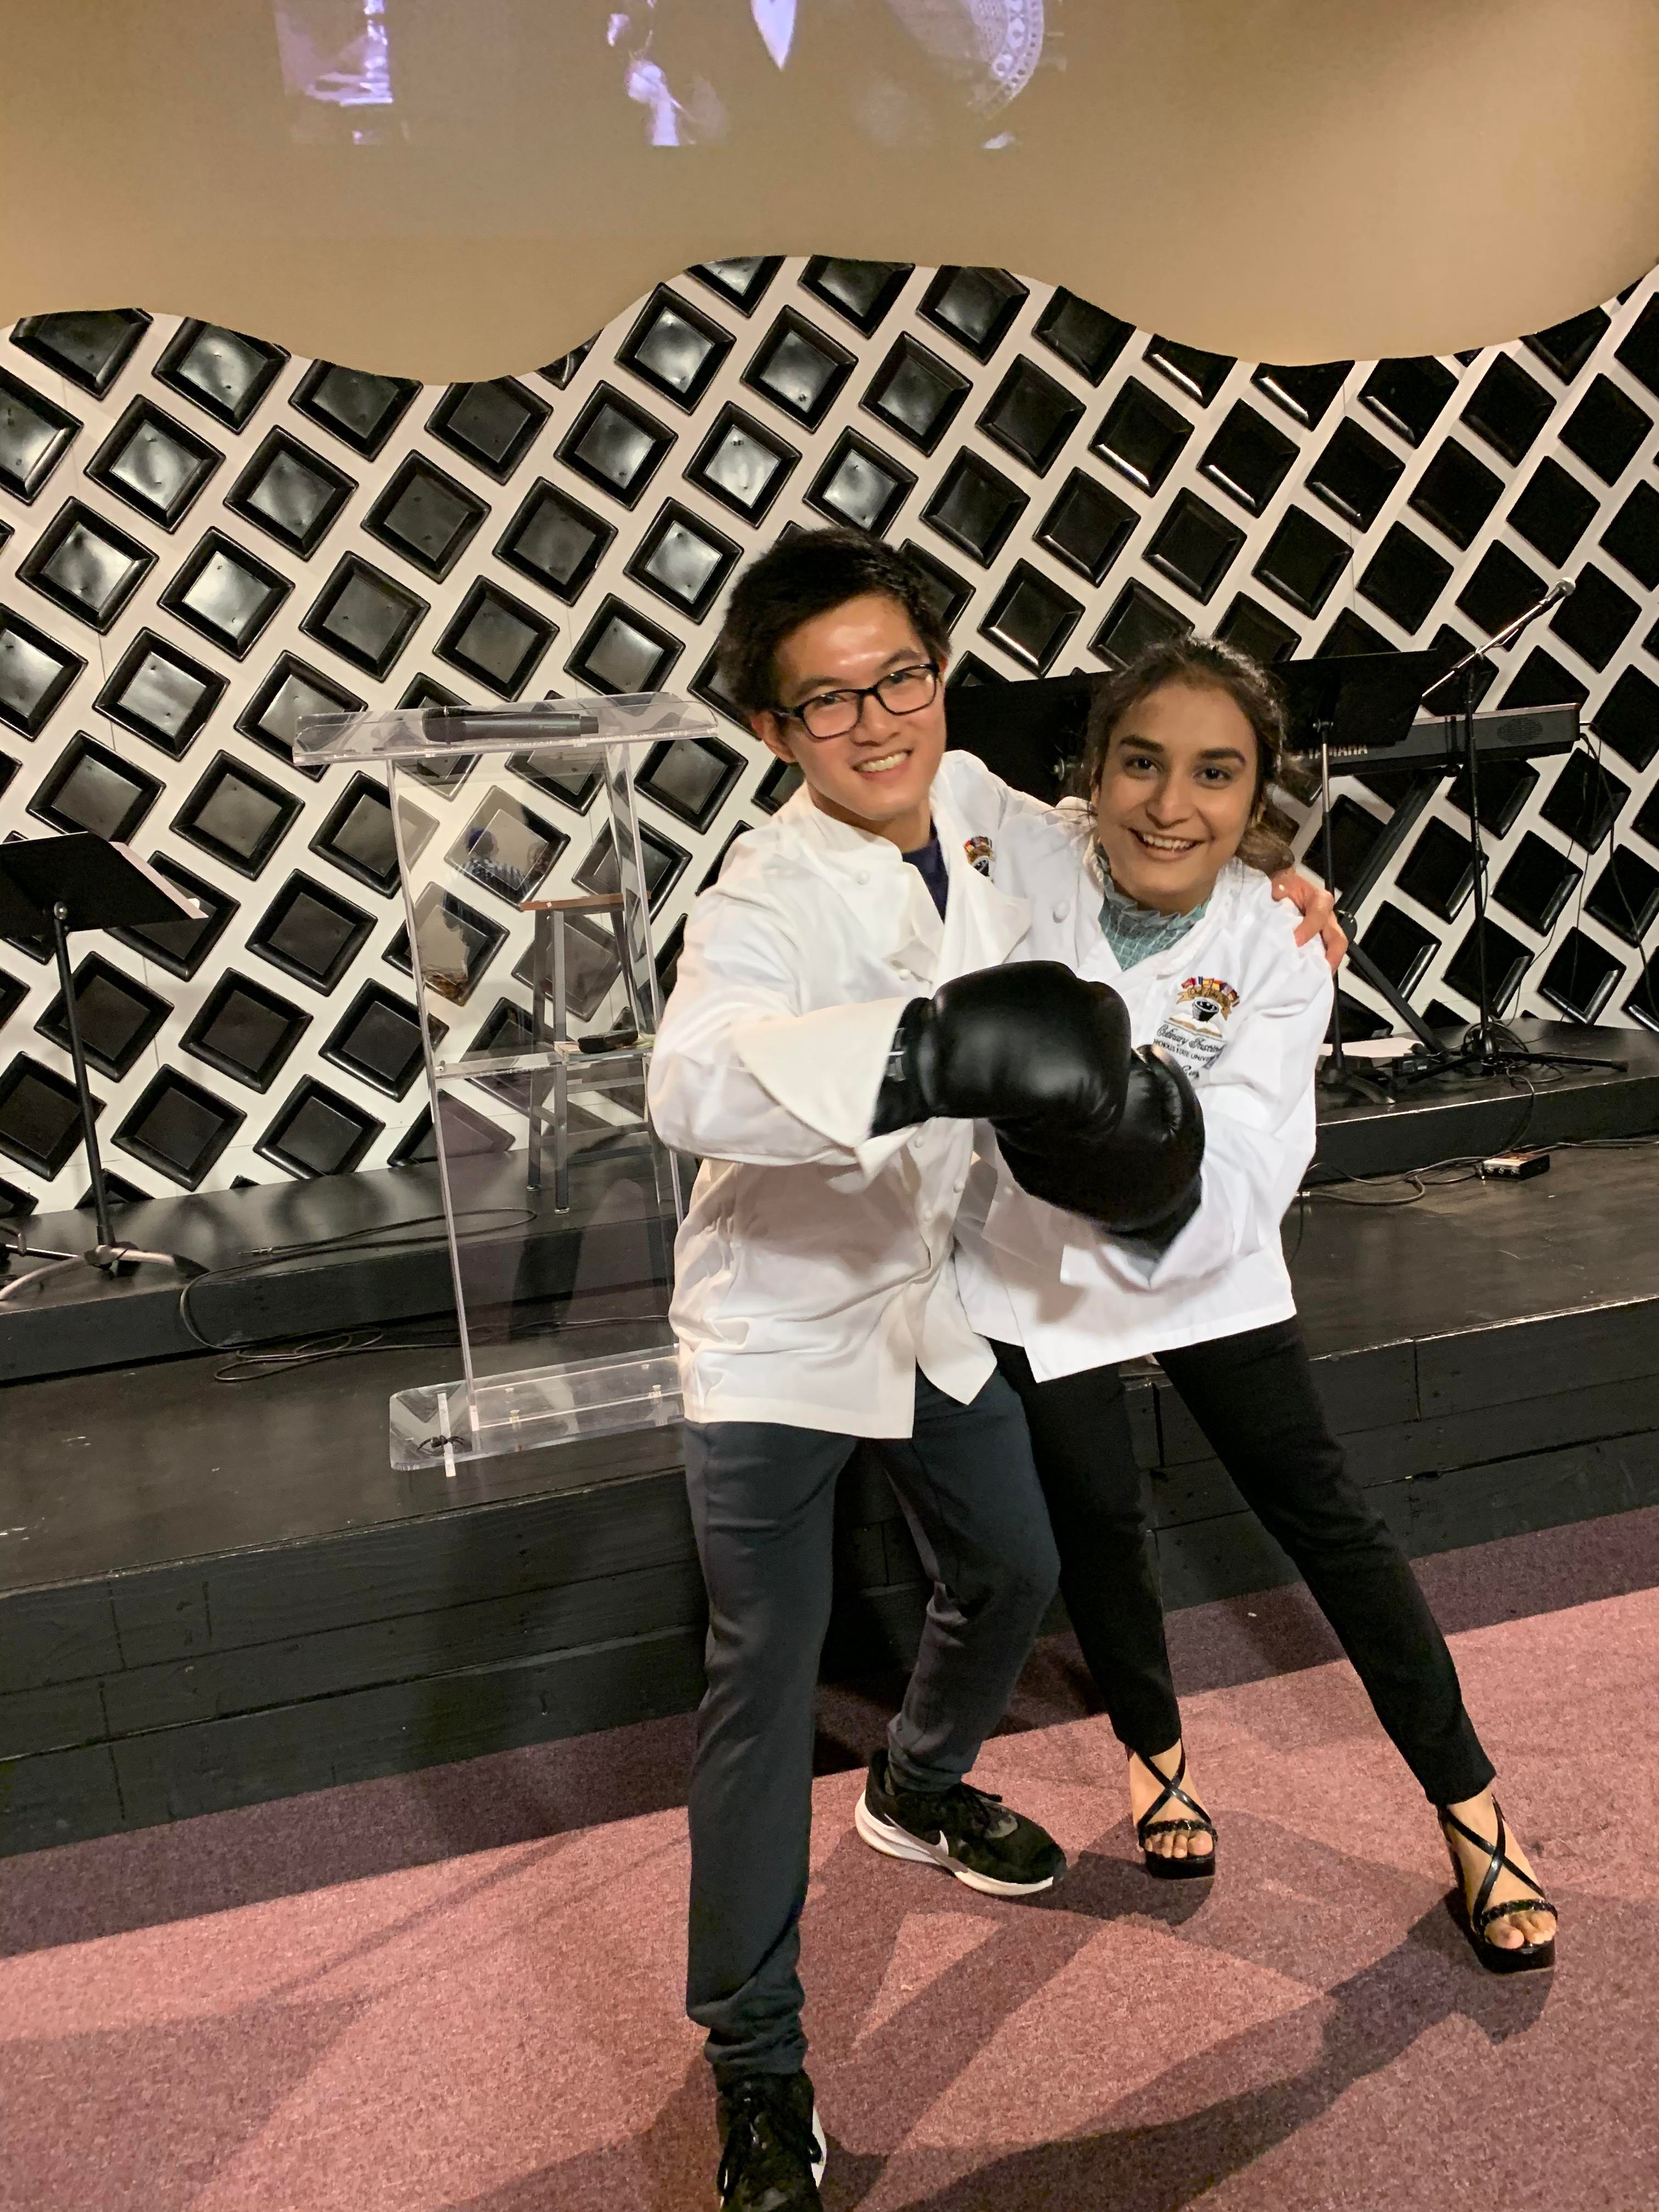
\includegraphics[width=5.20833in,height=\textheight]{mimages/4 10-30-2020.jpg}
\caption{October 30, 2020}
\end{figure}

\begin{figure}
\centering
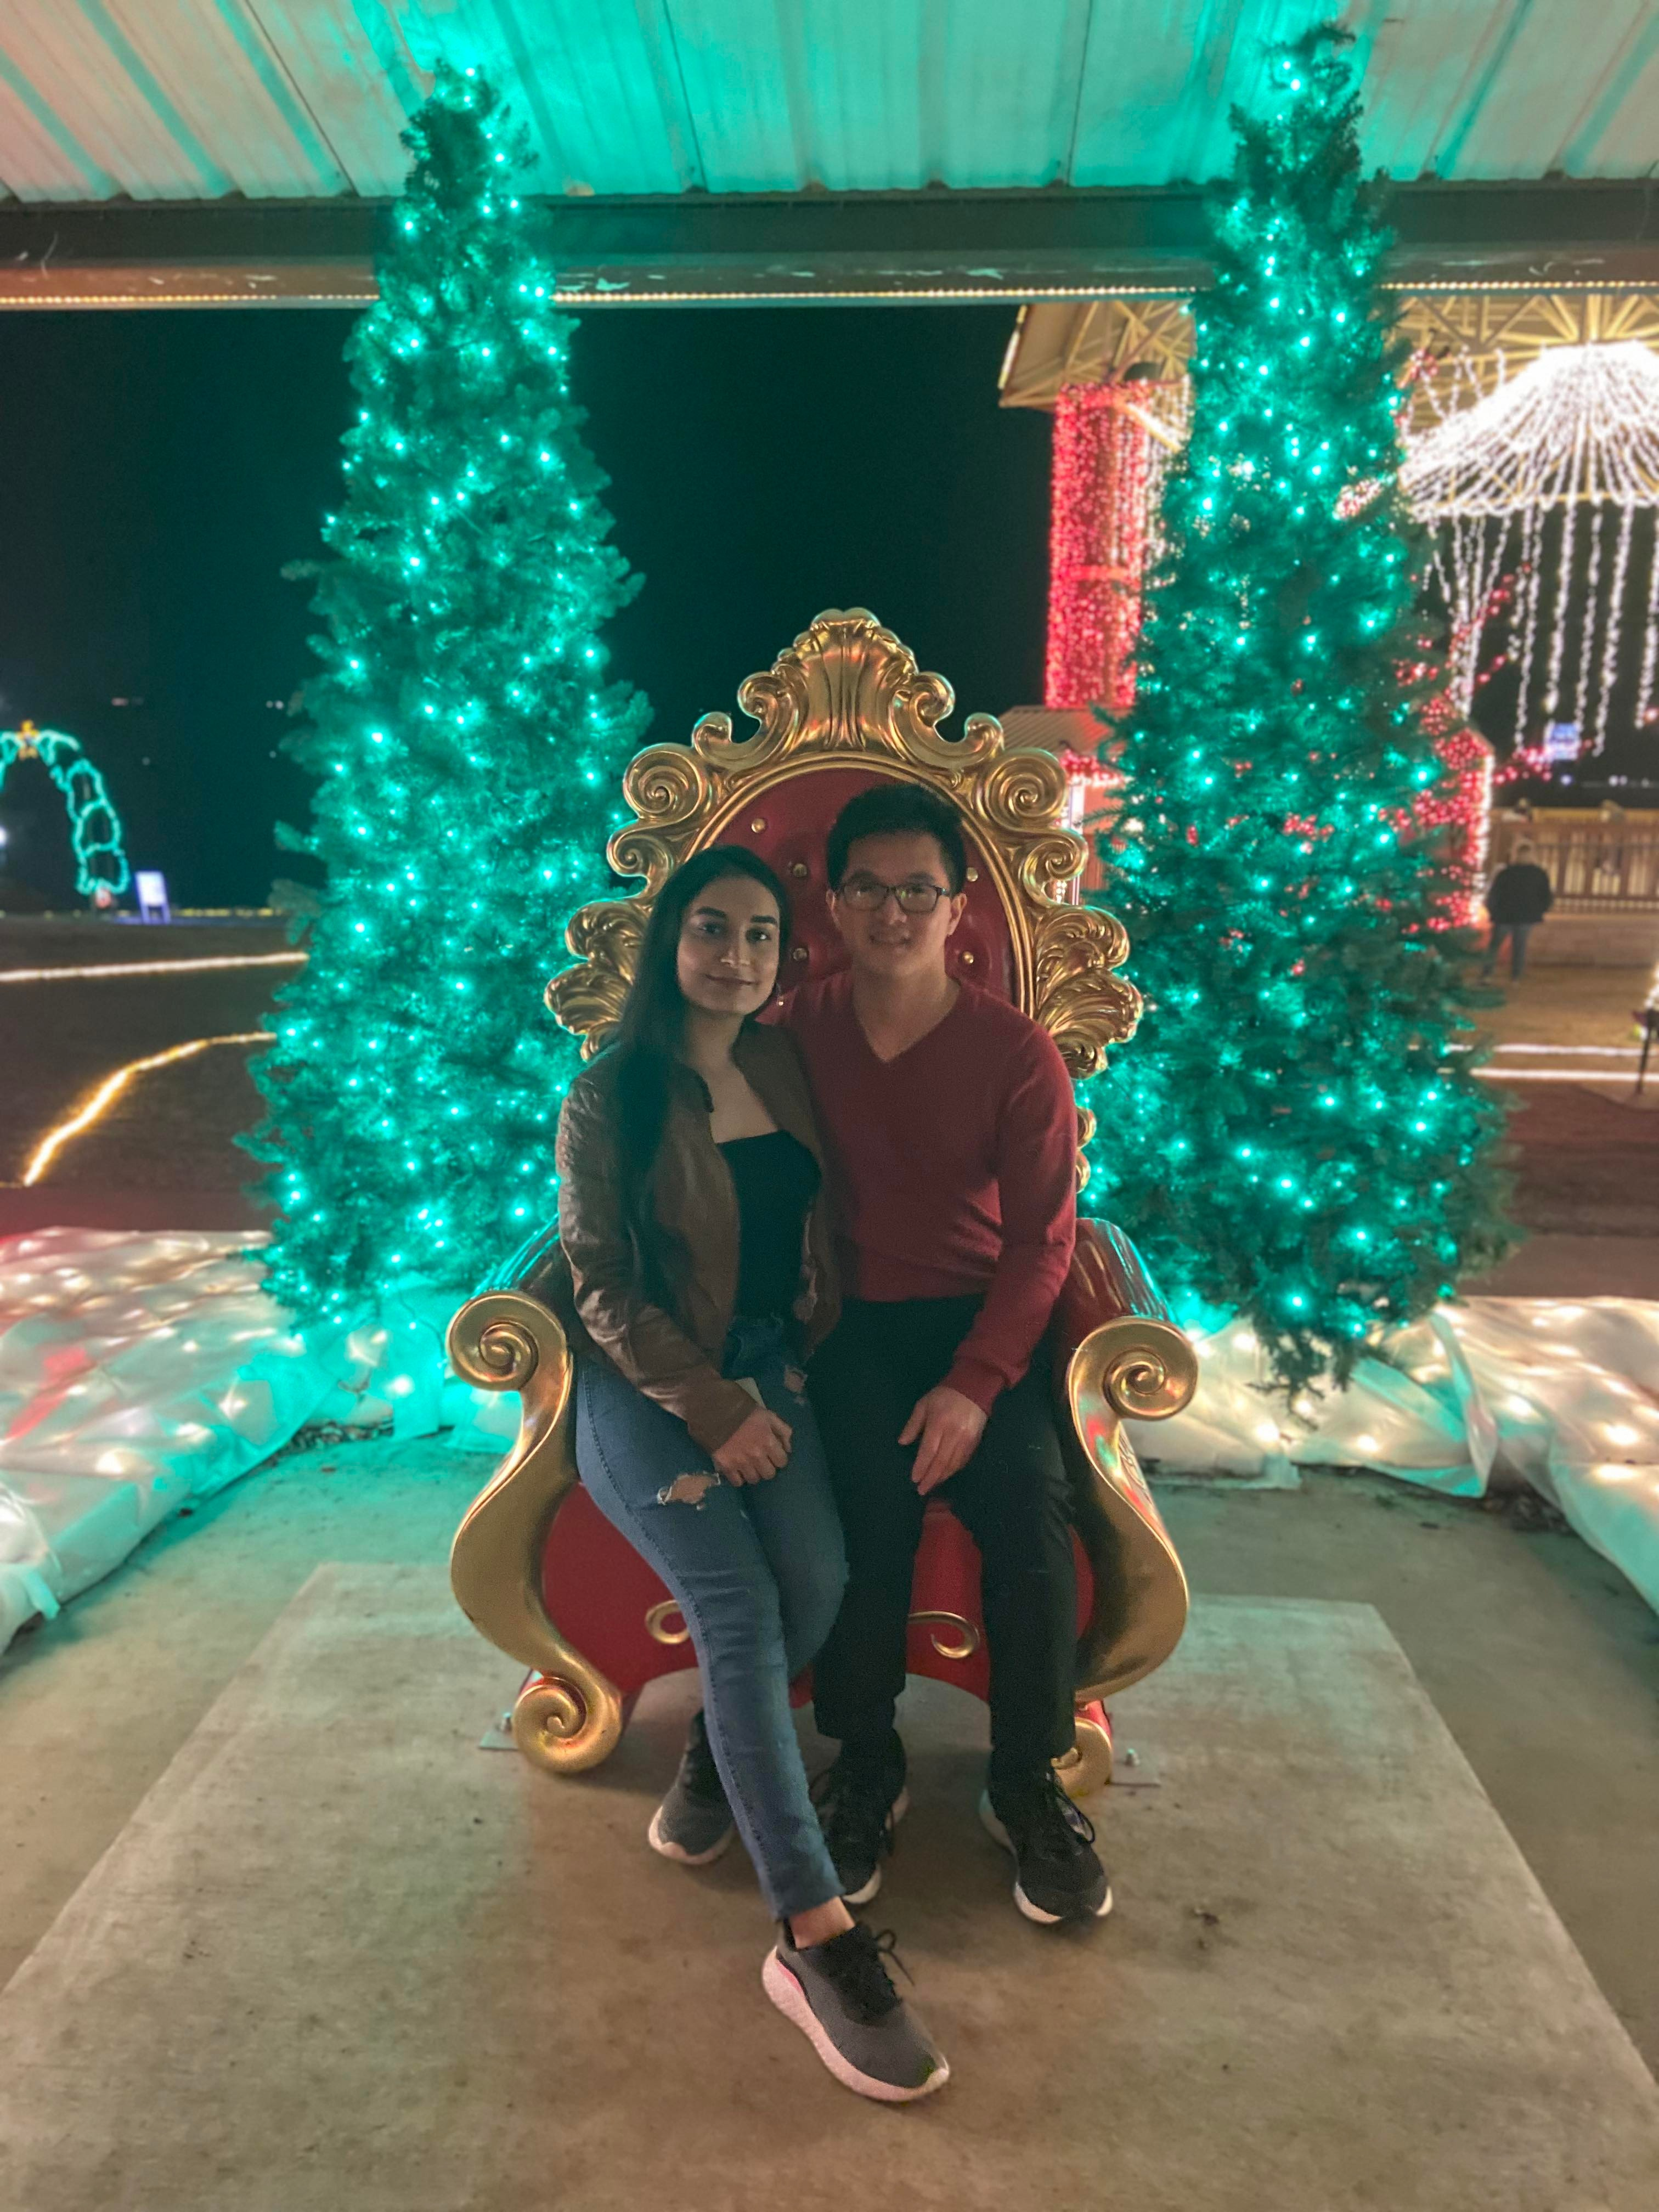
\includegraphics[width=5.20833in,height=\textheight]{mimages/14 12-24-2021.jpg}
\caption{December 24, 2021}
\end{figure}

\begin{figure}
\centering
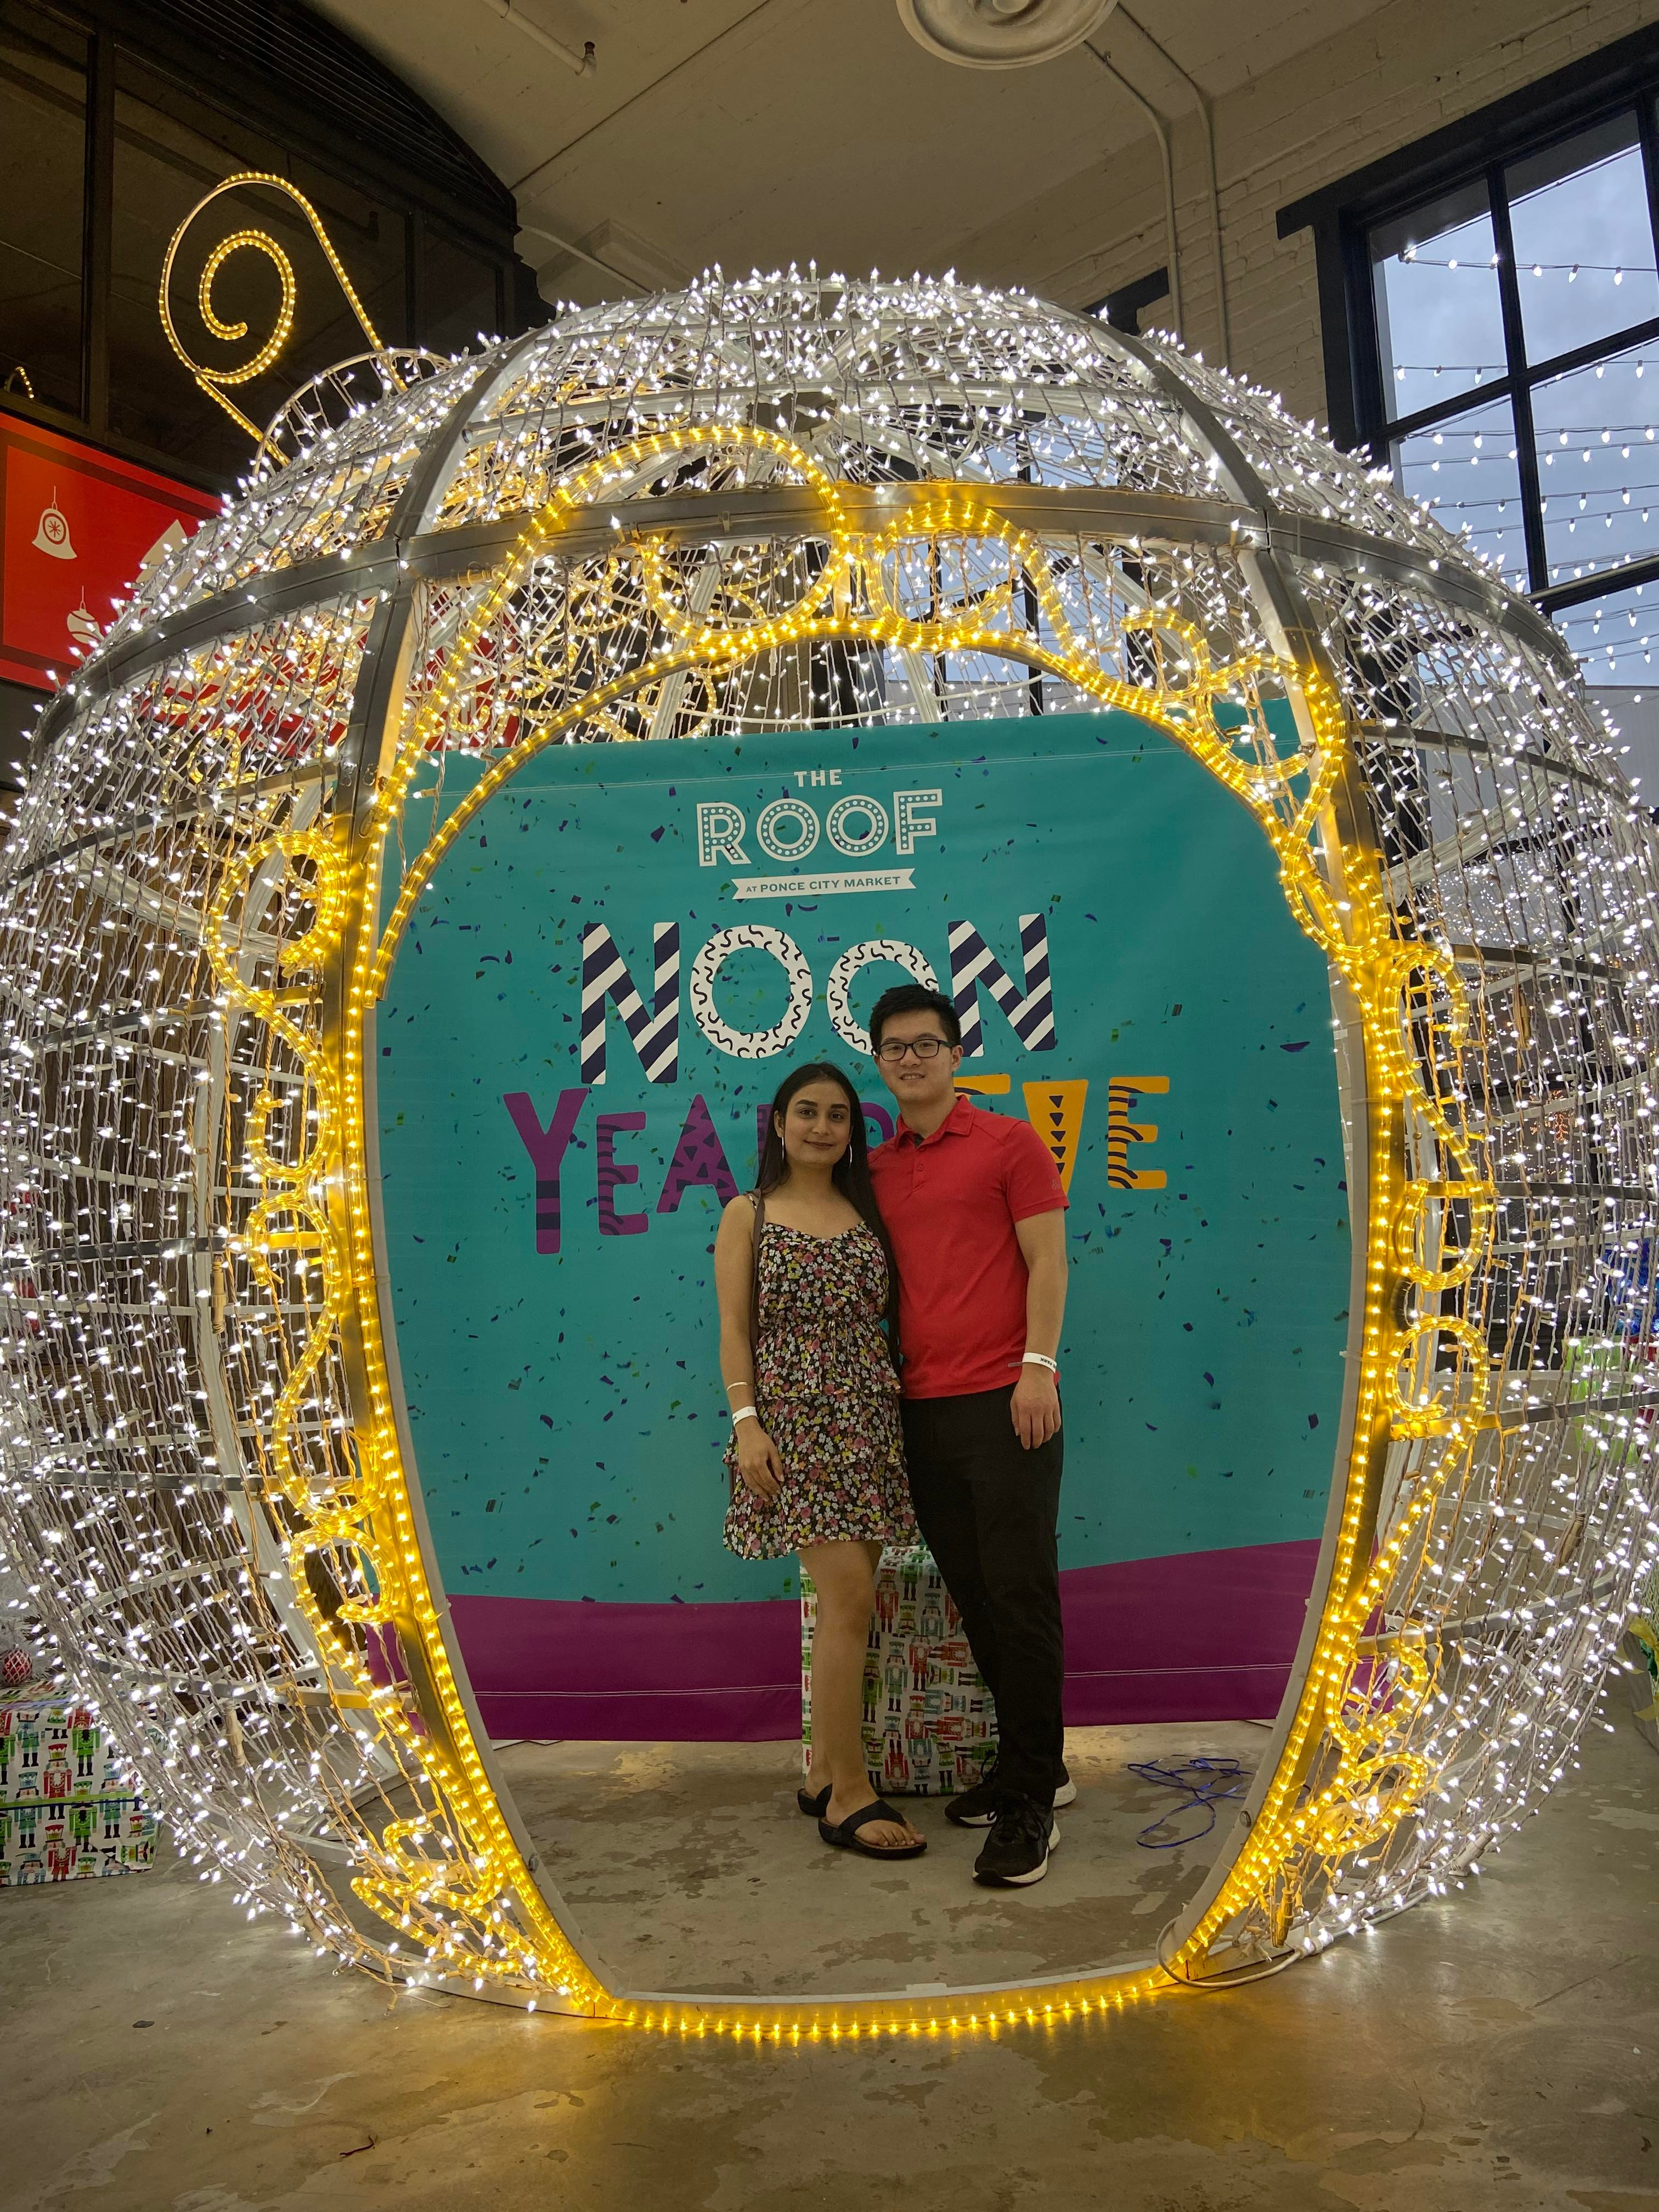
\includegraphics[width=5.20833in,height=\textheight]{mimages/15 12-31-2021.jpg}
\caption{December 31, 2021}
\end{figure}

\hypertarget{sleepless-nights-house-alone}{%
\chapter{Sleepless Nights House Alone}\label{sleepless-nights-house-alone}}

\begin{Shaded}
\begin{Highlighting}[]
\NormalTok{I am older now.}
\NormalTok{Trained by parents.}
\NormalTok{But still protected by fear.}

\NormalTok{I sleep lightly,}
\NormalTok{Scared of something,}
\NormalTok{Stirred to uncertainty.}

\NormalTok{No laws against silence,}
\NormalTok{Every sound a nail,}
\NormalTok{to the boards of emptiness.}

\NormalTok{A frenzied attack.}
\NormalTok{I merely lie still,}
\NormalTok{With no means of defense.}

\NormalTok{How my skin crawls, itches, and senses,}
\NormalTok{The assault begins,}
\NormalTok{As I start my sleep.}

\NormalTok{Why do I let my mind,}
\NormalTok{Premature }\ControlFlowTok{in}\NormalTok{ sleep.}
\NormalTok{Get under my skin.}

\NormalTok{How I wish to take shelter }\ControlFlowTok{in}\NormalTok{ you.}
\NormalTok{to hold you, to kiss you,}
\NormalTok{and stay by you forever.}
\end{Highlighting}
\end{Shaded}

\begin{figure}
\centering
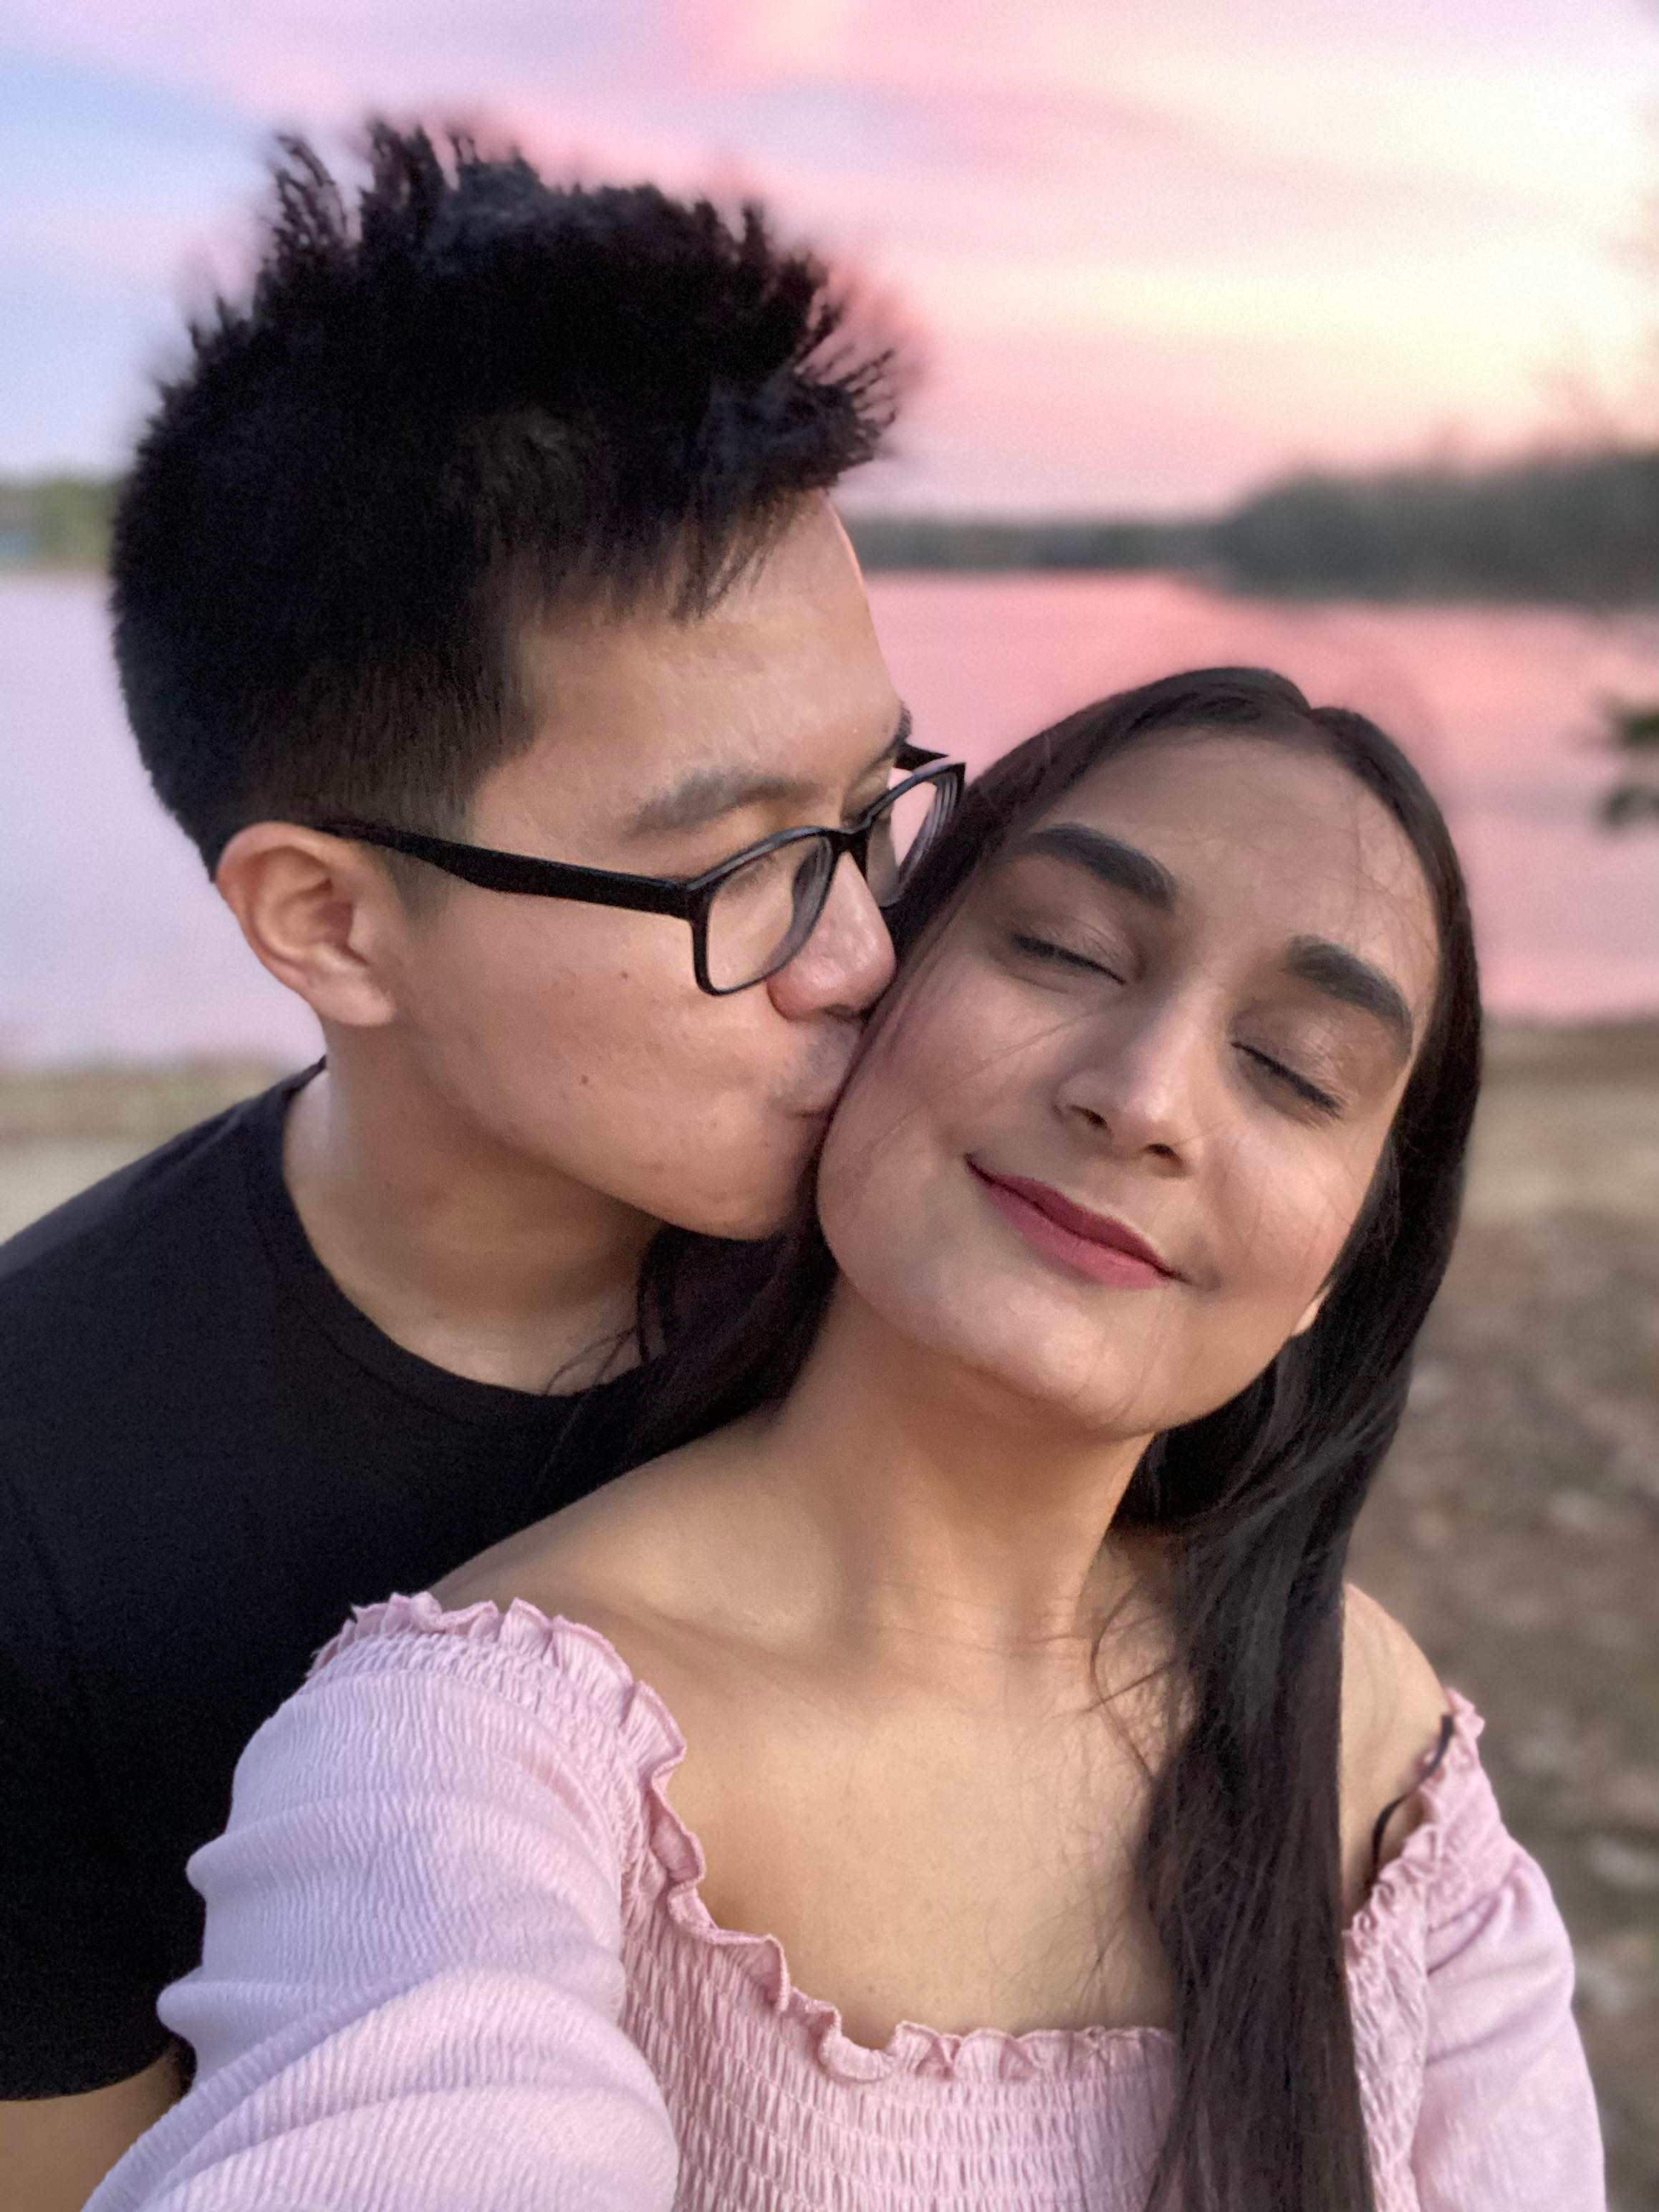
\includegraphics[width=5.20833in,height=\textheight]{mimages/14.1 12-24-2021.jpg}
\caption{December 24, 2021}
\end{figure}

\begin{figure}
\centering
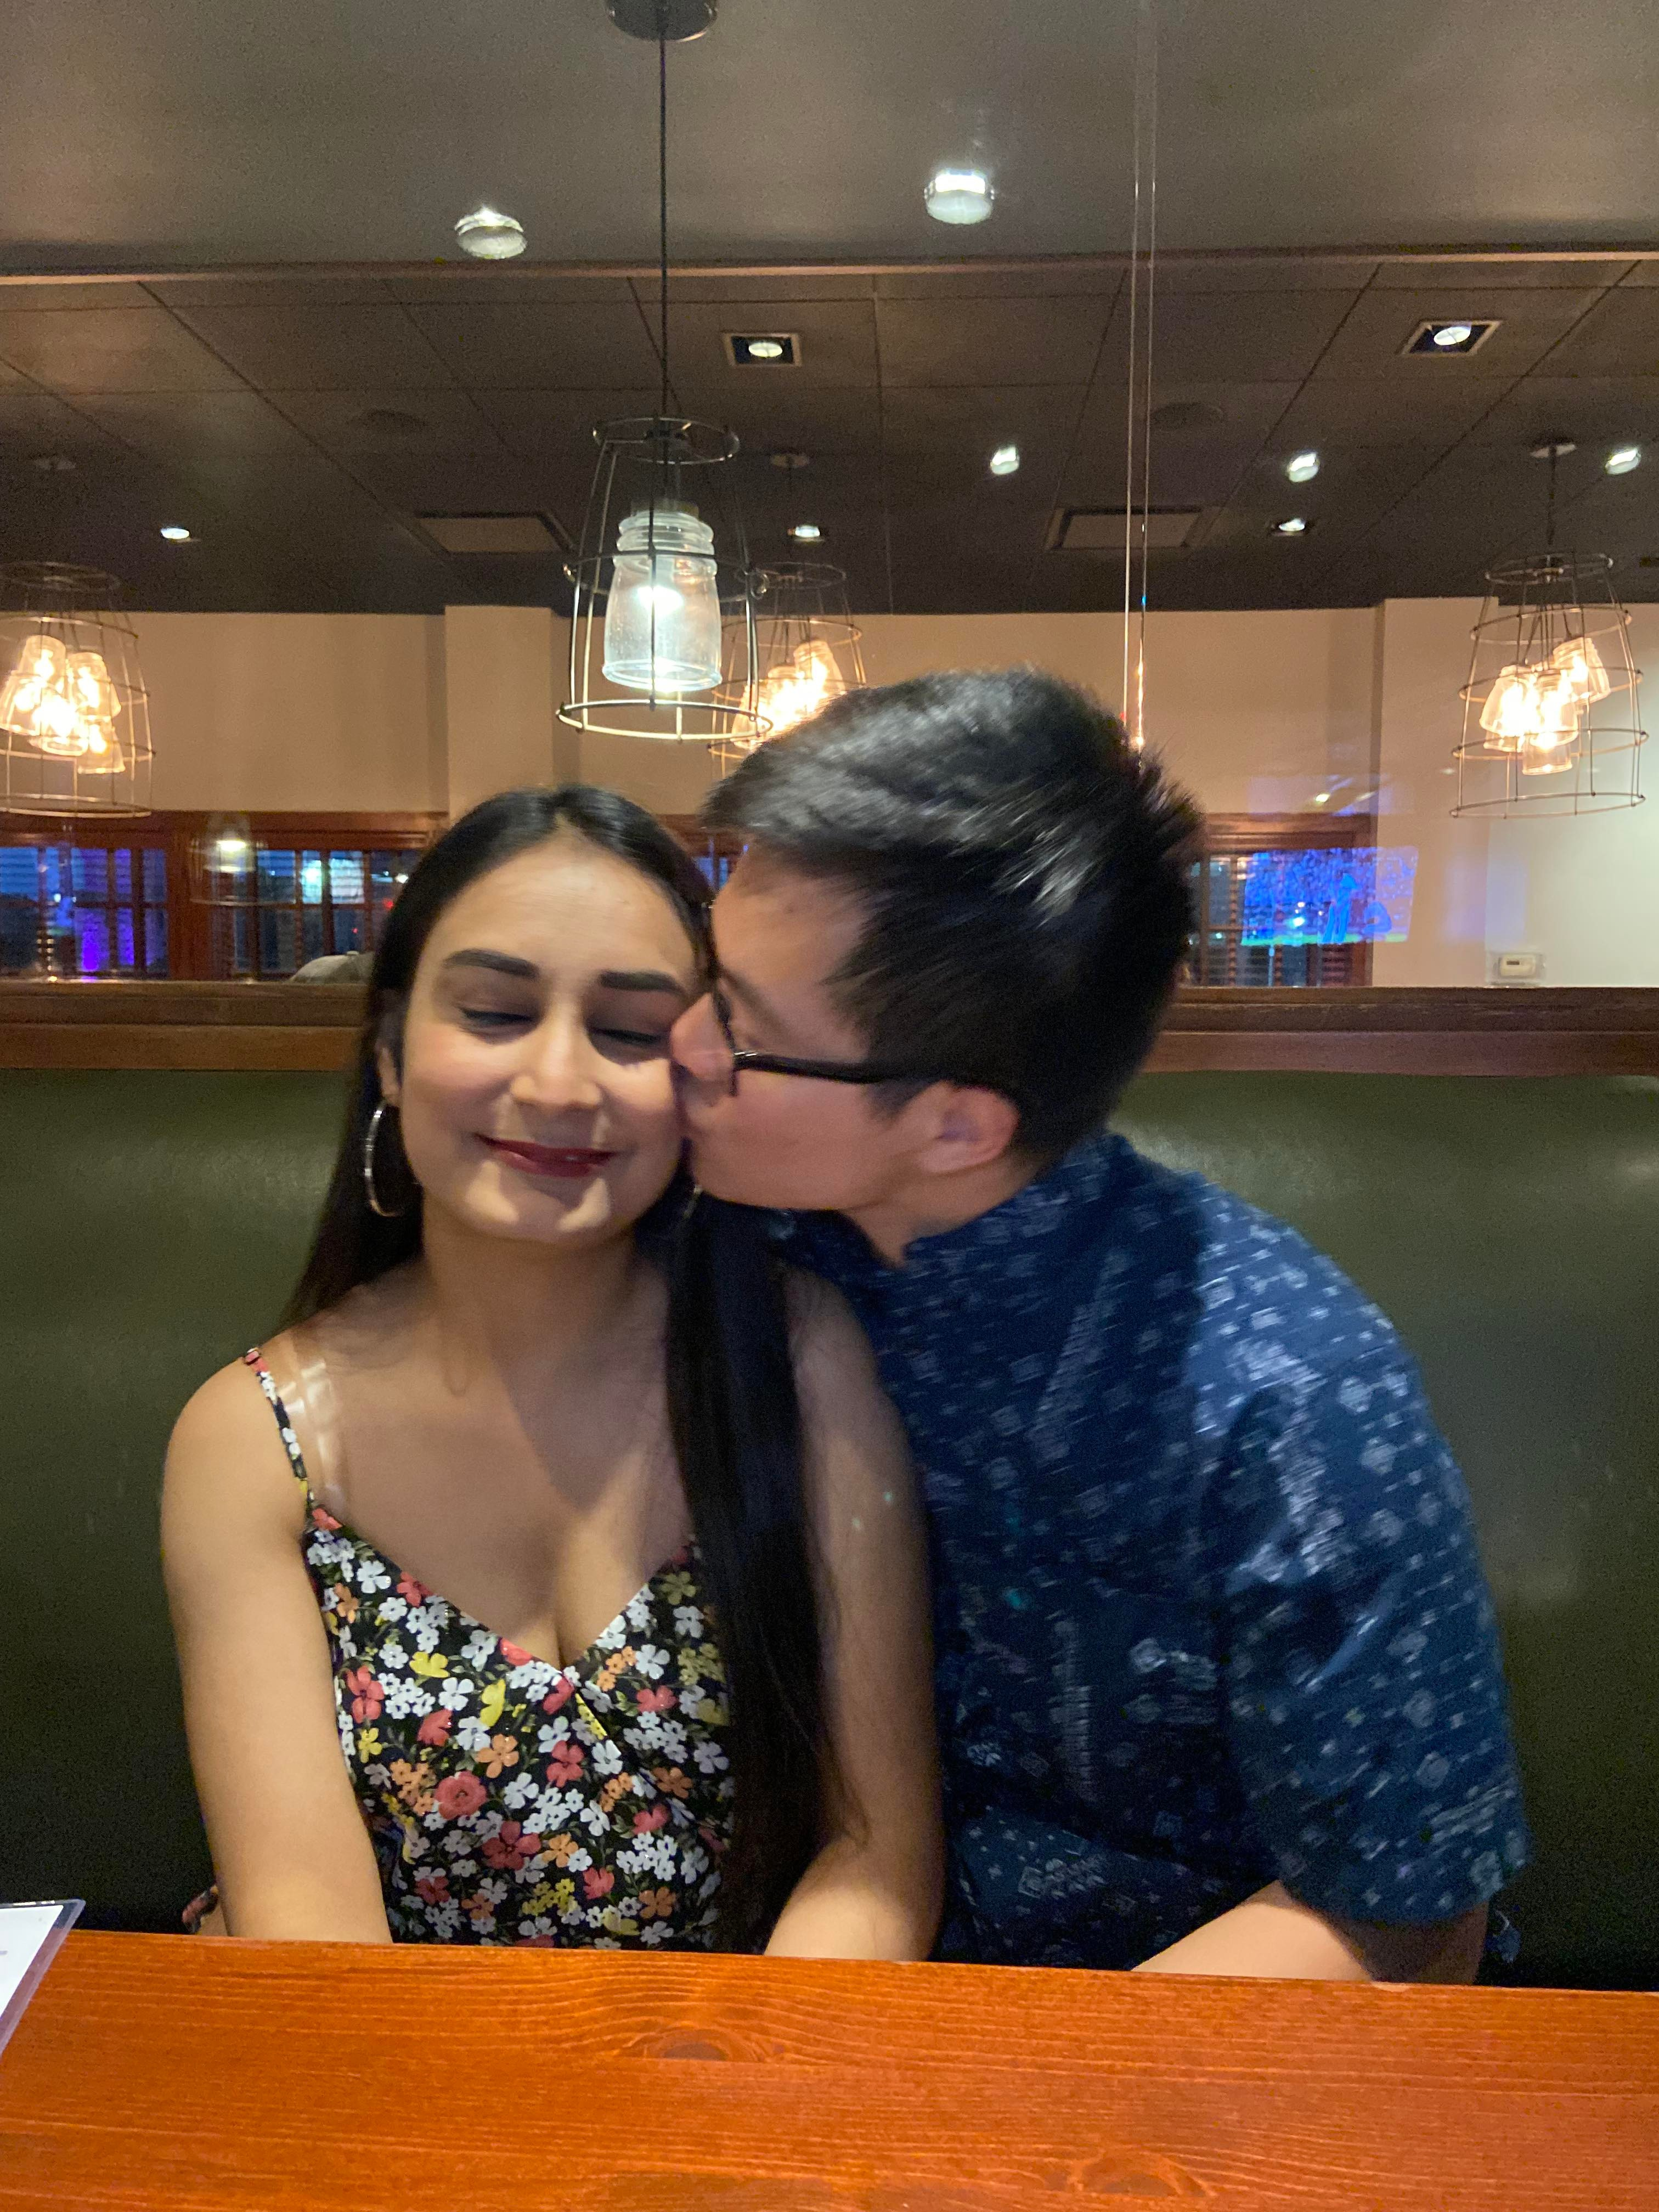
\includegraphics[width=5.20833in,height=\textheight]{mimages/13.1 9-11-2021.jpg}
\caption{September 11, 2021}
\end{figure}

\begin{figure}
\centering
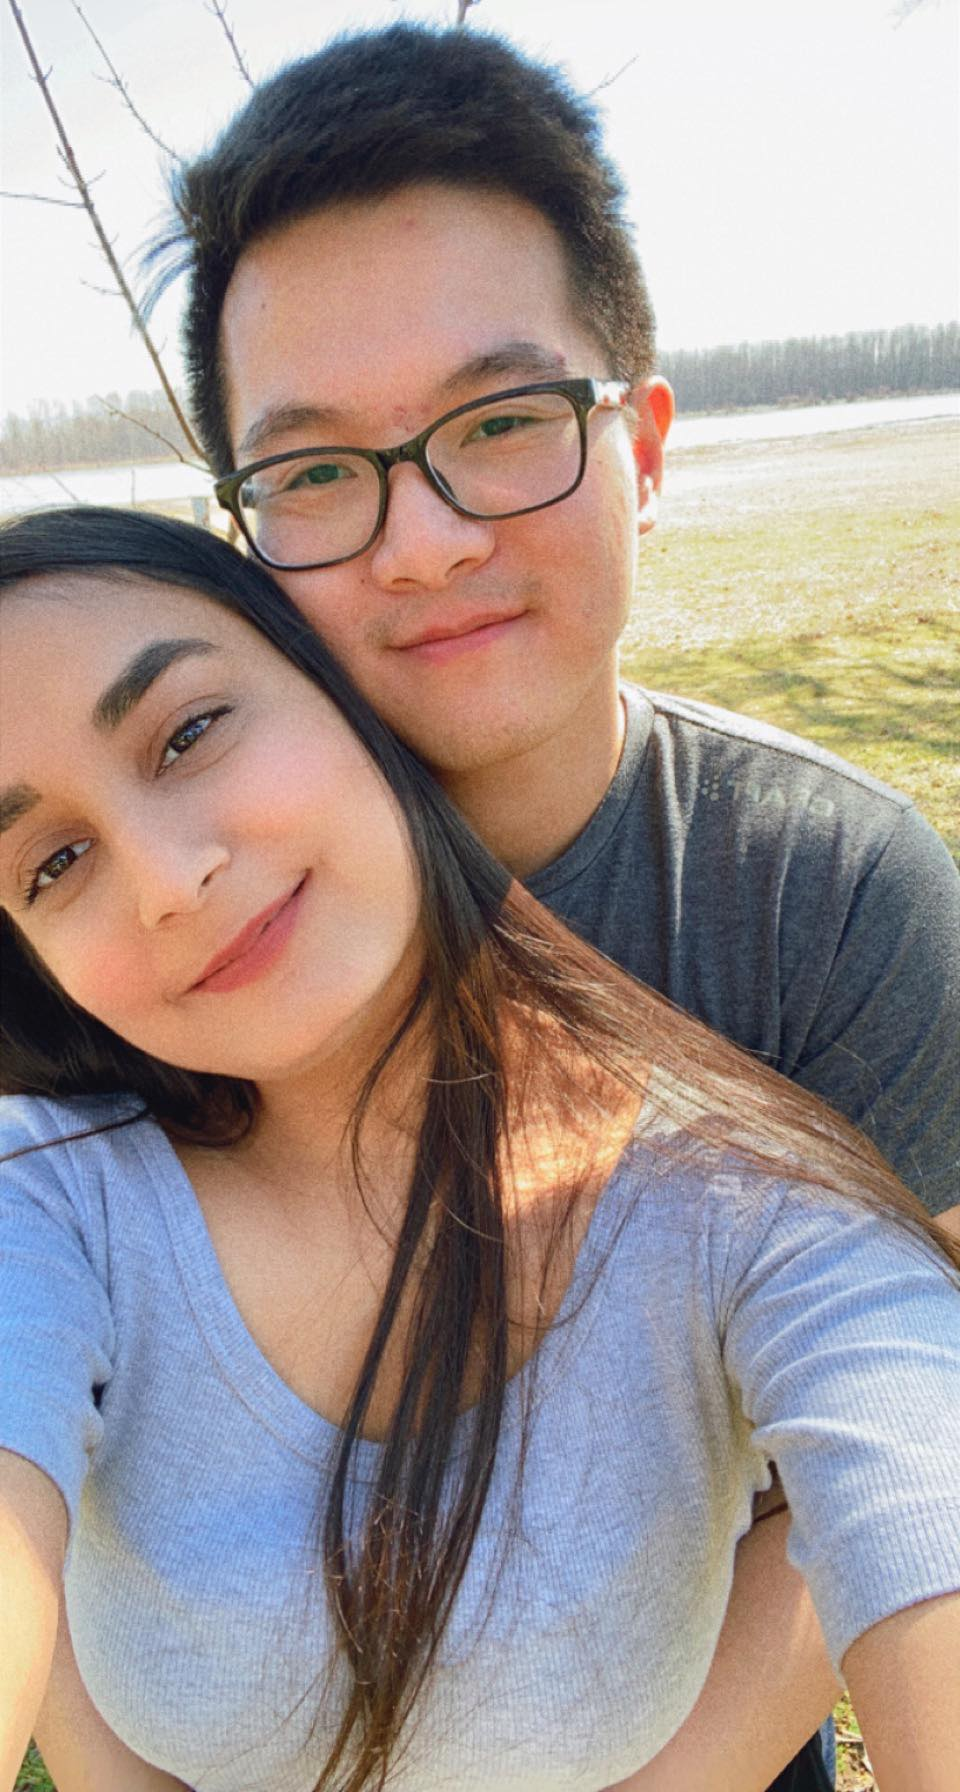
\includegraphics[width=5.20833in,height=\textheight]{mimages/17 3-16-2022.jpg}
\caption{March 16, 2022}
\end{figure}

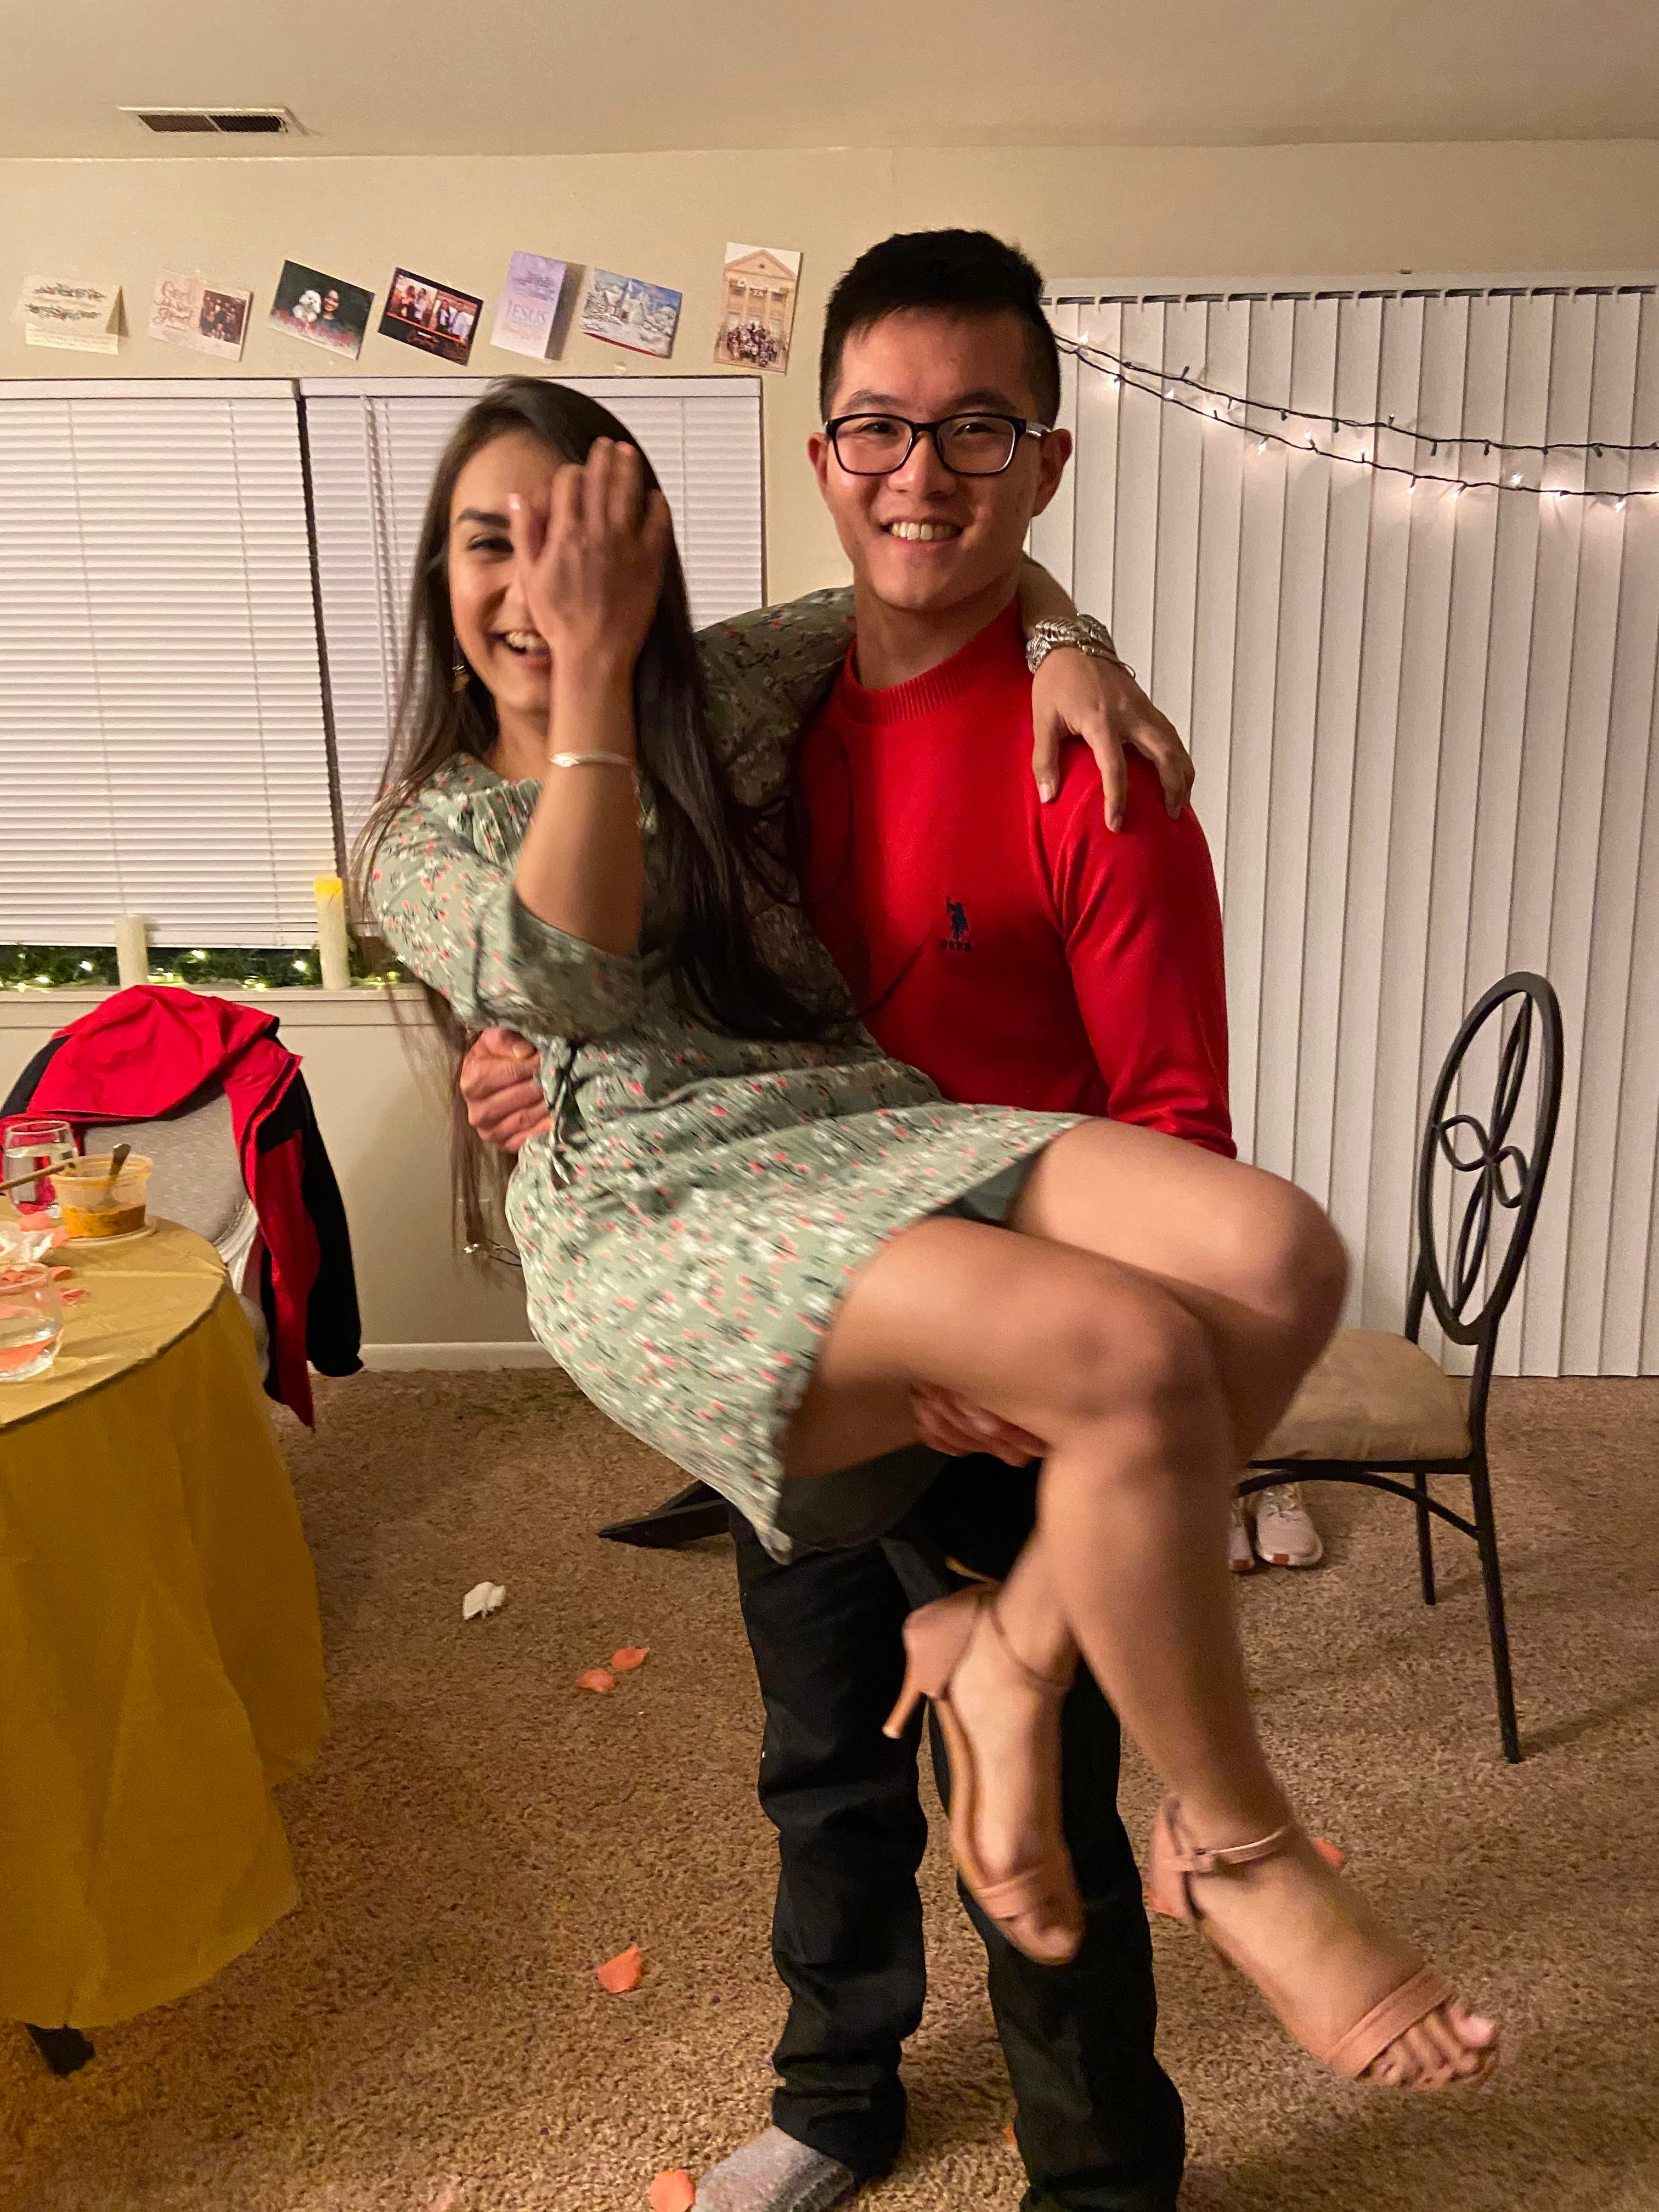
\includegraphics[width=5.20833in,height=\textheight]{mimages/7 2-16-2021.jpg}

\includegraphics[width=5.20833in,height=\textheight]{mimages/8.2 4-23-2021.jpg}

\hypertarget{journey}{%
\chapter{Journey}\label{journey}}

\begin{Shaded}
\begin{Highlighting}[]
\NormalTok{My hands on my fat thighs,}
\NormalTok{Believing I would end up lost.}
\NormalTok{My body signals,}
\NormalTok{Enough of this cruelty.}

\NormalTok{How I walk slowly back home,}
\NormalTok{Close to falling,}
\NormalTok{Sinking lower at each stride,}
\NormalTok{Rising high with each low.}

\NormalTok{Thousands of fools,}
\NormalTok{Obsessed }\ControlFlowTok{in}\NormalTok{ their self}\SpecialCharTok{{-}}\NormalTok{destruction,}
\NormalTok{But that’s how the journey is,}
\NormalTok{The journey of love.}

\NormalTok{To bear the distant longing,}
\NormalTok{To bear sleepiness from endless talking,}
\NormalTok{To bear two different worlds,}
\NormalTok{Hoping on converging.}

\NormalTok{How I hold space }\ControlFlowTok{in}\NormalTok{ my life,}
\NormalTok{For a vision of you,}
\NormalTok{Who will come by,}
\NormalTok{To lift me higher.}

\NormalTok{To feel a bond,}
\NormalTok{That feeling is }
\NormalTok{What I starve }\ControlFlowTok{for}
\NormalTok{Beyond all.}
\end{Highlighting}
\end{Shaded}

\begin{figure}
\centering
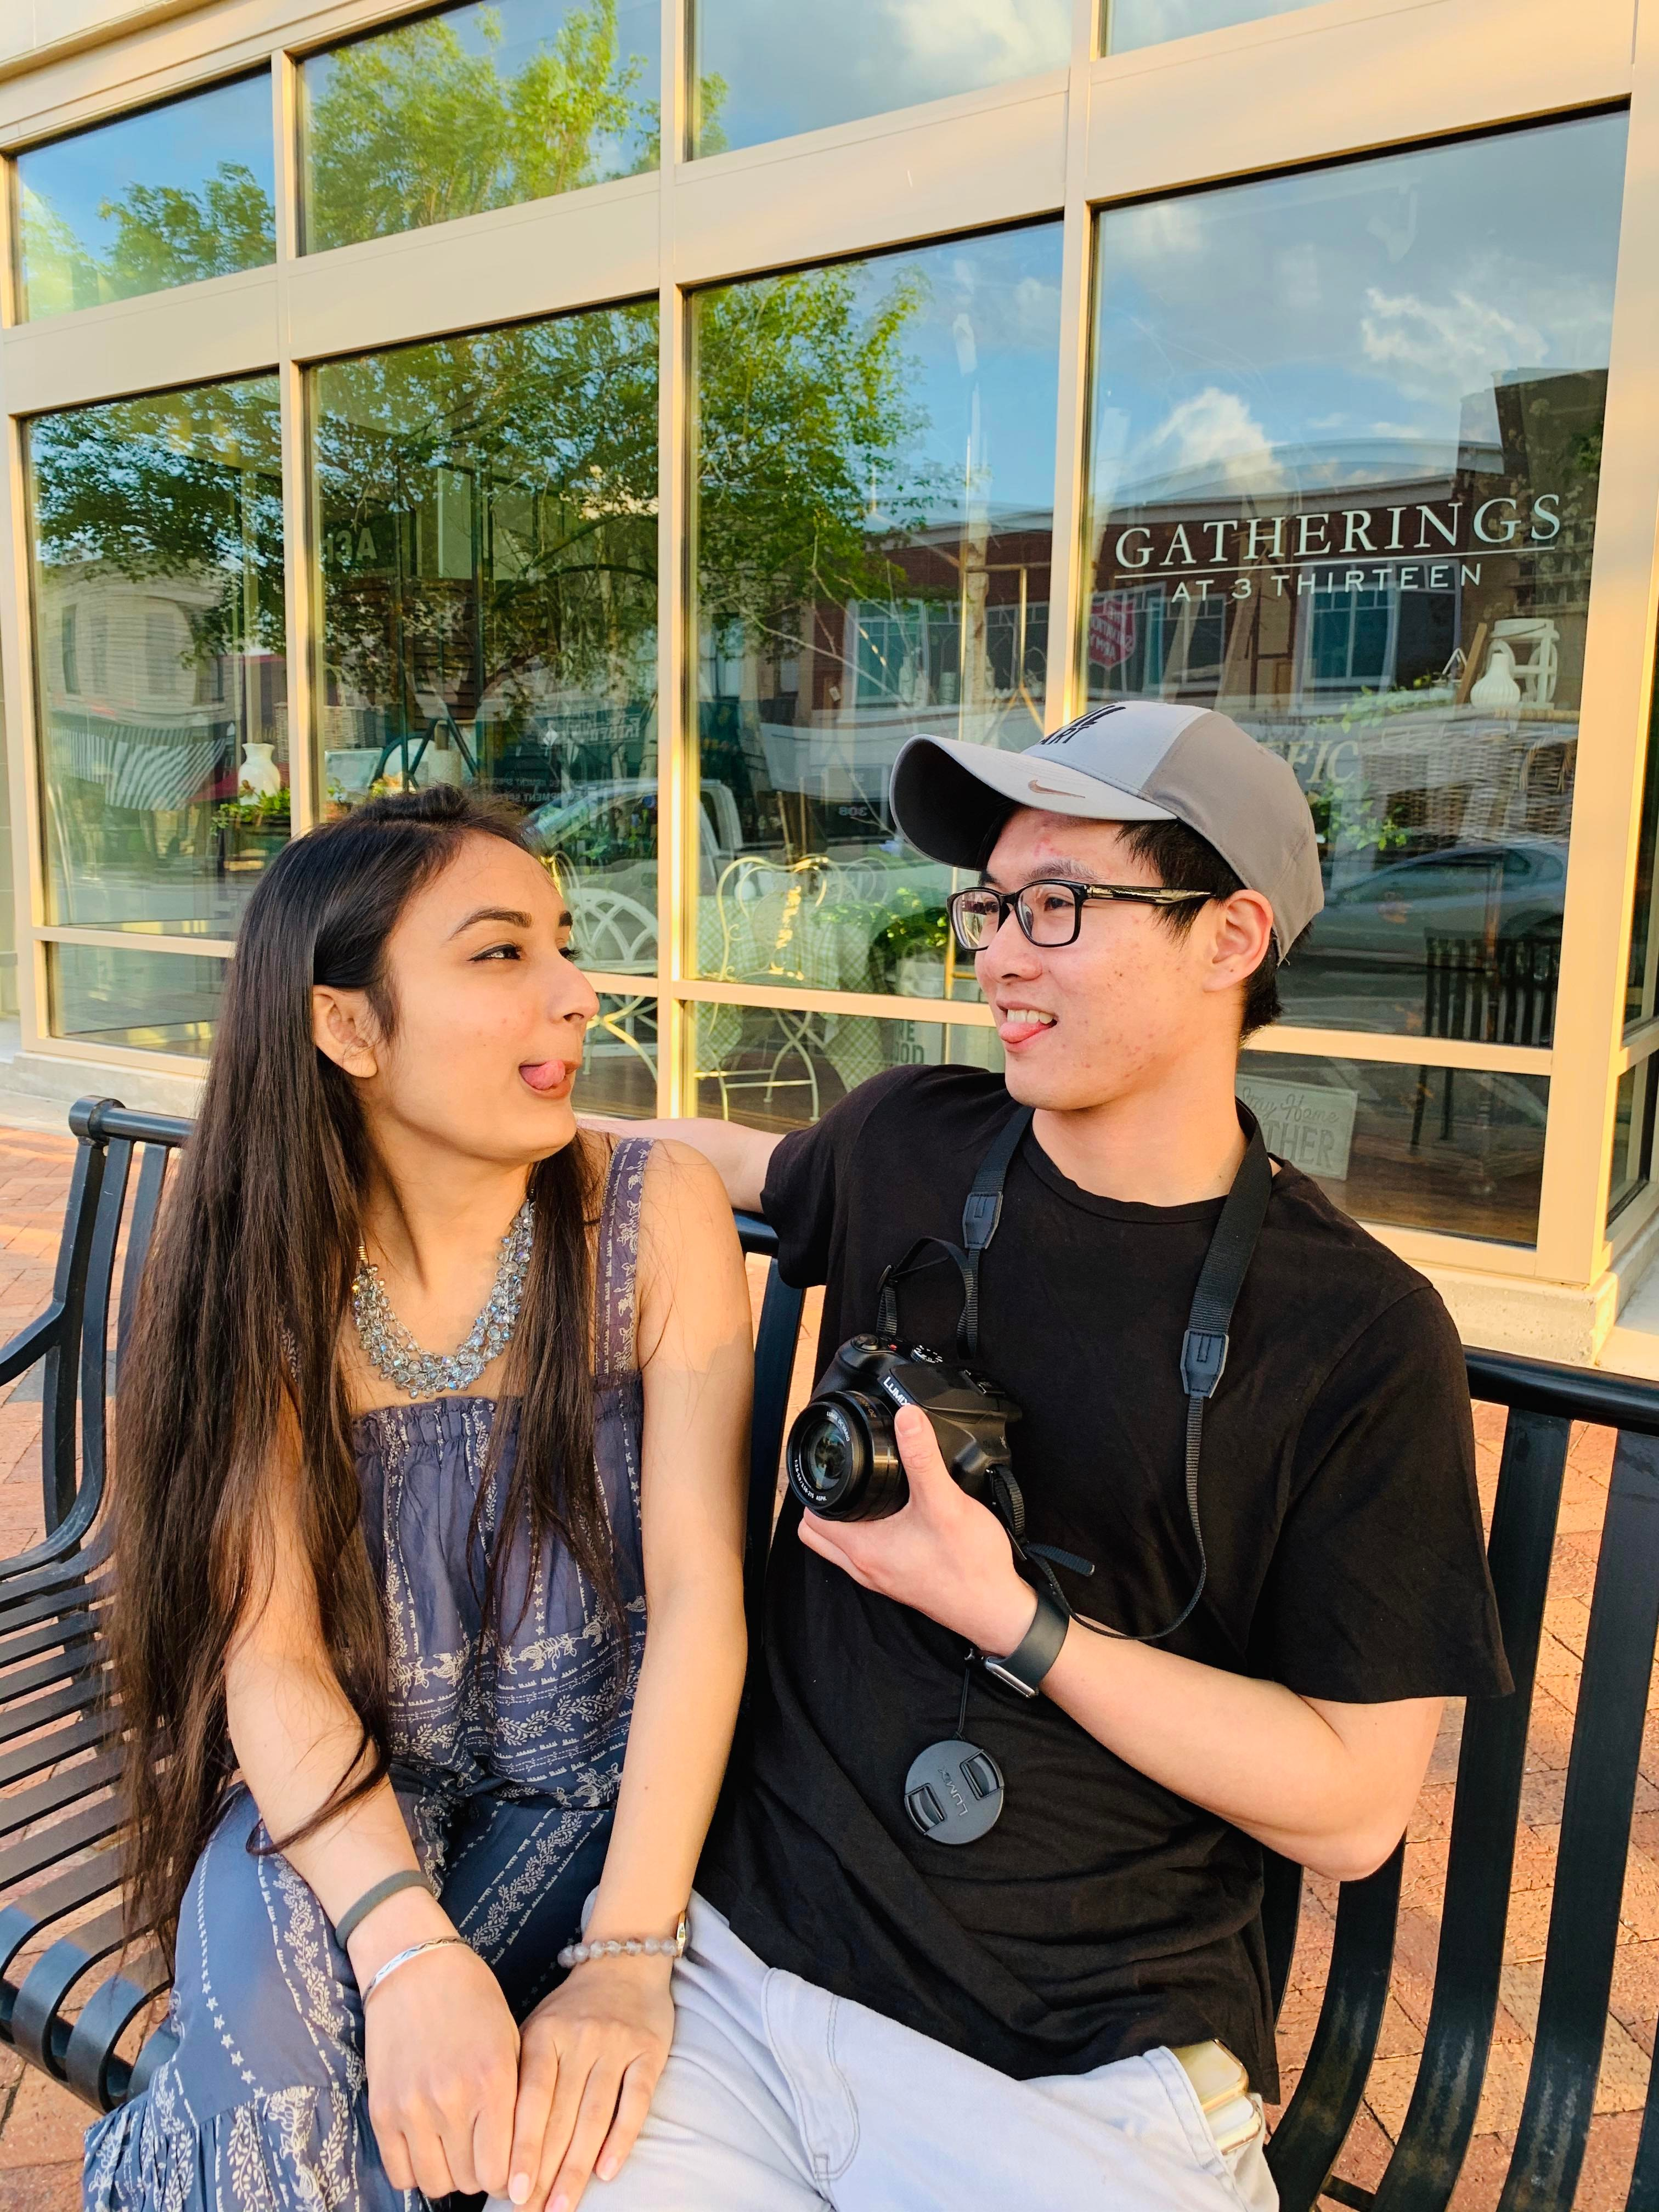
\includegraphics[width=5.20833in,height=\textheight]{mimages/0.1 4-25-2020.jpg}
\caption{April 25, 2020}
\end{figure}

\begin{figure}
\centering
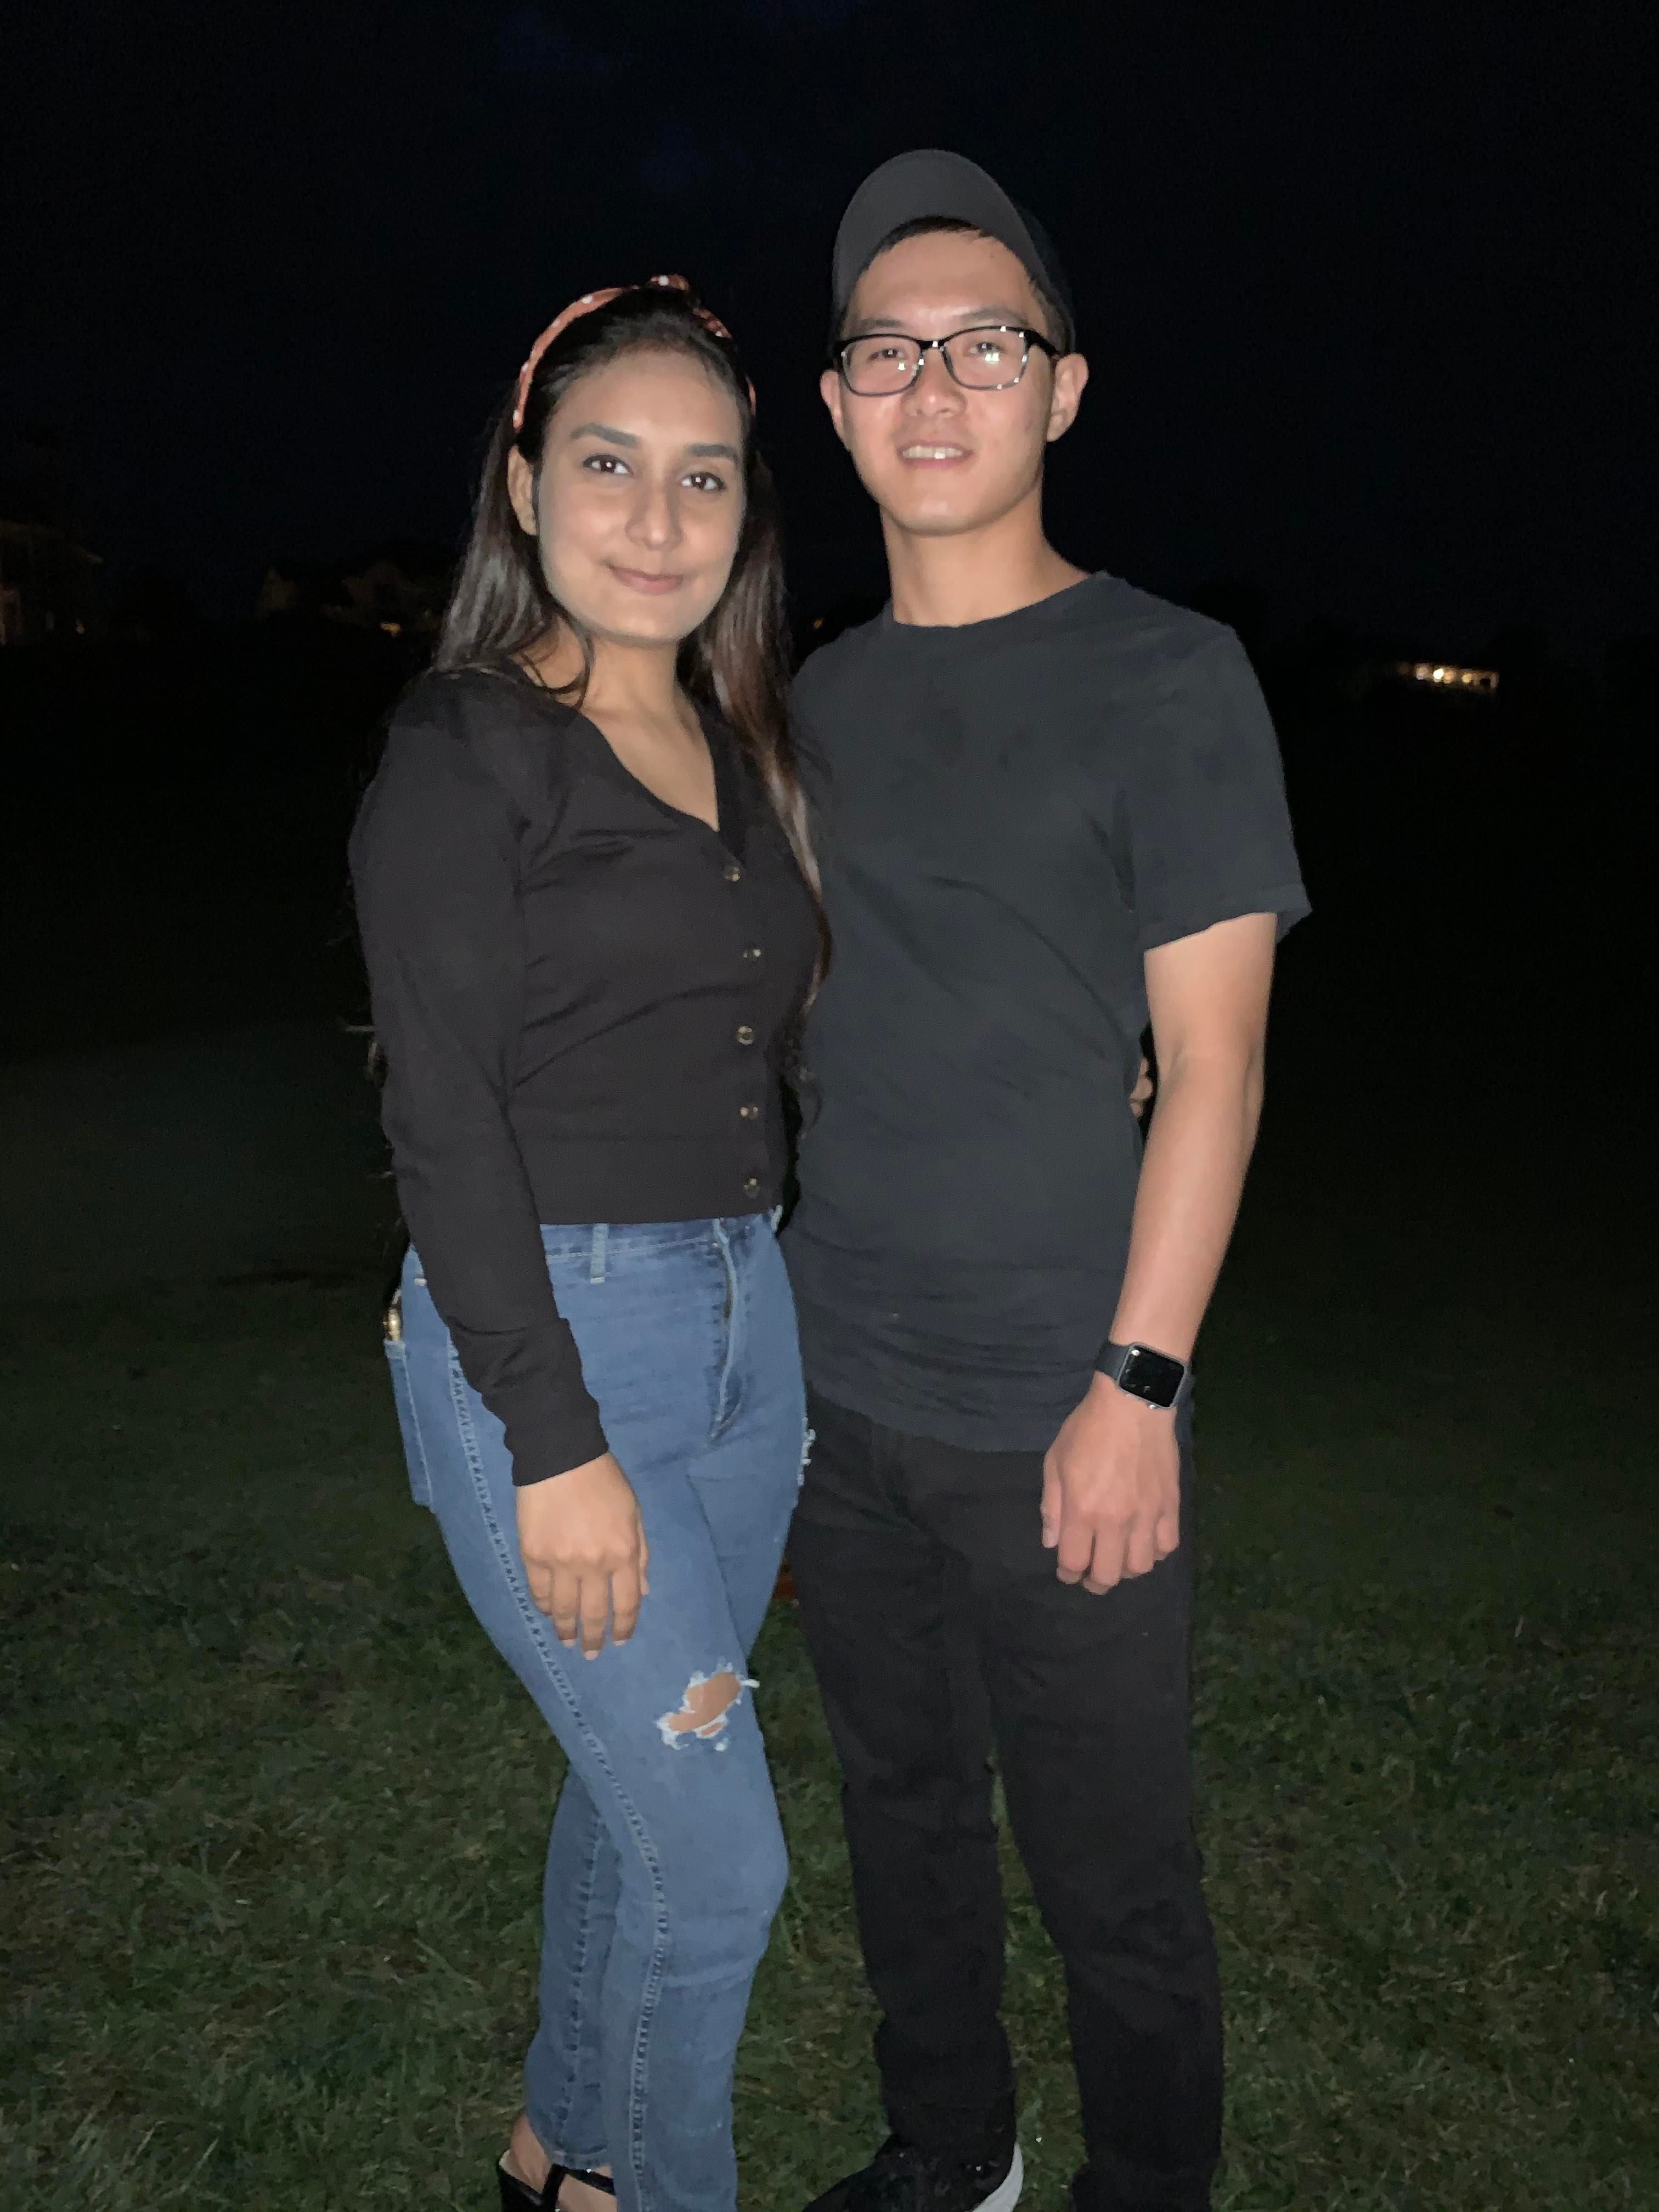
\includegraphics[width=5.20833in,height=\textheight]{mimages/3 9-11-2020.jpg}
\caption{September 11, 2020}
\end{figure}

\begin{figure}
\centering
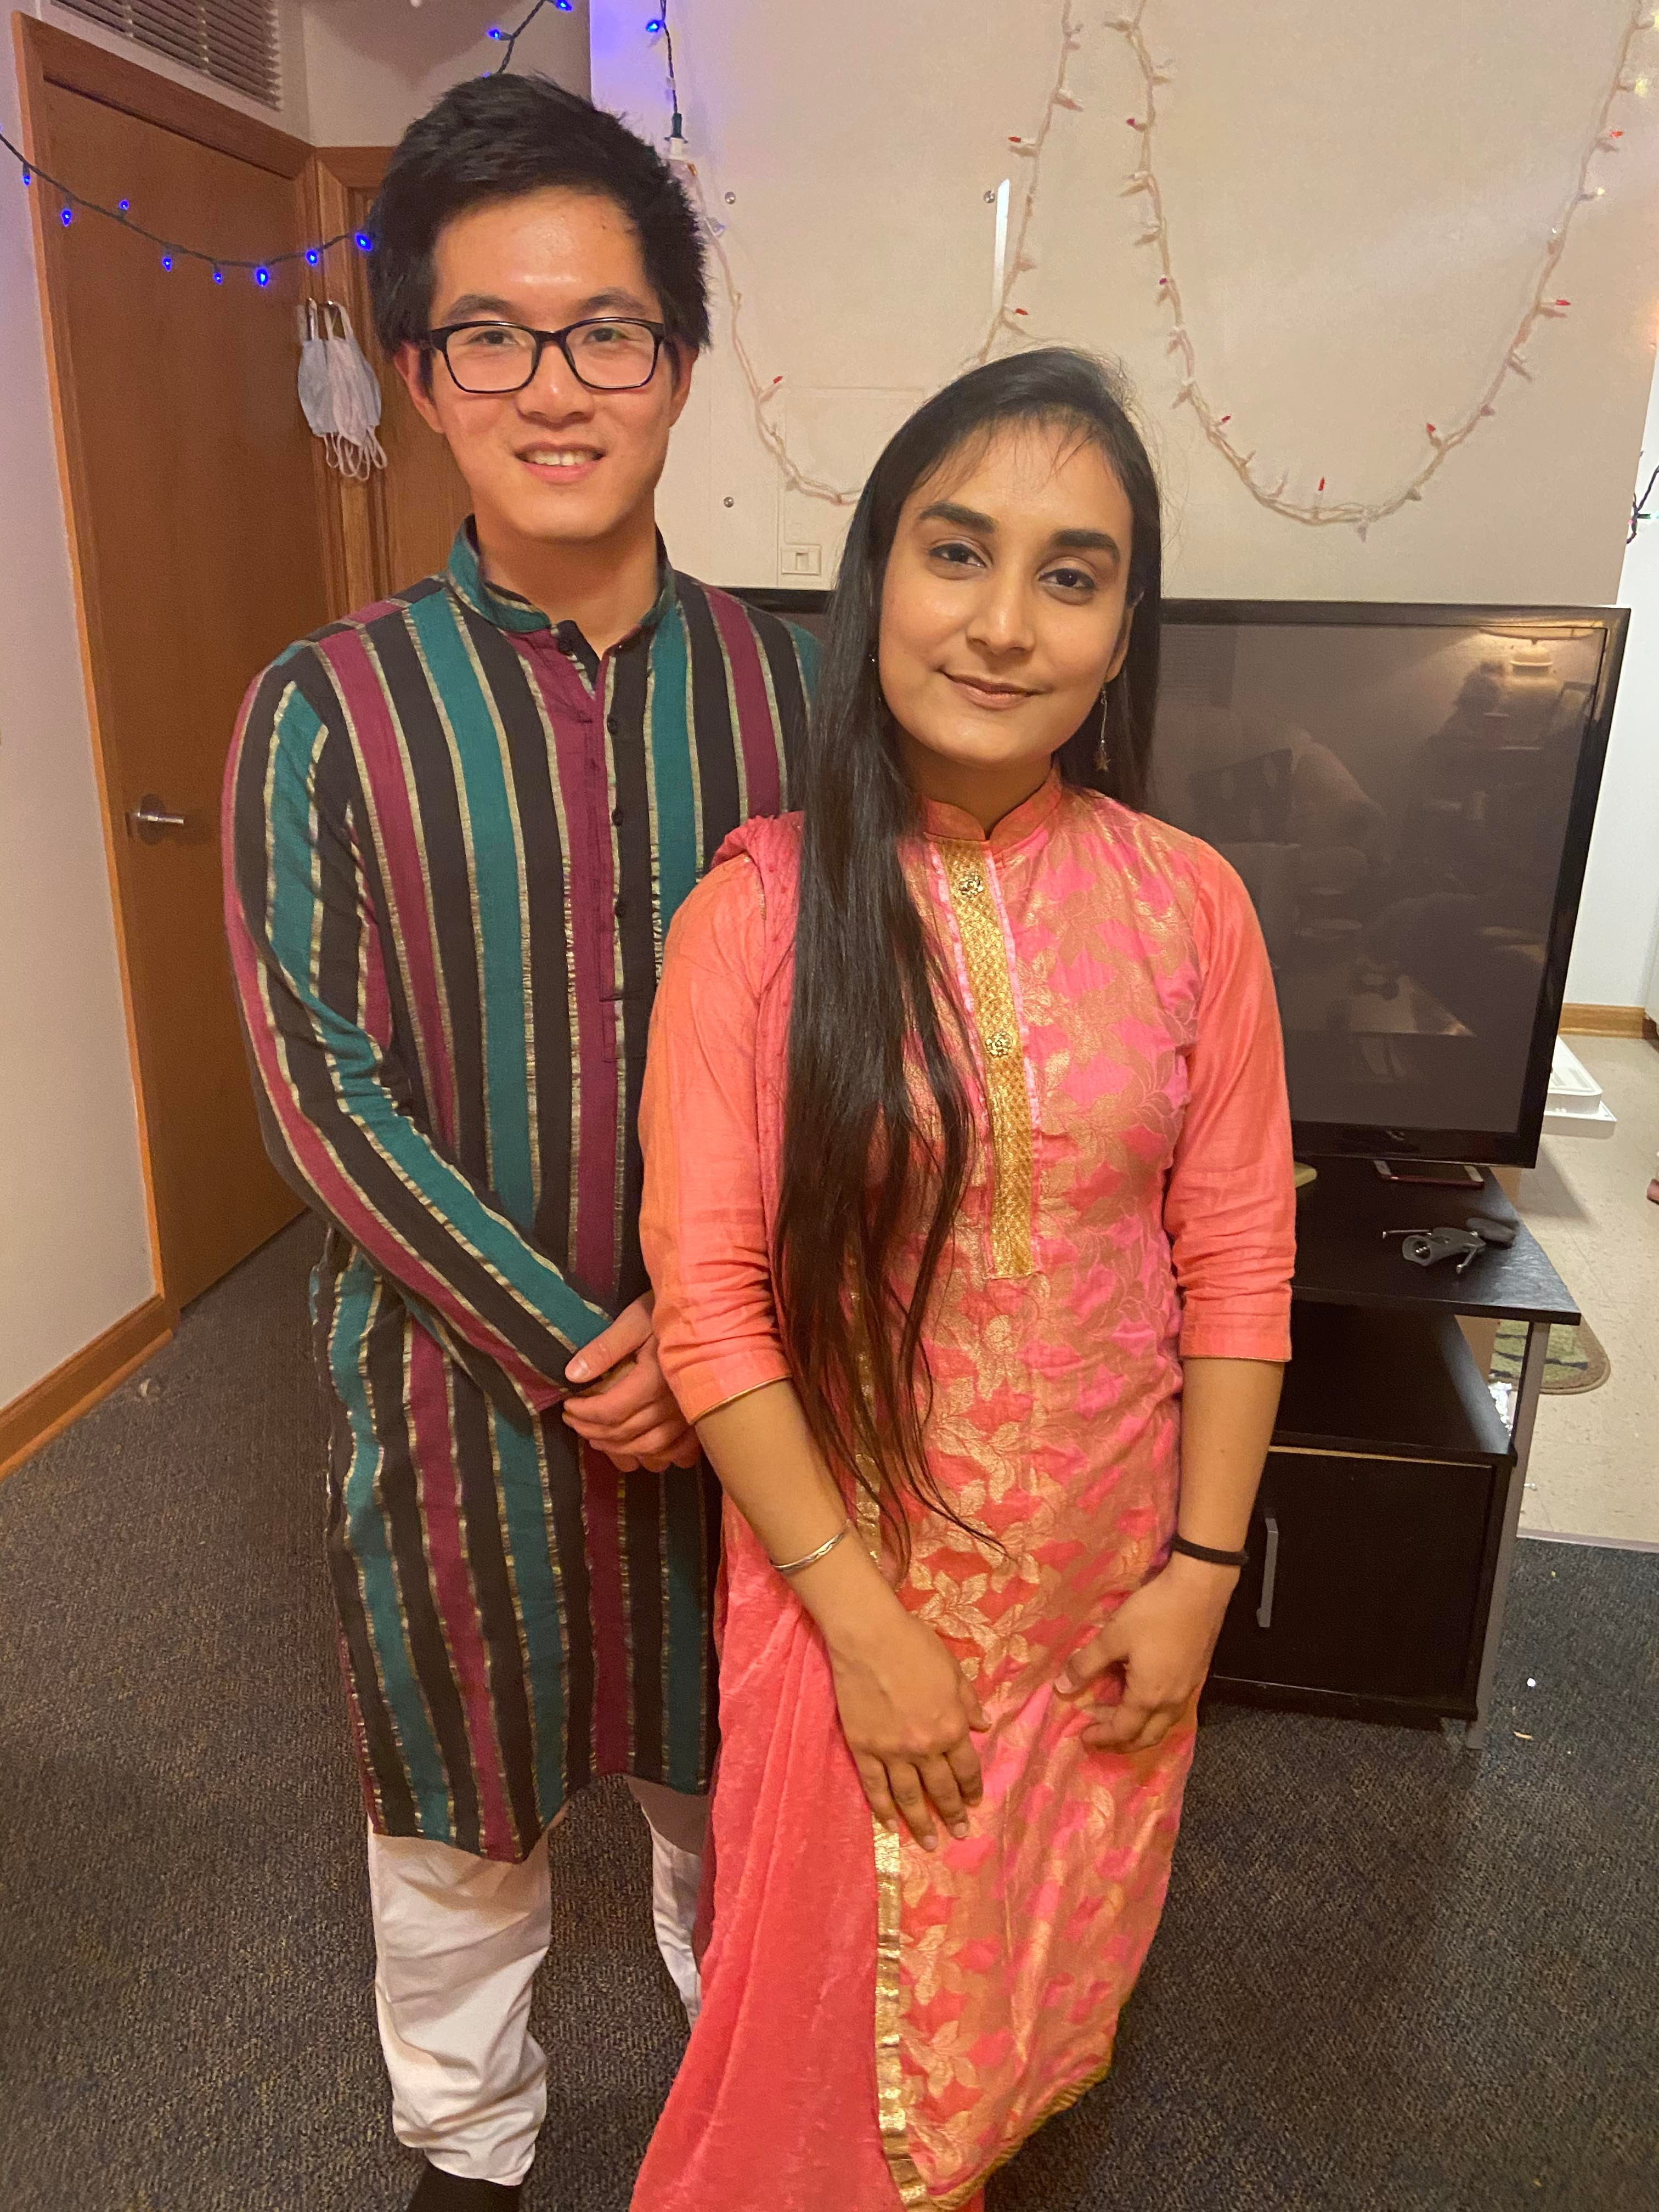
\includegraphics[width=5.20833in,height=\textheight]{mimages/4.1 11-15-2020.jpg}
\caption{November 15, 2020}
\end{figure}

\begin{figure}
\centering
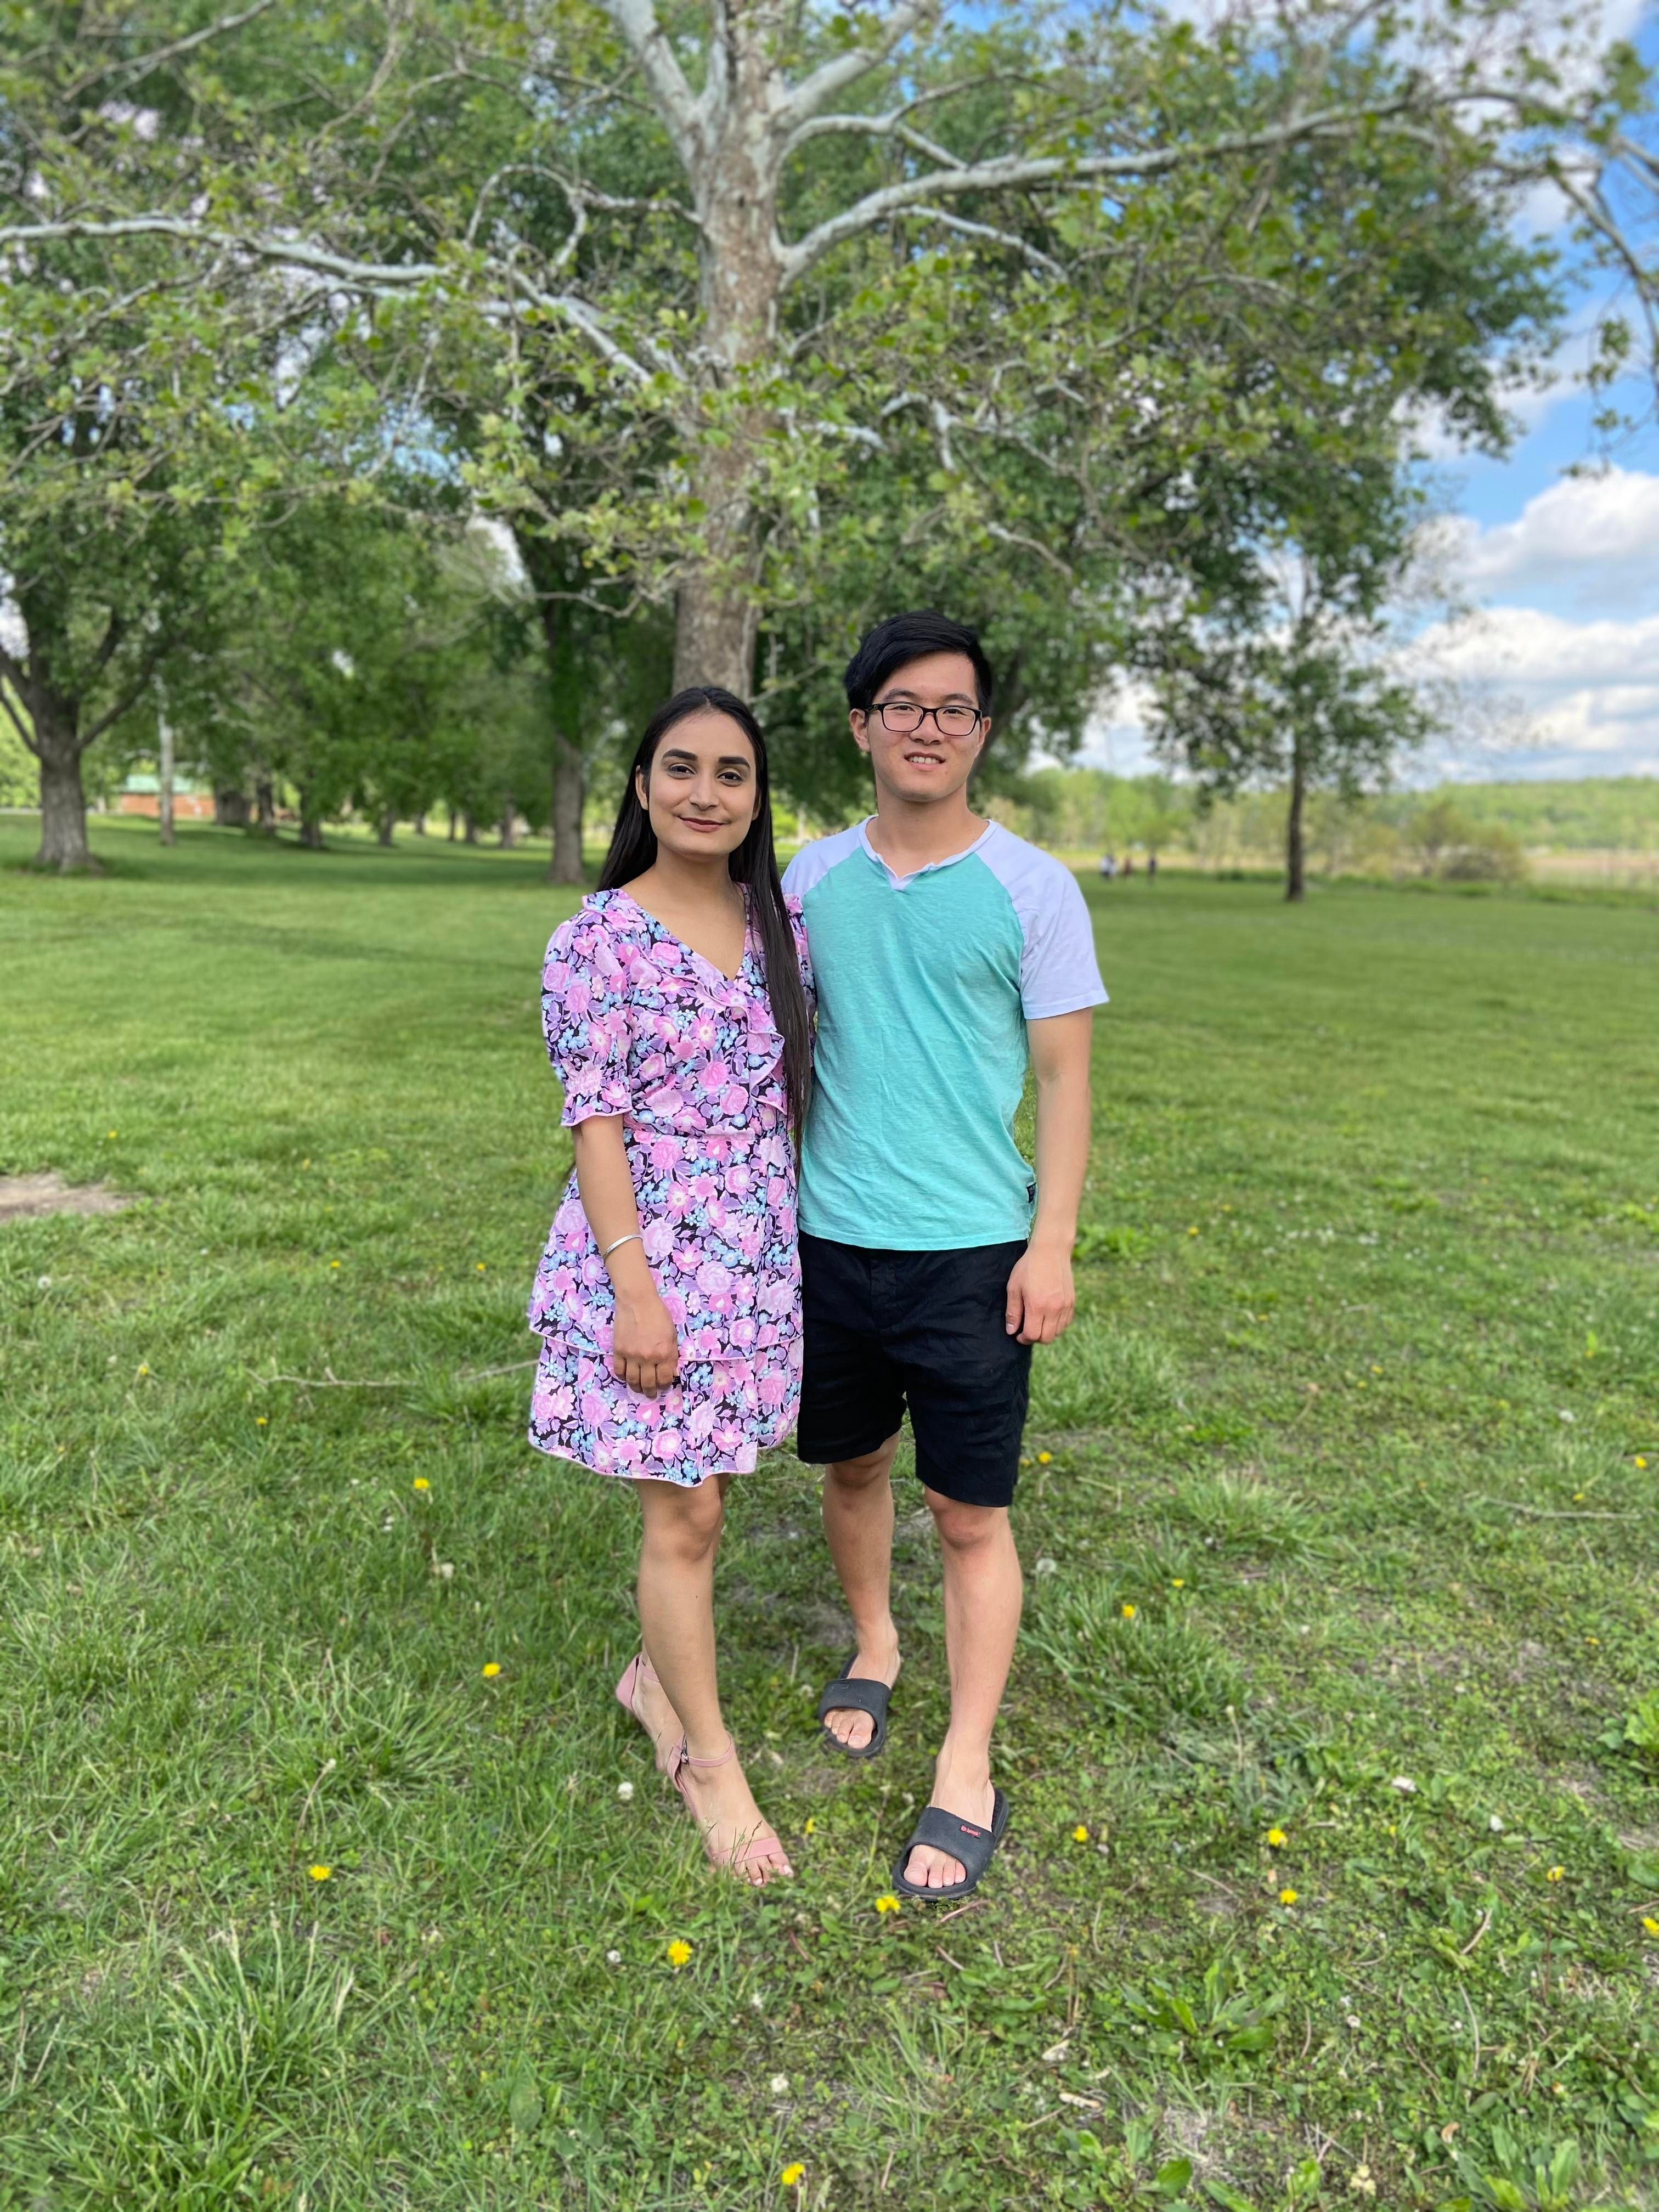
\includegraphics[width=5.20833in,height=\textheight]{mimages/9 5-15-2021.jpg}
\caption{May 15, 2021}
\end{figure}

\hypertarget{a-soft-cough}{%
\chapter{A Soft Cough}\label{a-soft-cough}}

\begin{Shaded}
\begin{Highlighting}[]
\NormalTok{A soft cough,}
\NormalTok{That is good,}
\ControlFlowTok{for}\NormalTok{ clearing a throat.}

\NormalTok{The virtues of voice,}
\NormalTok{Can build our dreams}
\NormalTok{Or corrupt our innocence.  }

\NormalTok{We share out moments,}
\NormalTok{gathering experiences,}
\NormalTok{to link and find ourselves. }

\NormalTok{It can seem exhausting,}
\NormalTok{But a soft cough,}
\NormalTok{Can bring back your breath.}

\NormalTok{But }\ControlFlowTok{for}\NormalTok{ me,}
\NormalTok{a soft cough,}
\NormalTok{can}\StringTok{\textquotesingle{}t bring back my breath.}

\StringTok{For my breath lies in you,}
\StringTok{my future wife, }
\StringTok{you are my life.}
\StringTok{You are my breath   }
\end{Highlighting}
\end{Shaded}

\begin{figure}
\centering
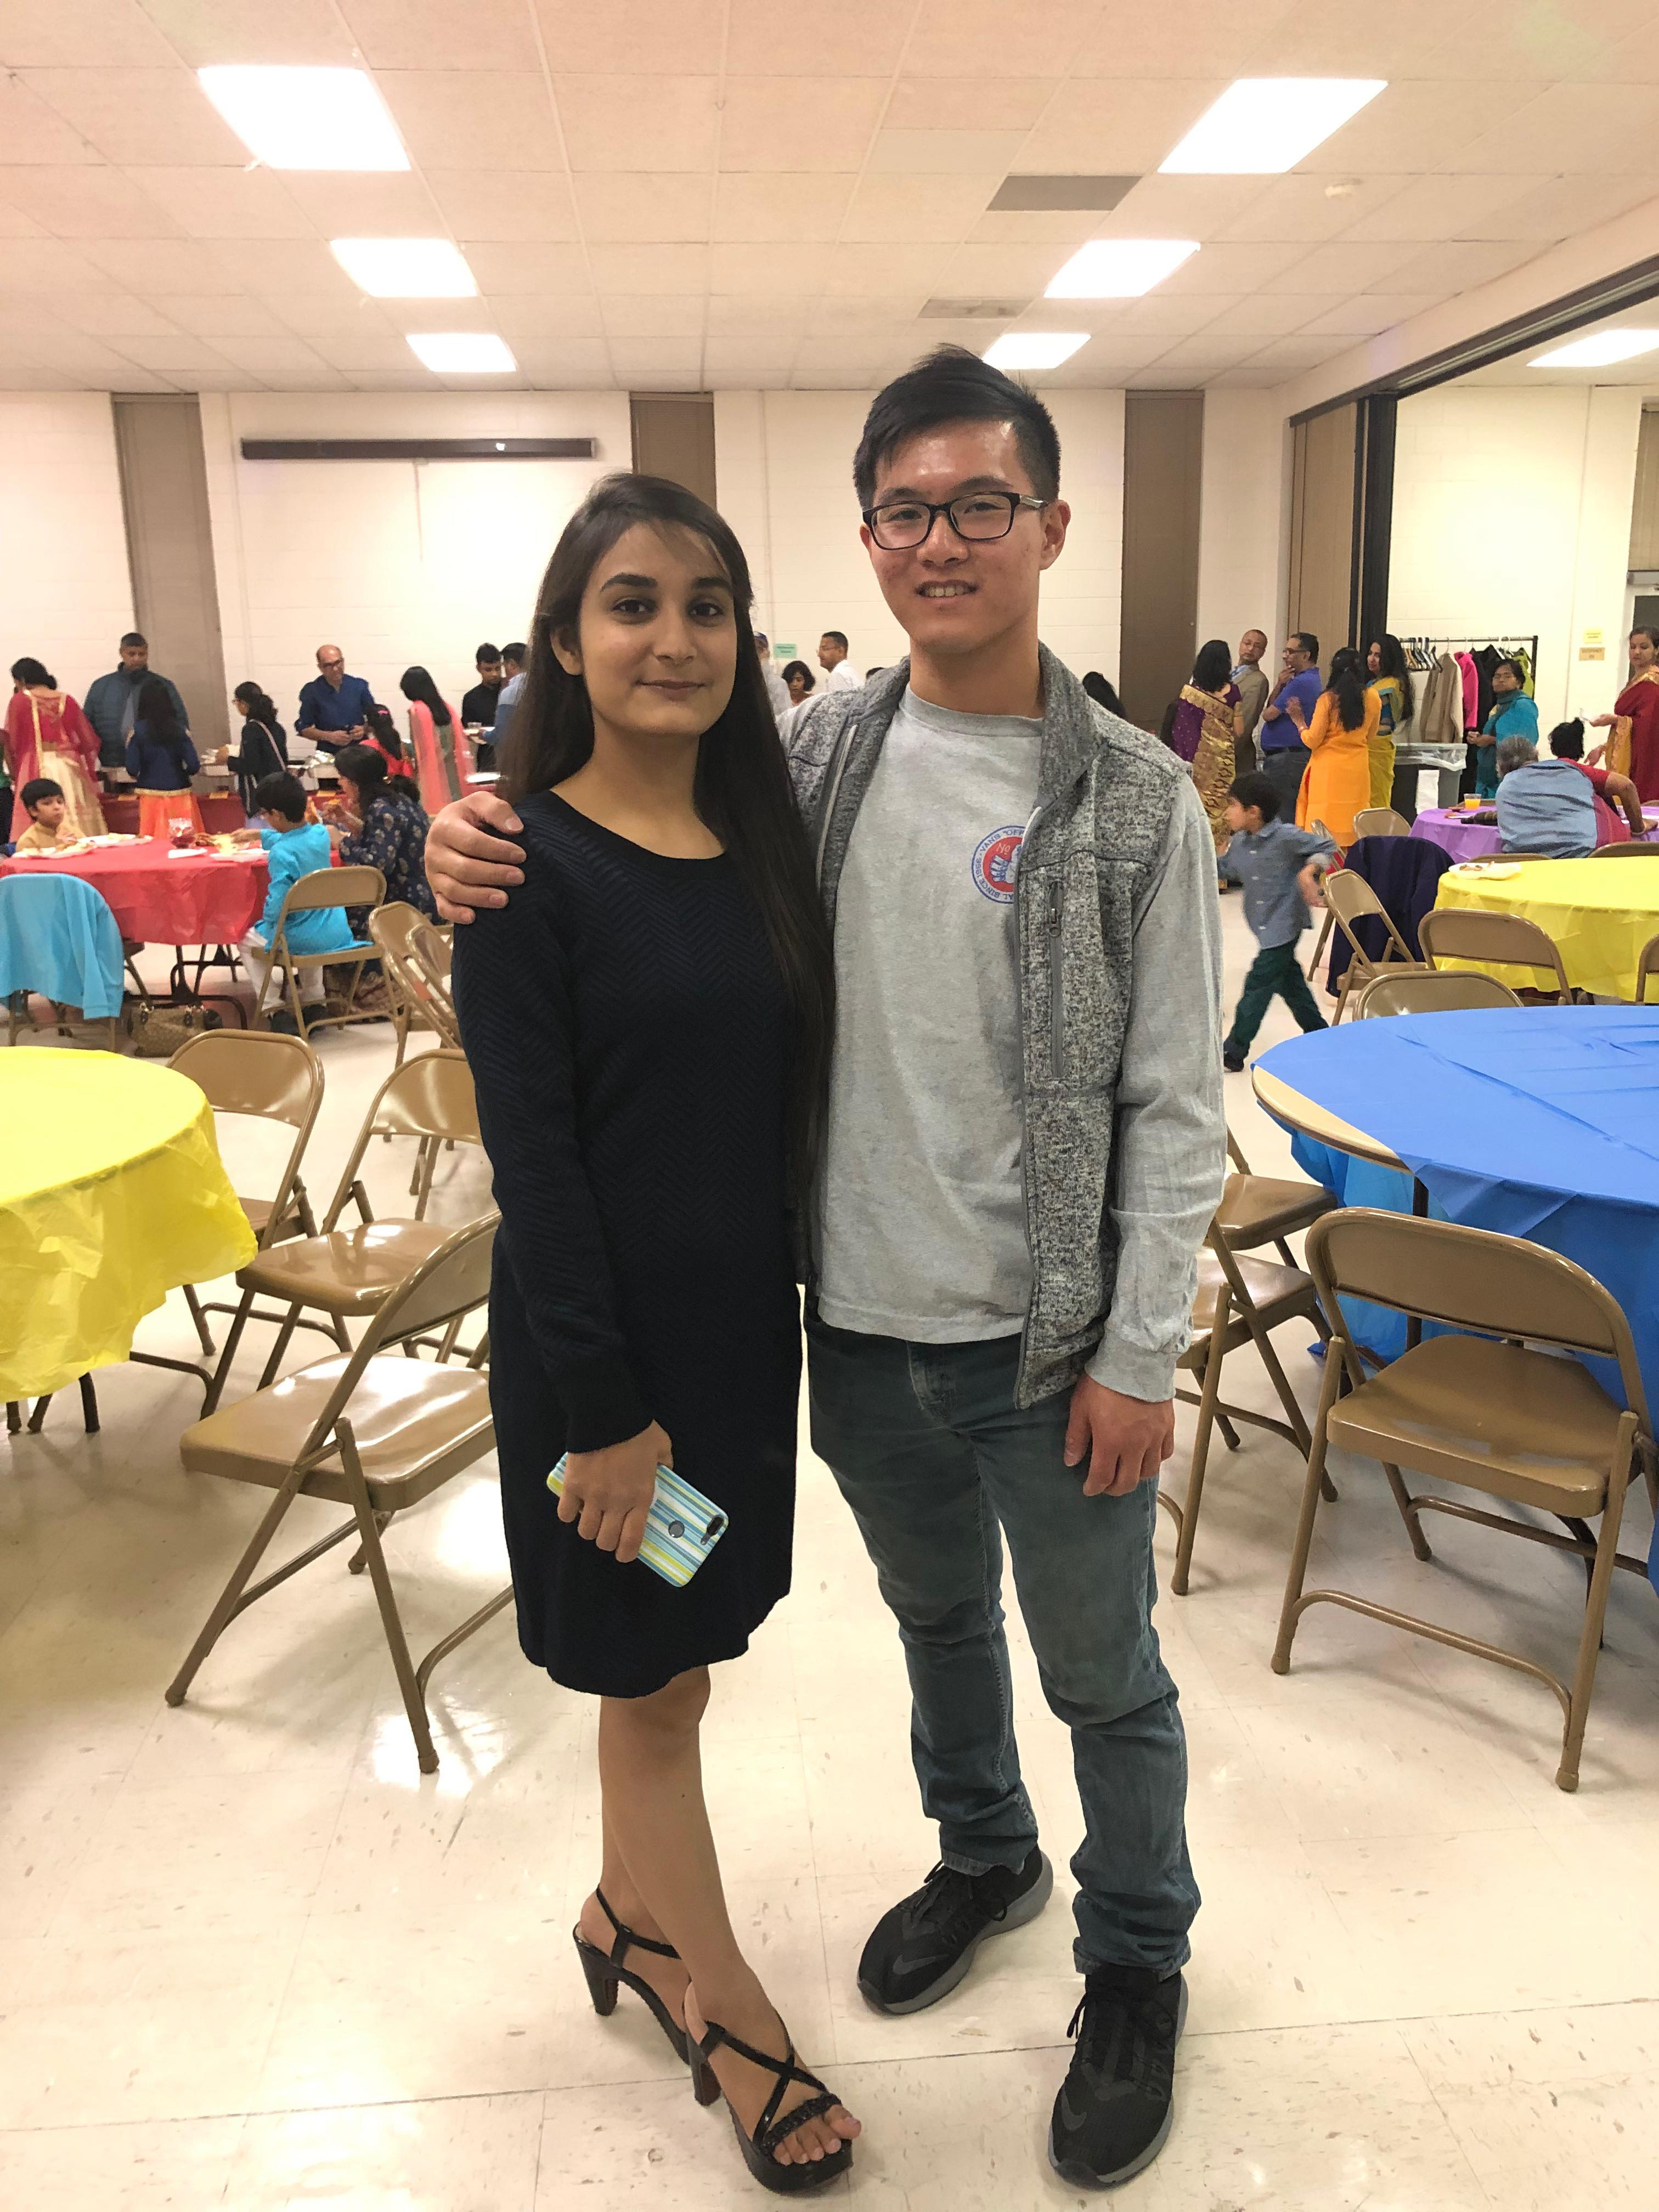
\includegraphics[width=5.20833in,height=\textheight]{mimages/0 8-27-2019.jpg}
\caption{October 27, 2019}
\end{figure}

\begin{figure}
\centering
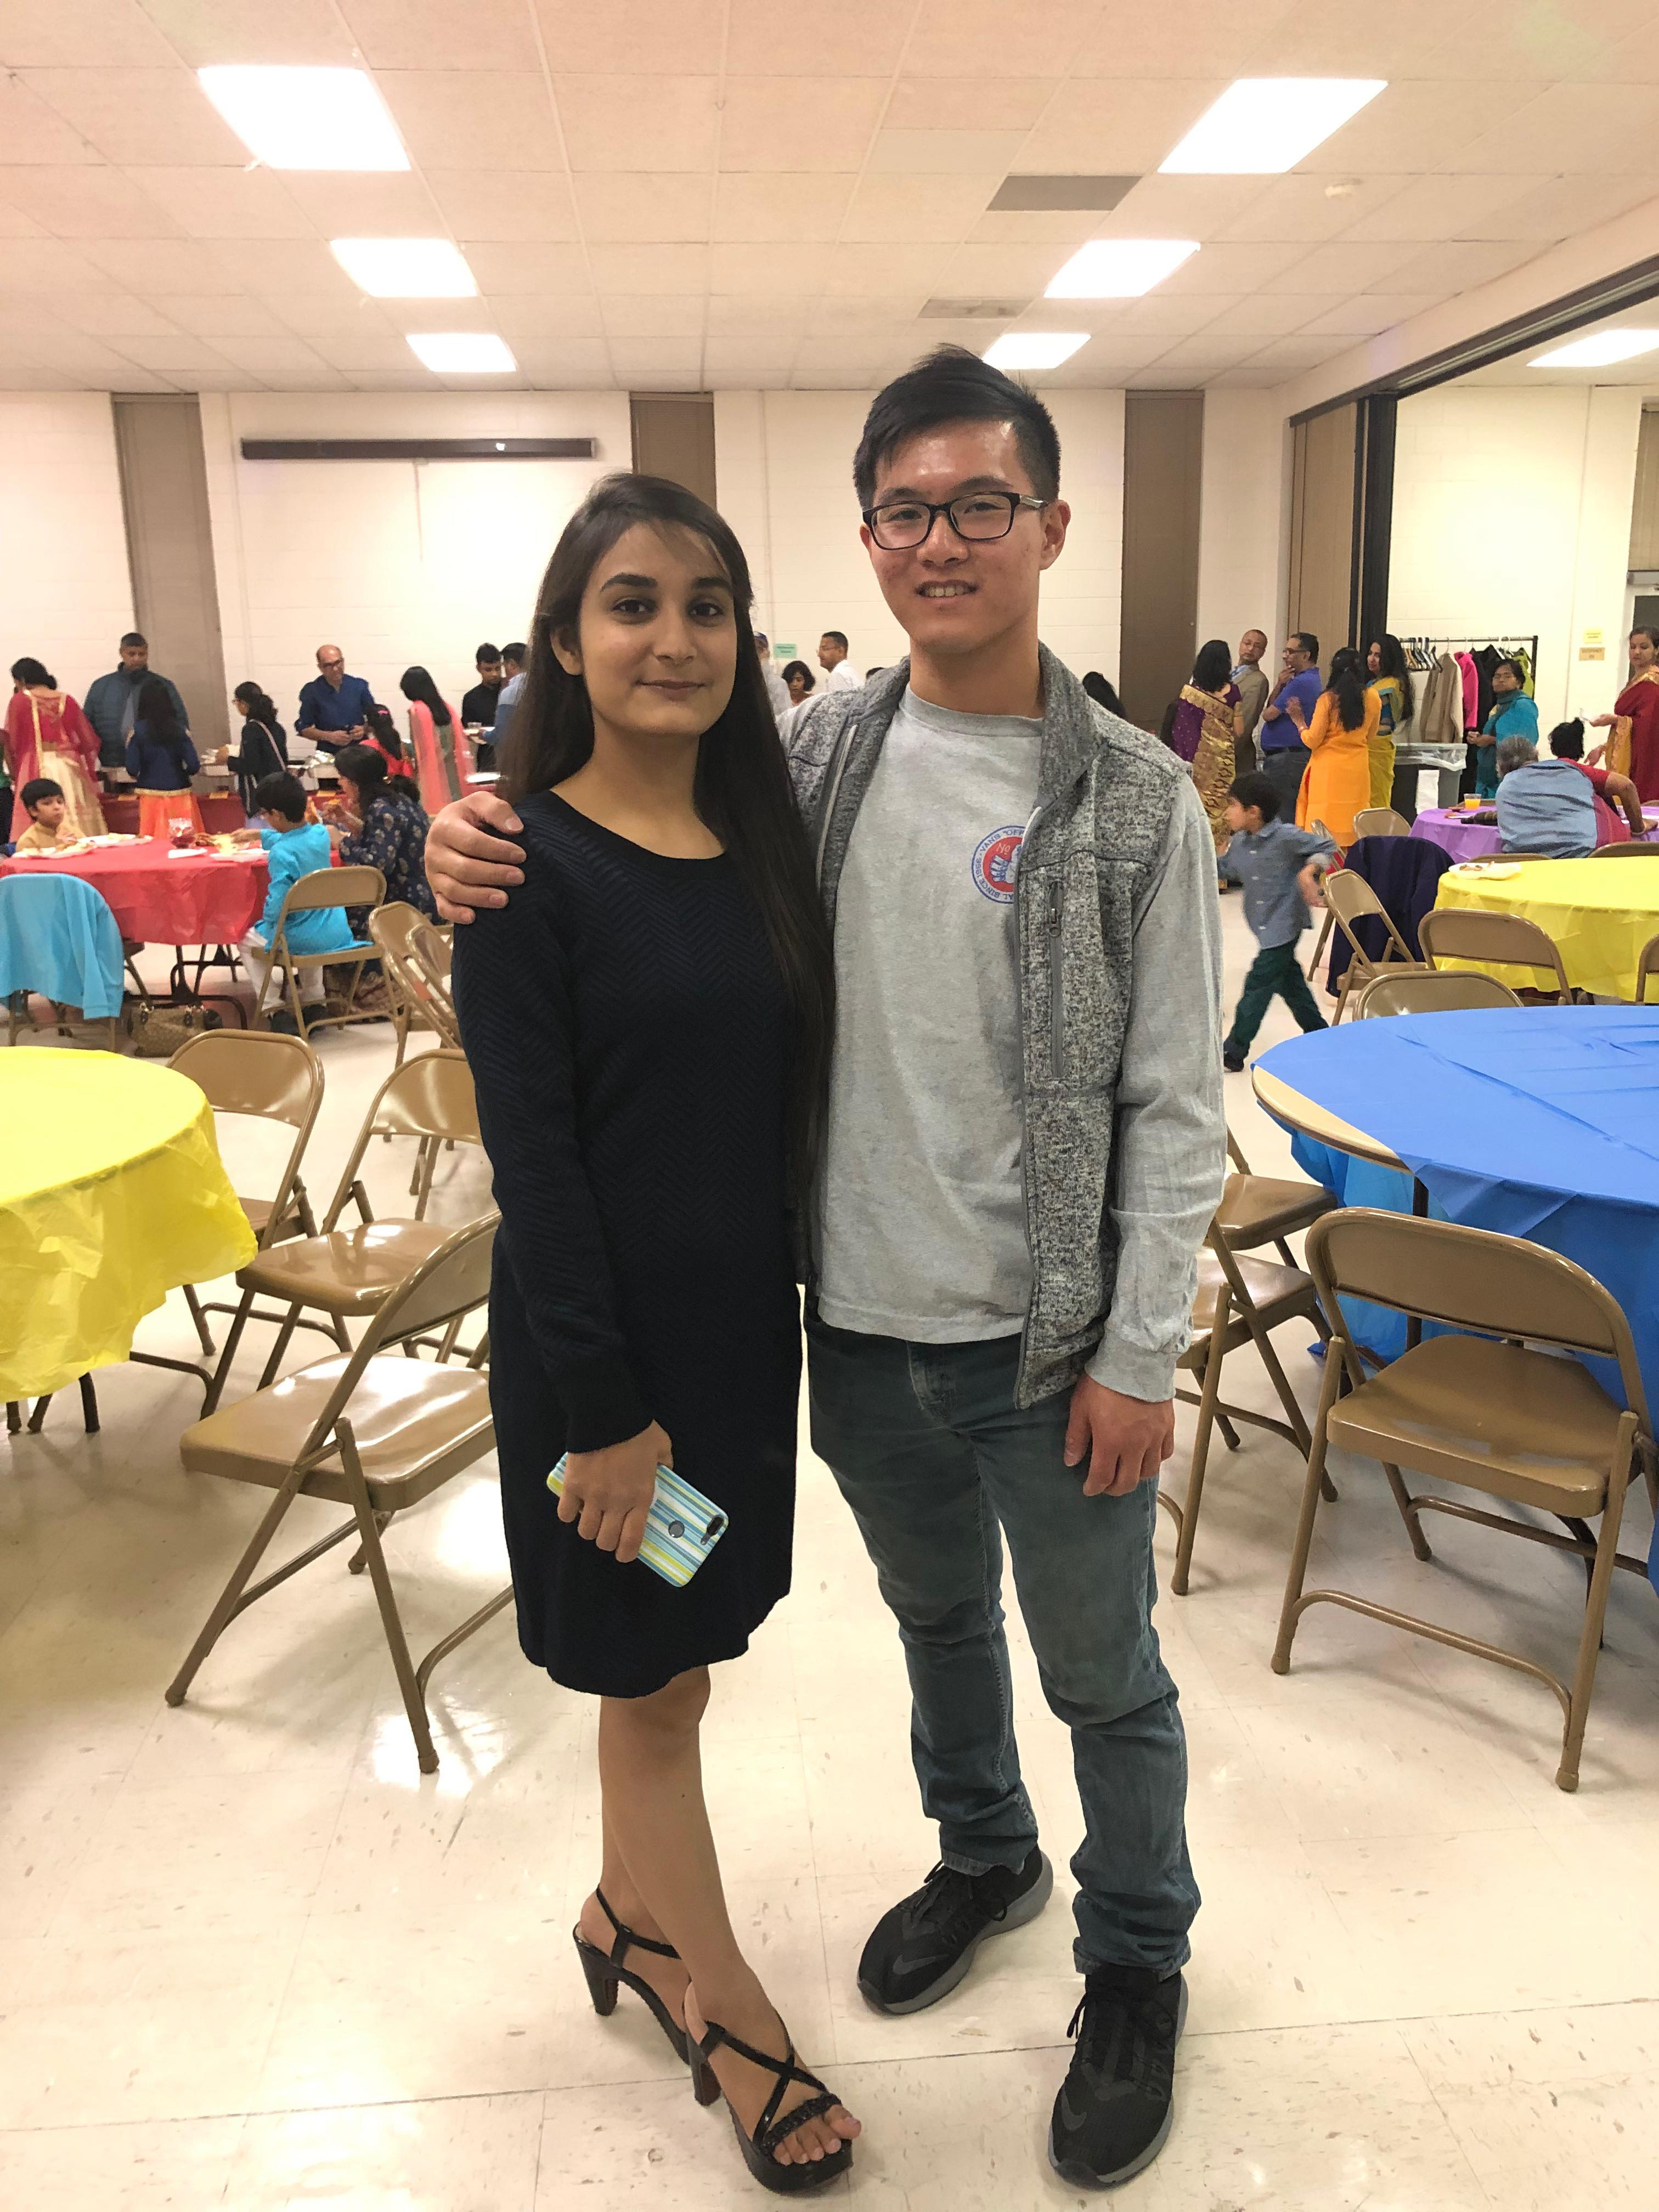
\includegraphics[width=5.20833in,height=\textheight]{mimages/0 8-27-2019.jpg}
\caption{October 27, 2019}
\end{figure}

\begin{figure}
\centering
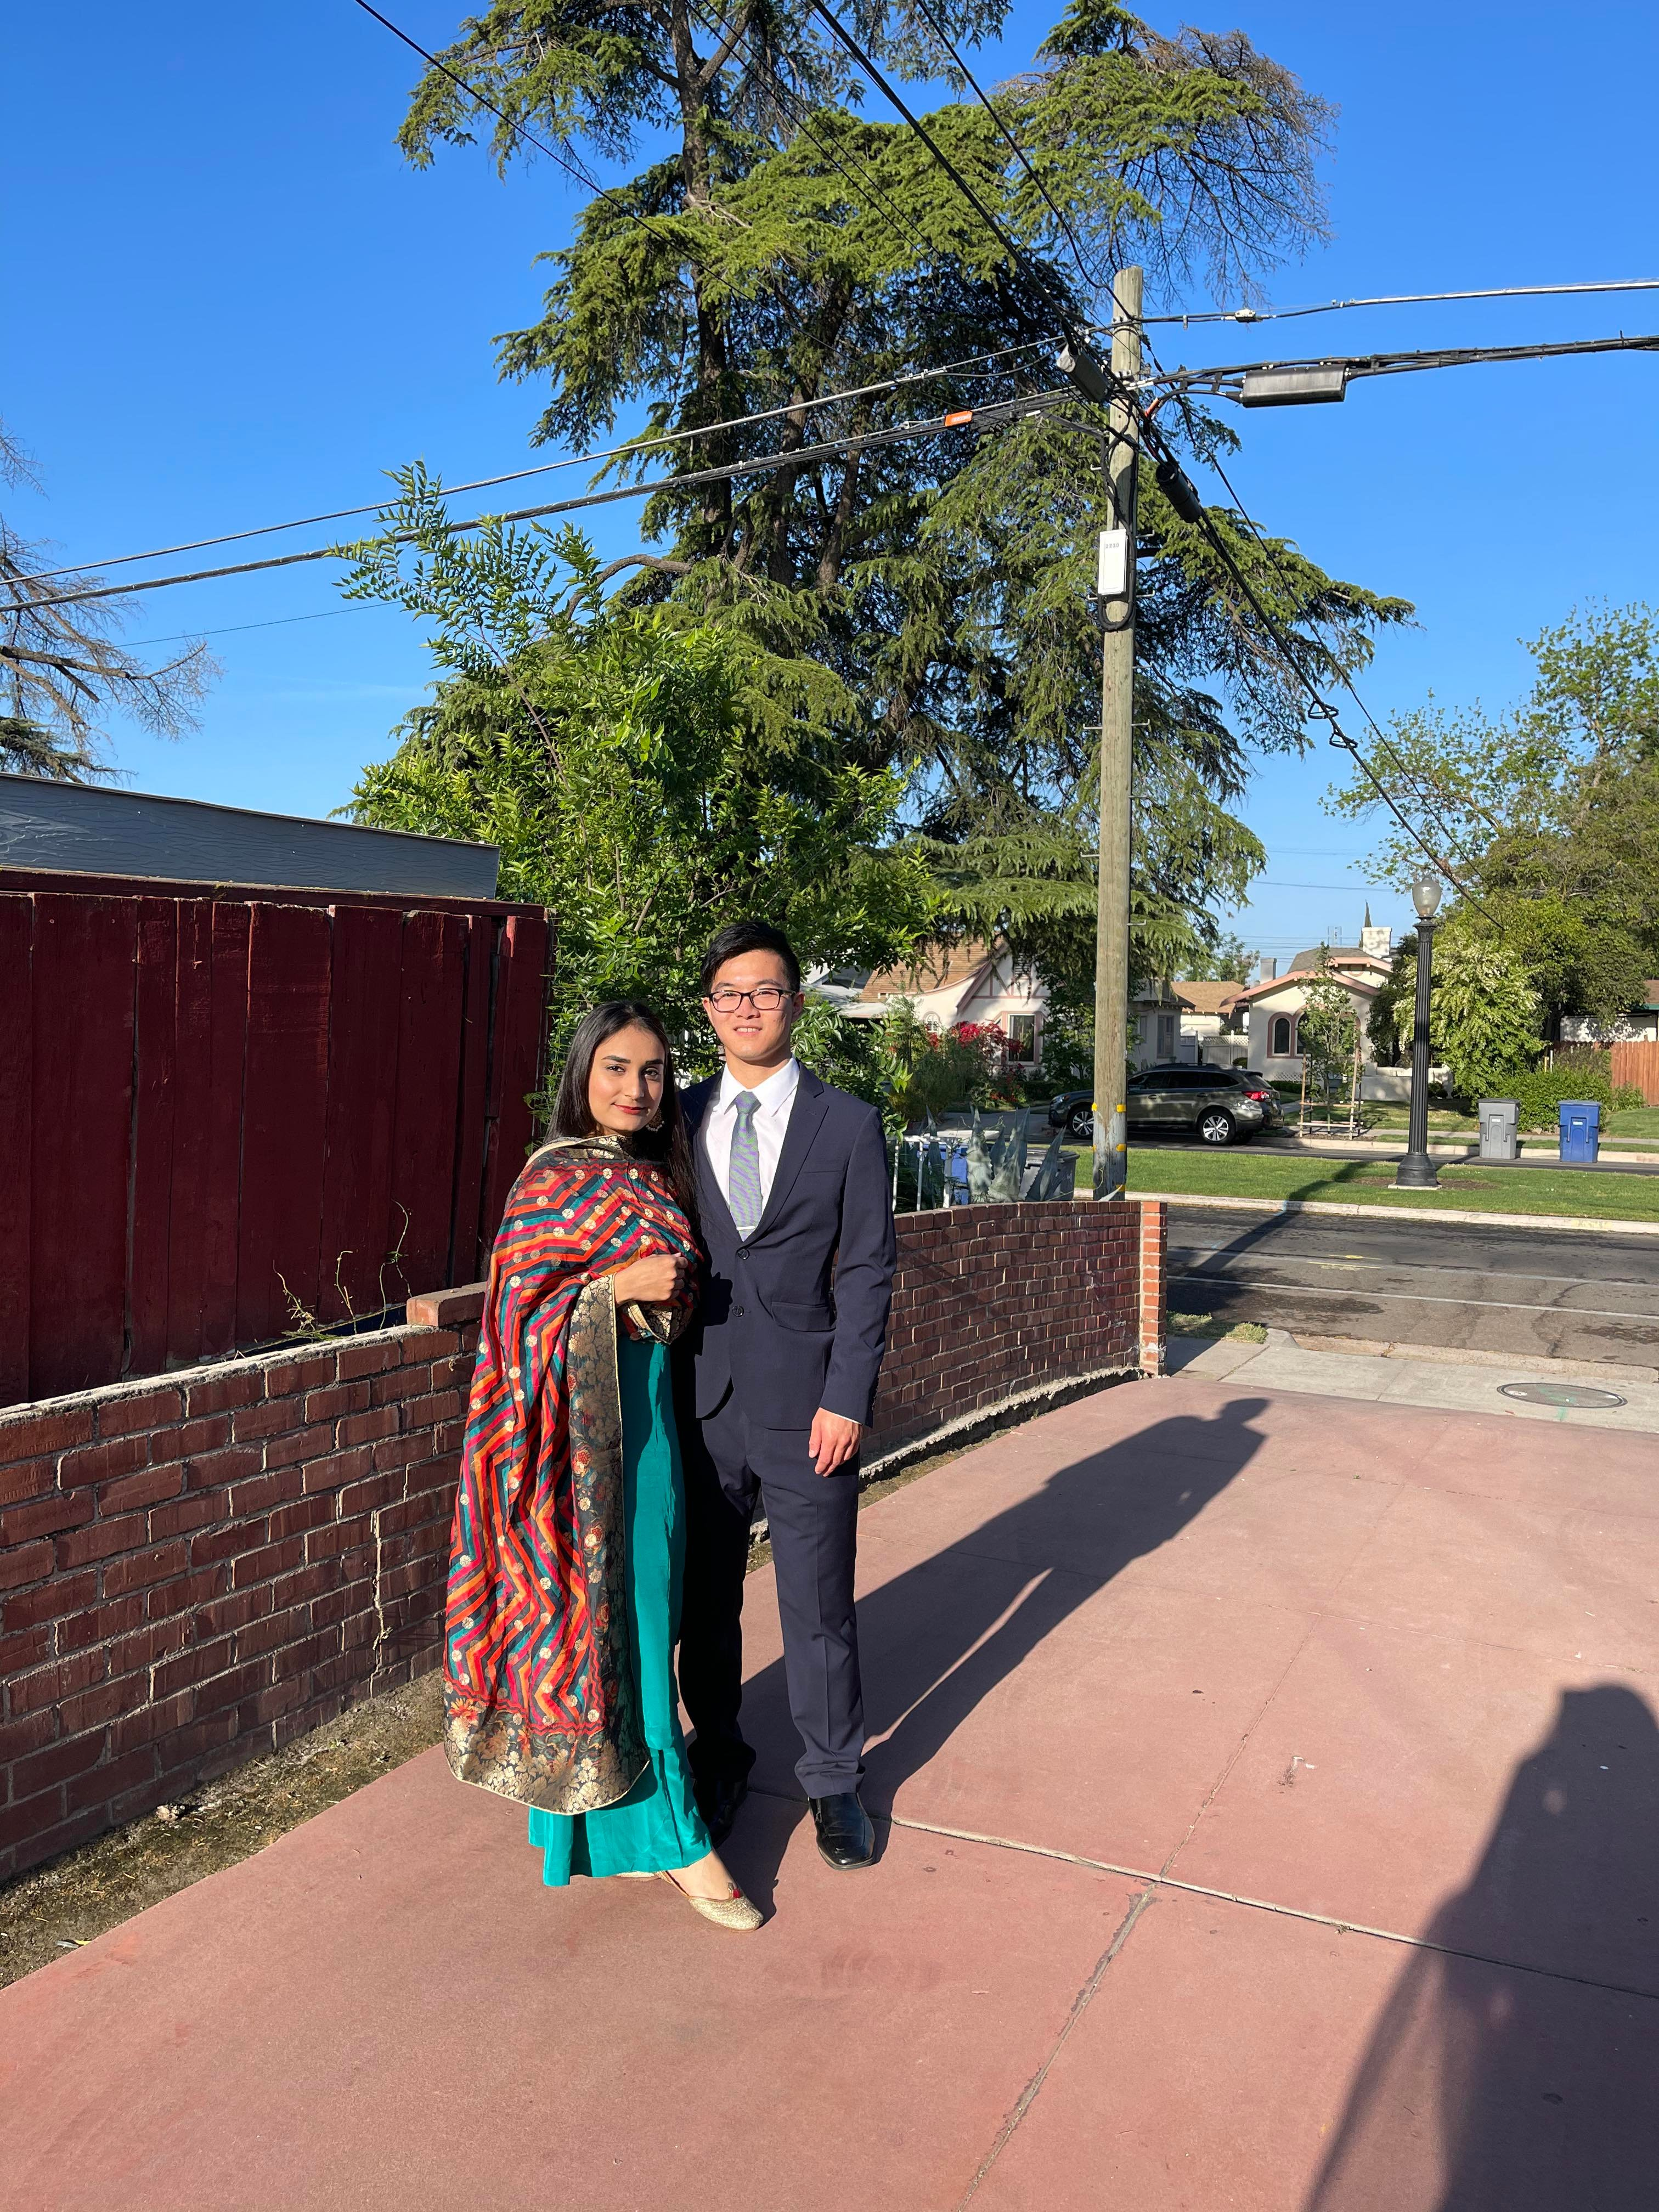
\includegraphics[width=5.20833in,height=\textheight]{mimages/8.3 4-23-2021.jpg}
\caption{April 23, 2021}
\end{figure}

\begin{figure}
\centering
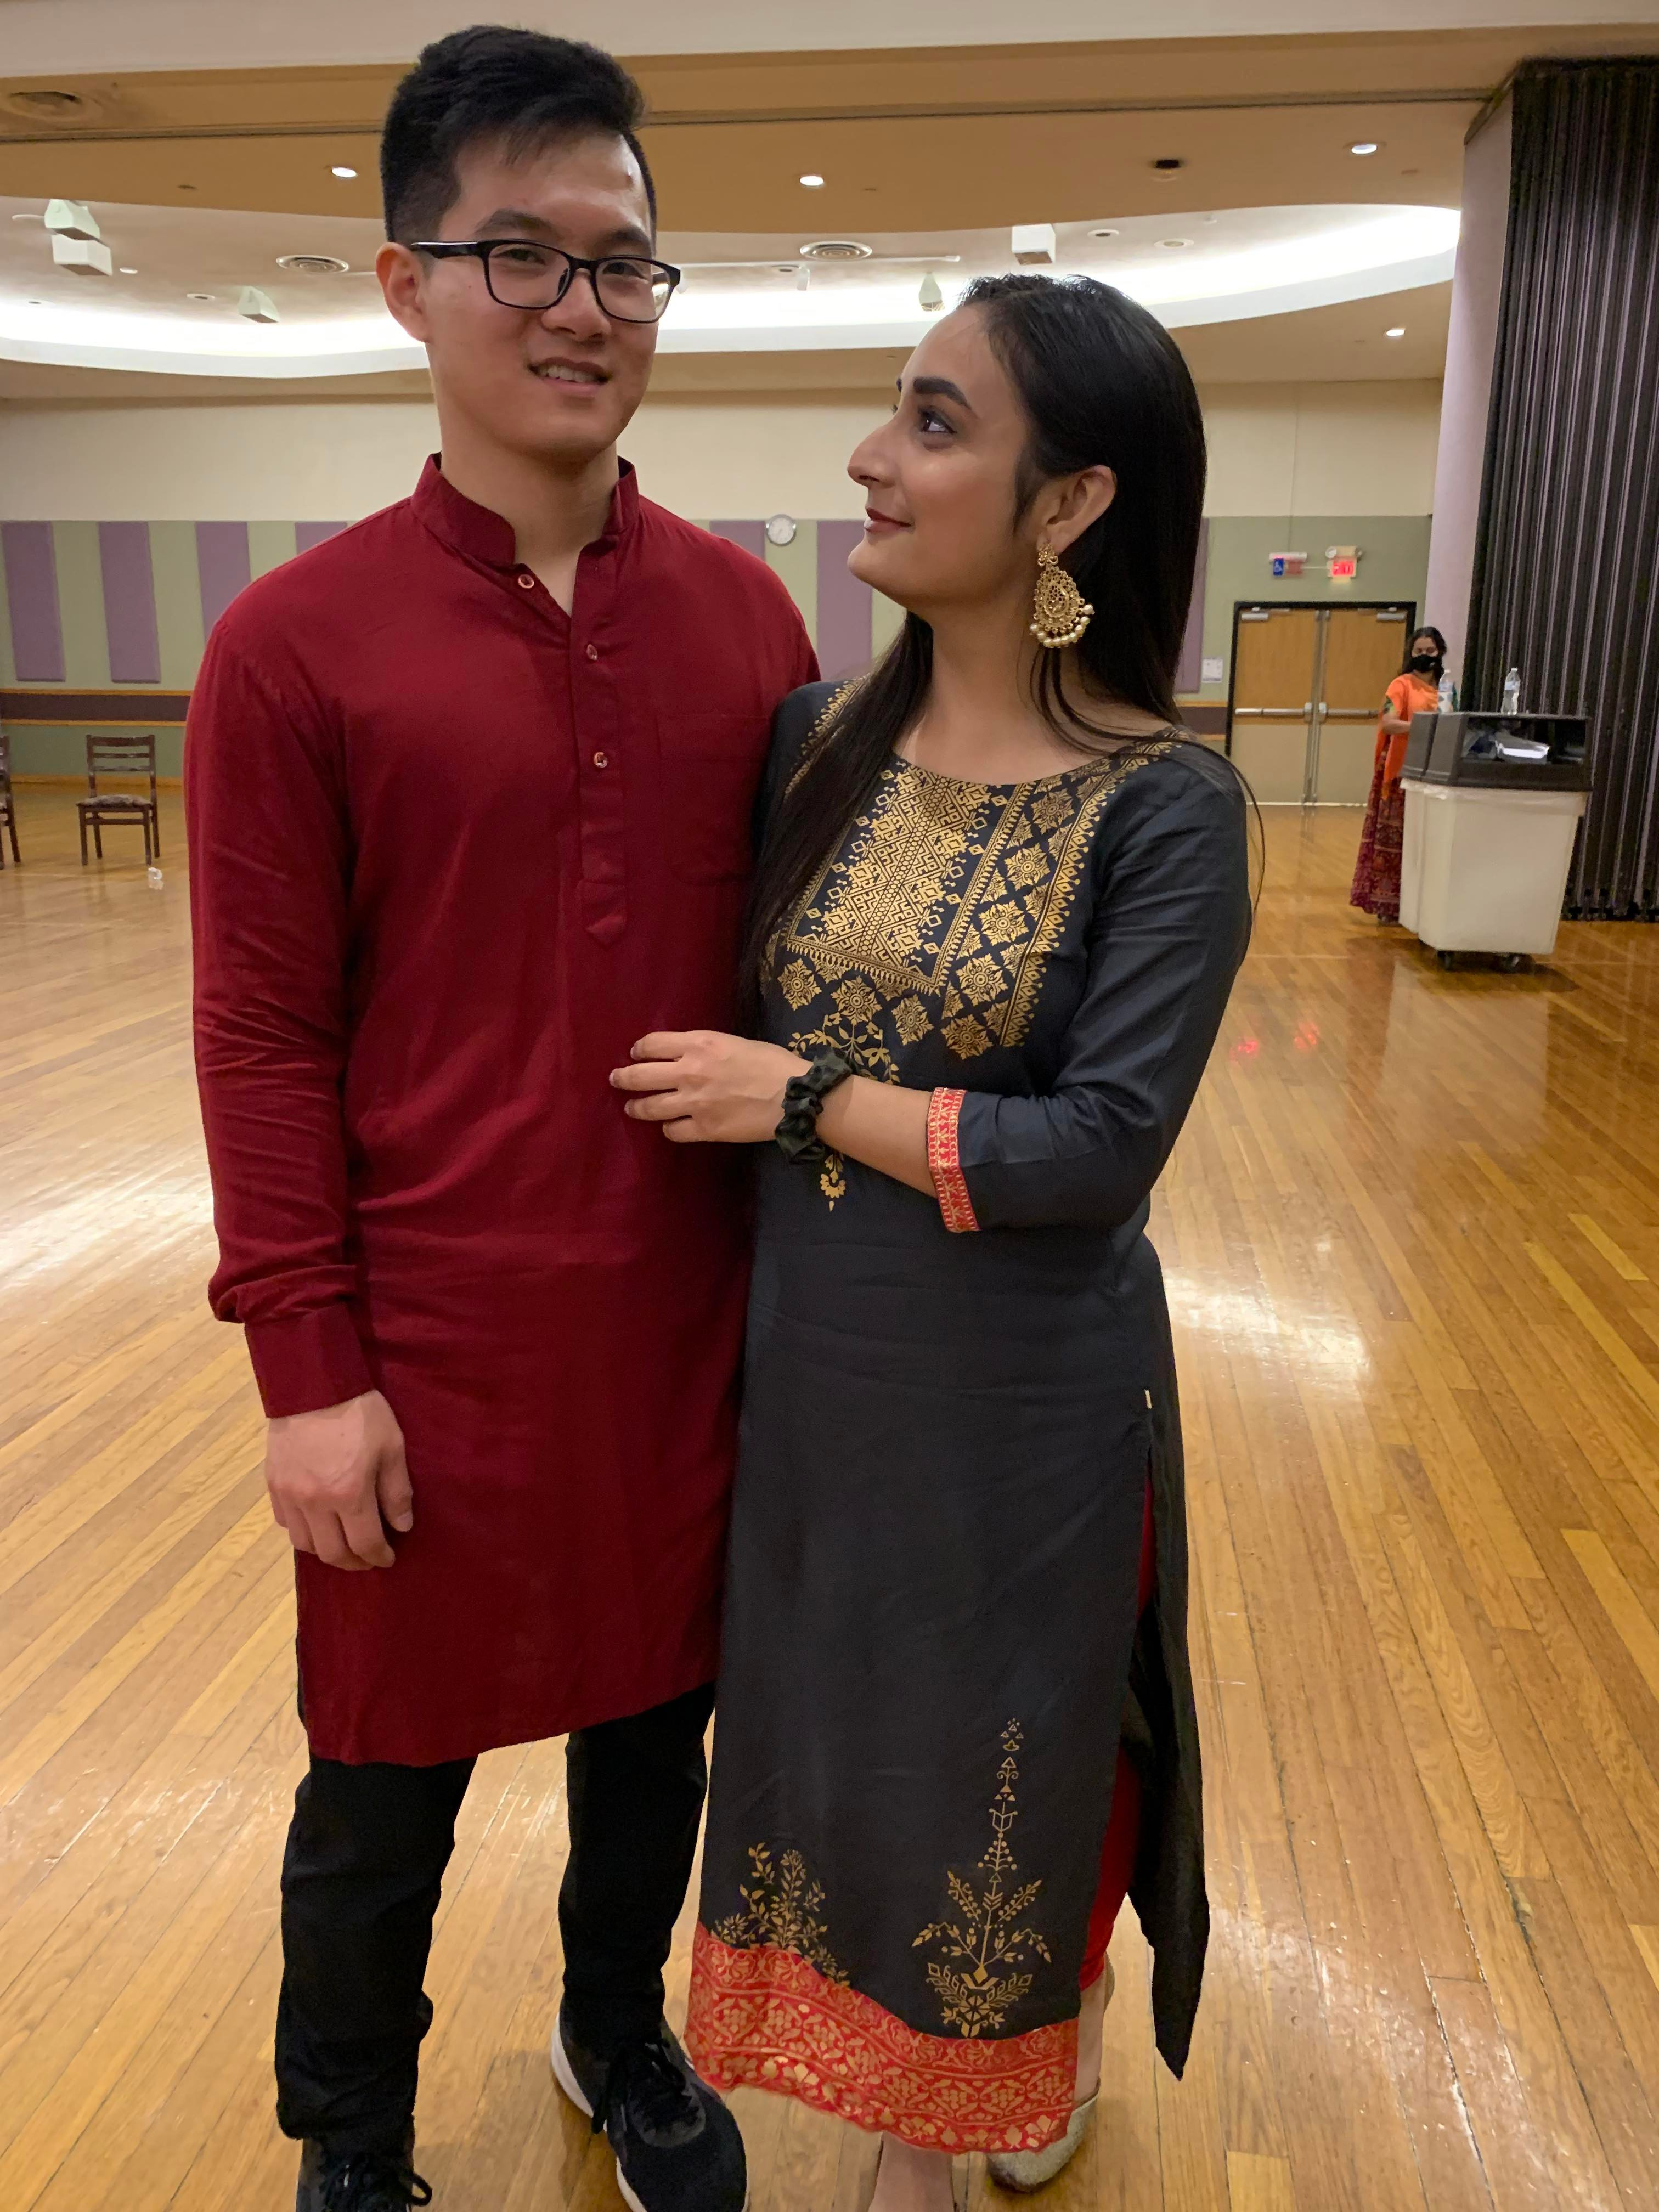
\includegraphics[width=5.20833in,height=\textheight]{mimages/13.3 10-9-2021.jpg}
\caption{October 9, 2021}
\end{figure}

I can only see the world as it should be.

I can not see into people's hearts.

But I know in my heart, I see, you, Manjot Kaur Rekhi.

\begin{figure}
\centering
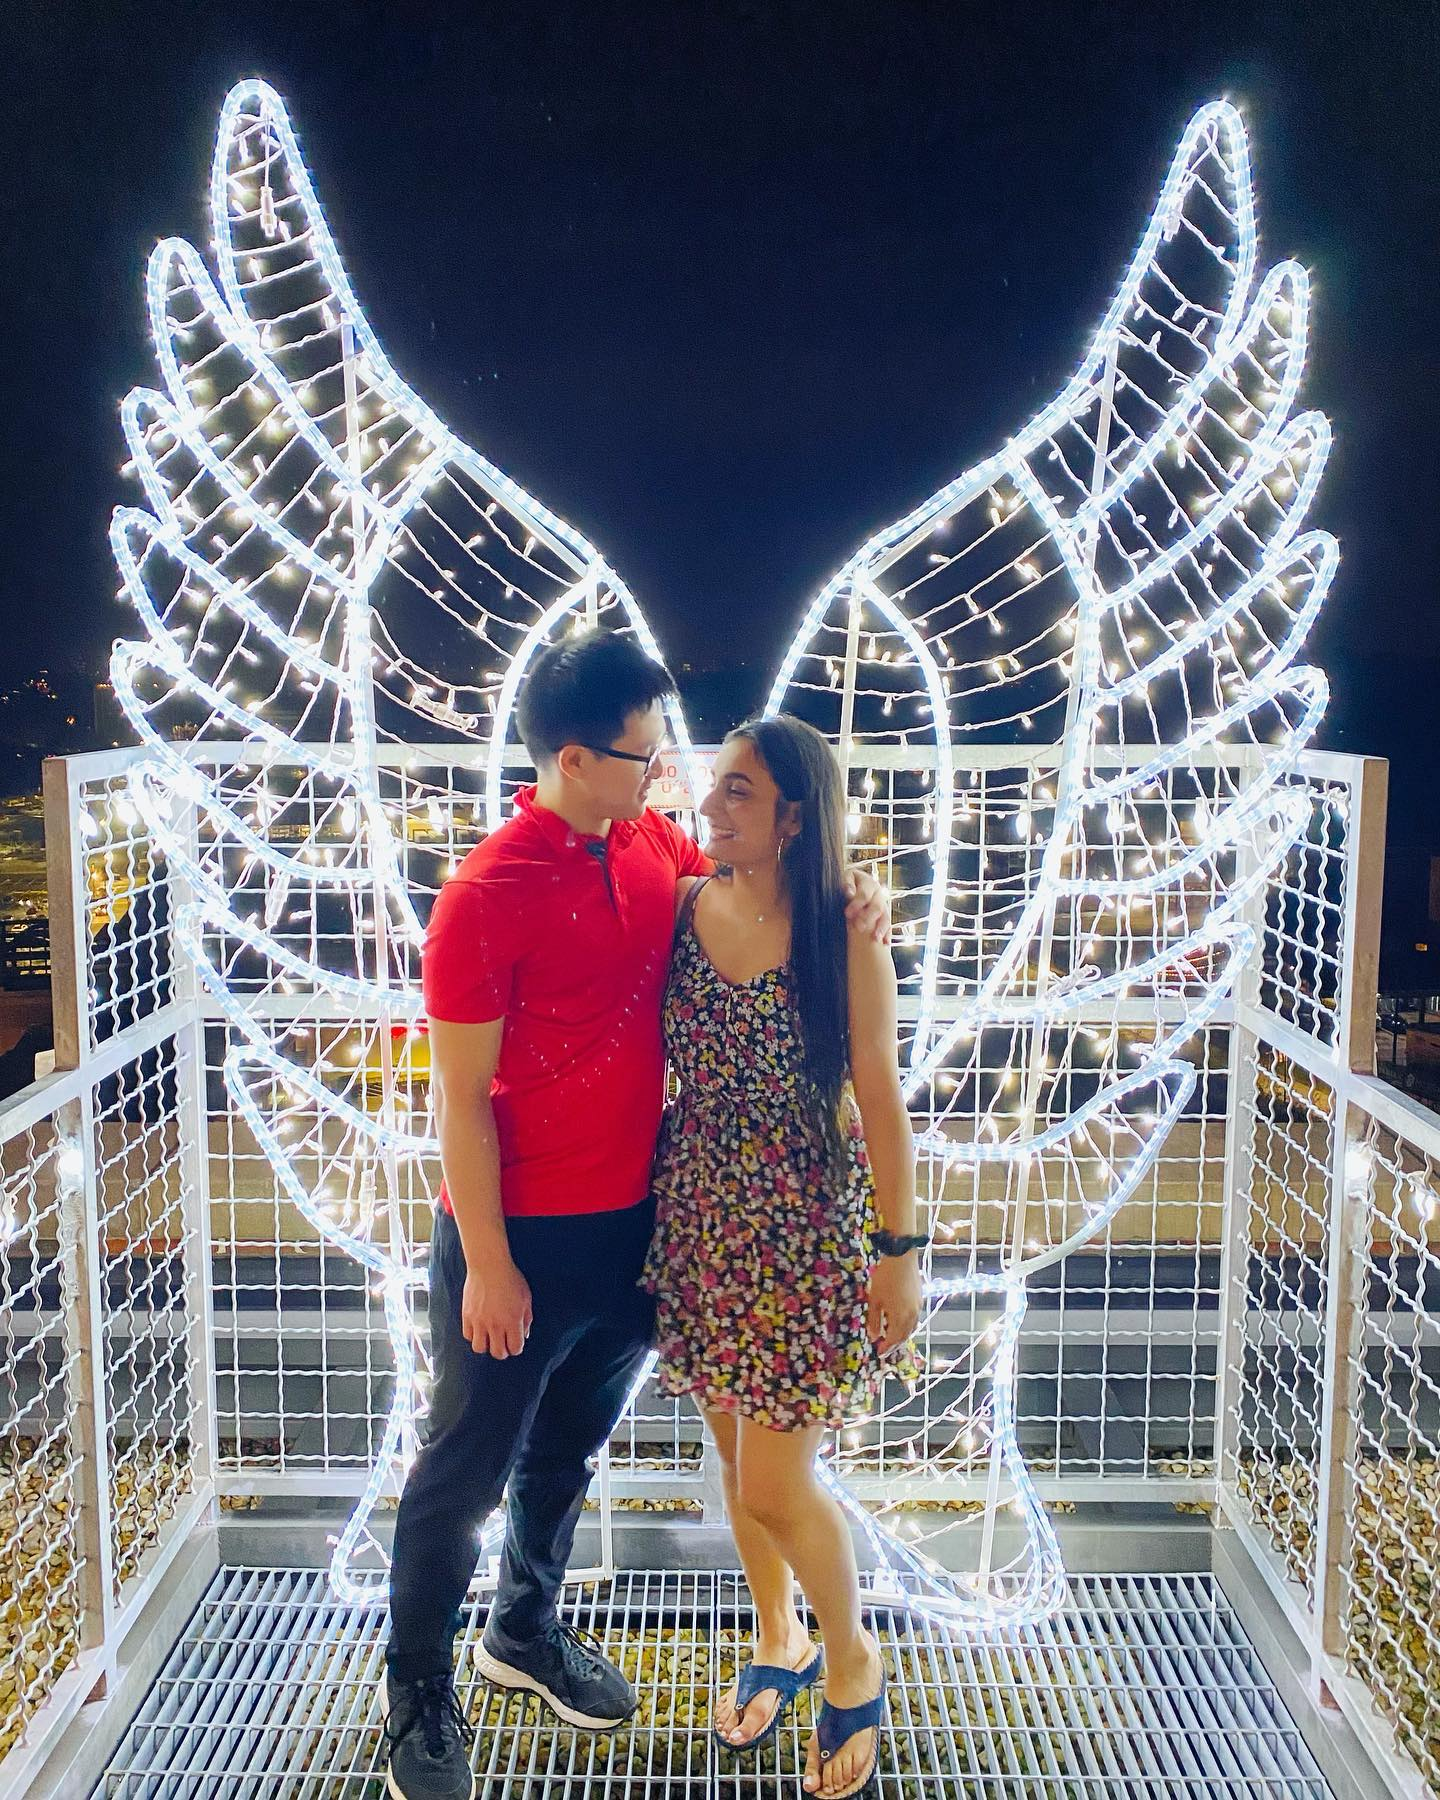
\includegraphics[width=5.20833in,height=\textheight]{mimages/15.1 12-31-2021.jpg}
\caption{December 31, 2021}
\end{figure}

\texttt{**Feel\ free\ to\ skip\ this\ part**}

\hypertarget{set-up}{%
\section{Set up}\label{set-up}}

I used the tutorial from \emph{\url{https://www.youtube.com/watch?v=_ptrgqx2zUs\&ab_channel=AlisonHill}}

\begin{itemize}
\item
  I ran the function \texttt{create\_bs4\_book} in the \texttt{bookdown} package.
\item
  I opened \texttt{\_output.yml} file and changed the repo name to my Github repository URL.
\item
  I changed the color theme- \texttt{primary} by searching colors in \emph{\url{https://coolors.co/}}
\item
  I used \texttt{4A8FE7} - United Nations Blue
\item
  Each \textbf{bookdown} chapter is an .Rmd file, and each .Rmd file can contain one (and only one) chapter. A chapter \emph{must} start with a first-level heading: \texttt{\#\ A\ good\ chapter}, and can contain one (and only one) first-level heading.
\item
  Use second-level and higher headings within chapters like: \texttt{\#\#\ A\ short\ section} or \texttt{\#\#\#\ An\ even\ shorter\ section}.
\item
  The \texttt{index.Rmd} file is required, and is also your first book chapter. It will be the homepage when you render the book.
\end{itemize}

\hypertarget{render-book}{%
\section{Render book}\label{render-book}}

You can render the HTML version of this example book without changing anything:

\begin{enumerate}
\def\labelenumi{\arabic{enumi}.}
\item
  Find the \textbf{Build} pane in the RStudio IDE, and
\item
  Click on \textbf{Build Book}, then select your output format, or select ``All formats'' if you'd like to use multiple formats from the same book source files.
\end{enumerate}

Or build the book from the R console:

\begin{Shaded}
\begin{Highlighting}[]
\NormalTok{bookdown}\SpecialCharTok{::}\FunctionTok{render\_book}\NormalTok{()}
\end{Highlighting}
\end{Shaded}

\hypertarget{preview-book}{%
\section{Preview book}\label{preview-book}}

As you work, you may start a local server to live preview this HTML book. This preview will update as you edit the book when you save individual .Rmd files. You can start the server in a work session by using the RStudio add-in ``Preview book'', or from the R console:

\begin{Shaded}
\begin{Highlighting}[]
\NormalTok{bookdown}\SpecialCharTok{::}\FunctionTok{serve\_book}\NormalTok{()}
\end{Highlighting}
\end{Shaded}

\hypertarget{website-publishing}{%
\section{Website Publishing}\label{website-publishing}}

After adding the poems and pictures, I uploaded the book to Netlify.

\begin{itemize}
\tightlist
\item
  I used the \texttt{\_book} folder for the website
\end{itemize}

Happy reading!

  \bibliography{book.bib,packages.bib}

\end{document}
